%%%%%%%%%%%%%%%%%%%%%%%%%%%%%%%%%%%%%%%%%%%%%%%%%%%
%
%  New template code for TAMU Theses and Dissertations starting Fall 2012.  
%  For more info about this template or the 
%  TAMU LaTeX User's Group, see http://www.howdy.me/.
%
%  Author: Wendy Lynn Turner 
%
%%%%%%%%%%%%%%%%%%%%%%%%%%%%%%%%%%%%%%%%%%%%%%%%%%%

\documentclass[12pt]{report}
\usepackage[letterpaper]{geometry}
\geometry{verbose,tmargin=1.25in,bmargin=1.25in,lmargin=1.4in,rmargin=1.15in}
 \usepackage[doublespacing]{setspace}
 \usepackage{tocloft}
 \usepackage[rm, tiny,center, compact]{titlesec}
 \usepackage{indentfirst}
 \usepackage{etoolbox}
\usepackage{tocvsec2}
 \usepackage[titletoc]{appendix}
 \usepackage{appendix}
 \usepackage{tamuconfig}
\usepackage{rotating}
\usepackage{xspace}
\usepackage{graphicx}
\usepackage{caption, subcaption}
\usepackage{url}
 \usepackage{booktabs}


% Added to fix issues with pdf searching in some versions of LaTeX
%\usepackage[T1]{fontenc}\usepackage{lmodern}
%%%%%%%%%%%%%%%%%%%%%%%%%%%%%

% Hyperref setup below.  You should be able to get away with using uncommenting just the first line.
%\usepackage[hidelinks]{hyperref}

% if \usepackage[hidelinks]{hyperref} doesn't work try this.
% \usepackage{hyperref}  % Hidelinks is an option that removes link visiability.  TAMU Thesis Offices prefers to not see the links. But often doesn't work.  
% 
% \hypersetup{
%     colorlinks=true,
%     linkcolor=black,
%     citecolor=black,
%     filecolor=black,
%     urlcolor=black,
% }
%%%%%%%  End of hyperref setup.  One of these two options should work, but my motto with hyperref is when in doubt, comment it out!
%%%%%%%%%  This hopefully fixes the problem with vertical spacing of section headings at the top of the page..  Commented out in 1.0.7
% \preto\section{%
% \ifnum\value{section}>0\addtocontents{toc}{\vskip-6pt}\fi
% }
% \preto\subsection{%
% \ifnum\value{subsection}=0\addtocontents{toc}{\vskip-6pt}\fi
% \ifnum\value{subsection}>0\addtocontents{toc}{\vskip-6pt}\fi
% } 
%%%%%%%%%%%%%%%%%%%%%%%%%%%%%%%%%%%%%%%%%%%%%%%%%%%%%%

\newcommand{\aetherflow}{{\AE}therFlow\xspace}
\newcommand{\aetherflowcap}{{\AE}THERFLOW\xspace}
\newcommand{\crossflow}{CrossFlow\xspace}
\newcommand{\crossflowcap}{CROSSFLOW\xspace}

\hyphenation{of-soft-switch}

\newcommand\blfootnote[1]{%
  \begingroup
  \renewcommand\thefootnote{}\footnote{#1}%
  \addtocounter{footnote}{-1}%
  \endgroup
}

\begin{document}

\renewcommand{\tamumanuscripttitle}{Towards a Principled Wireless Support in SDN}
\renewcommand{\tamupapertype}{Thesis}
\renewcommand{\tamufullname}{Prithviraj Shome}
\renewcommand{\tamudegree}{Master of Science}
\renewcommand{\tamuchairone}{Alex Sprintson}
% Uncomment out the next line if you have co-chairs.  You will also need to edit the titlepage.tex file.
\newcommand{\tamuchairtwo}{Additional Chair Name}
\renewcommand{\tamumemberone}{Paul Gratz}
\newcommand{\tamumembertwo}{Radu Stoleru}
\newcommand{\tamumemberthree}{}
\renewcommand{\tamudepthead}{Miroslav M. Begovic}
\renewcommand{\tamugradmonth}{May}
\renewcommand{\tamugradyear}{2016}
\renewcommand{\tamudepartment}{Computer Engineering}


%%%%%%%%%%%%%%%%%%%%%%%%%%%%%%%%%%%%%%%%%%%%%%%%%%%
%
%  New template code for TAMU Theses and Dissertations starting Fall 2012.  
%  For more info about this template or the 
%  TAMU LaTeX User's Group, see http://www.howdy.me/.
%
%  Author: Wendy Lynn Turner 
%	 Version 1.0 
%  Last updated 8/5/2012
%
%%%%%%%%%%%%%%%%%%%%%%%%%%%%%%%%%%%%%%%%%%%%%%%%%%%

%%%%%%%%%%%%%%%%%%%%%%%%%%%%%% 
%% TITLE PAGE
%% The values get updated automatically.  Please do not make changes to this file other than adding/deleting committee members where necessary.
%%%%%%%%%%%%%%%%%%%%%%%%%%%%%%

\providecommand{\tabularnewline}{\\}



\begin{titlepage}
\begin{center}
\MakeUppercase{\tamumanuscripttitle}
\vspace{4em}

A \tamupapertype

by

\MakeUppercase{\tamufullname}

\vspace{4em}

\begin{singlespace}

Submitted to the Office of Graduate and Professional Studies of \\
Texas A\&M University \\

in partial fulfillment of the requirements for the degree of \\
\end{singlespace}

\MakeUppercase{\tamudegree}
\par\end{center}
\vspace{2em}
\begin{singlespace}
\begin{tabular}{ll}
 & \tabularnewline
& \cr
% If you have Co-Chairs comment out the 'Chair of Committee' line below and uncomment the 'Co-Chairs of Committee' line.
Chair of Committee, & \tamuchairone\tabularnewline
%Co-Chairs of Committee, & \tamuchairone\tabularnewline & \tamuchairtwo\tabularnewline
Committee Members, & \tamumemberone\tabularnewline
 & \tamumembertwo\tabularnewline
 & \tamumemberthree\tabularnewline
Head of Department, & \tamudepthead\tabularnewline

\end{tabular}
\end{singlespace}
\vspace{3em}

\begin{center}
\tamugradmonth \hspace{2pt} \tamugradyear

\vspace{3em}

Major Subject: \tamudepartment \par
\vspace{3em}
Copyright \tamugradyear \hspace{.5em}\tamufullname 
\par\end{center}
\end{titlepage}
\pagebreak{}




 % This is simply a file that formats and adds your titlepage, please do not edit this unless you have a specific need. .
%%%%%%%%%%%%%%%%%%%%%%%%%%%%%%%%%%%%%%%%%%%%%%%%%%%
%
%  New template code for TAMU Theses and Dissertations starting Fall 2012.  
%  For more info about this template or the 
%  TAMU LaTeX User's Group, see http://www.howdy.me/.
%
%  Author: Wendy Lynn Turner 
%	 Version 1.0 
%  Last updated 8/5/2012
%
%%%%%%%%%%%%%%%%%%%%%%%%%%%%%%%%%%%%%%%%%%%%%%%%%%%
%%%%%%%%%%%%%%%%%%%%%%%%%%%%%%%%%%%%%%%%%%%%%%%%%%%%%%%%%%%%%%%%%%%%%
%%                           ABSTRACT 
%%%%%%%%%%%%%%%%%%%%%%%%%%%%%%%%%%%%%%%%%%%%%%%%%%%%%%%%%%%%%%%%%%%%%

\chapter*{ABSTRACT}
\addcontentsline{toc}{chapter}{ABSTRACT} % Needs to be set to part, so the TOC doesnt add 'CHAPTER ' prefix in the TOC.

\pagestyle{plain} % No headers, just page numbers
\pagenumbering{roman} % Roman numerals
\setcounter{page}{2}

\indent Software Defined Networking (SDN) has recently emerged as a transformational tool to design and operate communication networks and services. While the SDN approach has significant benefits for both wireline and wireless radio networks, the support for  wireless networks in SDN technologies is still in its infancy as compared to wired networks. One of the key features of SDN is that networks can be managed in a programmatic manner. The challenge for building such a model for wireless radio networks is that there is a plethora of radio protocols that need to be supported, each having its own nuances. To address this, we need to build fundamental abstractions that provide enough visibility so that a programmer can implement protocols, while at the same time being rigid enough not to expose excessive details that will complicate the application development process.
The purpose of this work is to introduce a principled approach towards building a cross-layer architecture for wireless networks so that they can receive the same level of programmability as wireline interfaces. Specifically we aim to integrate wireless protocols into the general SDN framework and to provide a logical and consistent view of physical layer radio resources. This is achieved by proposing a new set of abstractions and their interfaces based upon exisitng SDN terminology and the basic building blocks of Software Defined Radio (SDR) in wireless devices.  
We validate our approach by implementing our design as an extension of an existing OpenFlow data plane and deploying it in an IEEE~802.11 accesspoint as well as in a typical SDR system.   

\pagebreak{}

%%%%%%%%%%%%%%%%%%%%%%%%%%%%%%%%%%%%%%%%%%%%%%%%%%%
%
%  New template code for TAMU Theses and Dissertations starting Fall 2012.  
%  For more info about this template or the 
%  TAMU LaTeX User's Group, see http://www.howdy.me/.
%
%  Author: Wendy Lynn Turner 
%	 Version 1.0 
%  Last updated 8/5/2012
%
%%%%%%%%%%%%%%%%%%%%%%%%%%%%%%%%%%%%%%%%%%%%%%%%%%%

%%%%%%%%%%%%%%%%%%%%%%%%%%%%%%%%%%%%%%%%%%%%%%%%%%%%%%%%%%%%%%%%%%%%%%
%%                           DEDICATION
%%%%%%%%%%%%%%%%%%%%%%%%%%%%%%%%%%%%%%%%%%%%%%%%%%%%%%%%%%%%%%%%%%%%%
\chapter*{DEDICATION}
\label{sec:dedication}
\addcontentsline{toc}{chapter}{DEDICATION}  % Needs to be set to part, so the TOC doesnt add 'CHAPTER ' prefix in the TOC.

\setlength{\leftskip}{4.7cm}


To my family and friends



\setlength{\leftskip}{0pt}

\pagebreak{}

%%%%%%%%%%%%%%%%%%%%%%%%%%%%%%%%%%%%%%%%%%%%%%%%%%%
%
%  New template code for TAMU Theses and Dissertations starting Fall 2012.  
%  For more info about this template or the 
%  TAMU LaTeX User's Group, see http://www.howdy.me/.
%
%  Author: Wendy Lynn Turner 
%	 Version 1.0 
%  Last updated 8/5/2012
%
%%%%%%%%%%%%%%%%%%%%%%%%%%%%%%%%%%%%%%%%%%%%%%%%%%%


%%%%%%%%%%%%%%%%%%%%%%%%%%%%%%%%%%%%%%%%%%%%%%%%%%%%%%%%%%%%%%%%%%%%%%
%%                           ACKNOWLEDGEMENTS
%%%%%%%%%%%%%%%%%%%%%%%%%%%%%%%%%%%%%%%%%%%%%%%%%%%%%%%%%%%%%%%%%%%%%
\chapter*{ACKNOWLEDGEMENTS}
\addcontentsline{toc}{chapter}{ACKNOWLEDGEMENTS}  % Needs to be set to part, so the TOC doesnt add 'CHAPTER ' prefix in the TOC.


\indent Lorem ipsum dolor sit amet, consectetur adipiscing elit. Integer lectus quam, condimentum quis bibendum eu, sollicitudin eget lacus. Praesent non sodales odio. Class aptent taciti sociosqu ad litora torquent per conubia nostra, per inceptos himenaeos. Nulla ac luctus sapien. Morbi cursus sapien eget lorem fermentum hendrerit. Nam ac erat dui, in cursus velit. Vivamus hendrerit porttitor nisi, ut porttitor lorem volutpat eget. In ligula ligula, euismod ut condimentum sit amet, pulvinar sit amet diam. Pellentesque interdum, ipsum ullamcorper consequat dignissim, sem arcu egestas mauris, vitae interdum sem tortor ut ante. Nunc blandit laoreet nisi, non rutrum lorem hendrerit quis. Cras nunc diam, convallis et feugiat at, auctor id libero. Nunc facilisis massa eu eros imperdiet vestibulum. Vestibulum ante ipsum primis in faucibus orci luctus et ultrices posuere cubilia Curae; Donec non velit vitae tortor blandit semper.

Etiam vitae dolor nulla. Ut eros odio, rhoncus eget placerat vitae, elementum ac ante. Proin vitae odio eu nisl pharetra mattis. Pellentesque habitant morbi tristique senectus et netus et malesuada fames ac turpis egestas. Phasellus fermentum lacus consectetur neque consequat ullamcorper. Cras blandit urna non dui consequat molestie. Curabitur viverra nibh at nisi semper faucibus. Nam egestas mauris a enim dignissim nec consectetur tortor rutrum. Mauris at nisi in est luctus congue ut mattis est. Ut pretium, mi quis elementum cursus, ante eros suscipit ligula, ut porttitor elit leo sed turpis. Nam sed dui ligula.


\pagebreak{}
%%%%%%%%%%%%%%%%%%%%%%%%%%%%%%%%%%%%%%%%%%%%%%%%%%%
%
%  New template code for TAMU Theses and Dissertations starting Fall 2012.  
%  For more info about this template or the 
%  TAMU LaTeX User's Group, see http://www.howdy.me/.
%
%  Author: Wendy Lynn Turner 
%	 Version 1.0 
%  Last updated 8/5/2012
%
%%%%%%%%%%%%%%%%%%%%%%%%%%%%%%%%%%%%%%%%%%%%%%%%%%%

%%%%%%%%%%%%%%%%%%%%%%%%%%%%%%%%%%%%%%%%%%%%%%%%%%%%%%%%%%%%%%%%%%%%%%
%%                           NOMENCLATURE
%%%%%%%%%%%%%%%%%%%%%%%%%%%%%%%%%%%%%%%%%%%%%%%%%%%%%%%%%%%%%%%%%%%%%

\chapter*{NOMENCLATURE}
\addcontentsline{toc}{chapter}{NOMENCLATURE}  % Needs to be set to part, so the TOC doesnt add 'CHAPTER ' prefix in the TOC.

\begin{tabular}{ll}
SDN & Software Defined Networking\tabularnewline
SDR & Software Defined Radio\tabularnewline
TLS & Transport Layer Security Protocol\tabularnewline
TCP & Transmission Control Protocol\tabularnewline
\end{tabular}

\vspace{2em}


\pagebreak{}

%%%%%%%%%%%%%%%%%%%%%%%%%%%%%%%%%%%%%%%%%%%%%%%%%%%%
%
%  New template code for TAMU Theses and Dissertations starting Fall 2012.  
%  For more info about this template or the 
%  TAMU LaTeX User's Group, see http://www.howdy.me/.
%
%  Author: Wendy Lynn Turner 
%	 Version 1.7
%  Last updated 3/24/2014
%
%%%%%%%%%%%%%%%%%%%%%%%%%%%%%%%%%%%%%%%%%%%%%%%%%%%
%%%%%%%%%%%%%%%%%%%%%%%%%%%%%%%%%%%%%%%%%%%%%%%%%%%%%%%%%%%%%%%%%%%%%%
%%       TABLE OF CONTENTS
%%%%%%%%%%%%%%%%%%%%%%%%%%%%%%%%%%%%%%%%%%%%%%%%%%%%%%%%%%%%%%%%%%%%%
% single-space sections in Table of Contents  - commented in version 1.7
%\renewcommand{\cftsecafterpnum}{\vskip0.5\baselineskip}
%\renewcommand{\cftsubsecafterpnum}{\vskip0.5\baselineskip}
%\renewcommand{\cftsubsubsecafterpnum}{\vskip0.5\baselineskip}
%%%%%%%%%%%%%%%%%%%%%%%%%%%%%%%%%%%%%%%%%%%%%%%%%%%

\phantomsection
\addcontentsline{toc}{chapter}{TABLE OF CONTENTS}  

\begin{singlespace}
\renewcommand\contentsname{\normalfont} {\centerline{TABLE OF CONTENTS}}

%\setcounter{tocdepth}{4} % This puts \subsubsection[]{×} in your List of Tables.  The default is 3.


%%%%%%%%%%%%%  Adds Page above the page number in TOC
\setlength{\cftaftertoctitleskip}{1em}
\renewcommand{\cftaftertoctitle}{%
\hfill{\normalfont {Page}\par}}



\tableofcontents

\end{singlespace}

\pagebreak{}
  % This is simply a file that formats and adds your toc, lof, and lot, please do not edit this unless you have a specific need. .
%%%%%%%%%%%%%%%%%%%%%%%%%%%%%%%%%%%%%%%%%%%%%%%%%%%
%
%  New template code for TAMU Theses and Dissertations starting Fall 2012.  
%  For more info about this template or the 
%  TAMU LaTeX User's Group, see http://www.howdy.me/.
%
%  Author: Wendy Lynn Turner 
%	 Version 1.7
%  Last updated 3/24/2014
%
%%%%%%%%%%%%%%%%%%%%%%%%%%%%%%%%%%%%%%%%%%%%%%%%%%%
%%%%%%%%%%%%%%%%%%%%%%%%%%%%%%%%%%%%%%%%%%%%%%%%%%%%%%%%%%%%%%%%%%%%%%
%%       TABLE OF CONTENTS
%%%%%%%%%%%%%%%%%%%%%%%%%%%%%%%%%%%%%%%%%%%%%%%%%%%%%%%%%%%%%%%%%%%%%
% single-space sections in Table of Contents  - commented in version 1.7
%\renewcommand{\cftsecafterpnum}{\vskip0.5\baselineskip}
%\renewcommand{\cftsubsecafterpnum}{\vskip0.5\baselineskip}
%\renewcommand{\cftsubsubsecafterpnum}{\vskip0.5\baselineskip}
%%%%%%%%%%%%%%%%%%%%%%%%%%%%%%%%%%%%%%%%%%%%%%%%%%%

\phantomsection
\addcontentsline{toc}{chapter}{TABLE OF CONTENTS}  

\begin{singlespace}
\renewcommand\contentsname{\normalfont} {\centerline{TABLE OF CONTENTS}}

%\setcounter{tocdepth}{4} % This puts \subsubsection[]{×} in your List of Tables.  The default is 3.


%%%%%%%%%%%%%  Adds Page above the page number in TOC
\setlength{\cftaftertoctitleskip}{1em}
\renewcommand{\cftaftertoctitle}{%
\hfill{\normalfont {Page}\par}}



\tableofcontents

\end{singlespace}

\pagebreak{}

%%%%%%%%%%%%%%%%%%%%%%%%%%%%%%%%%%%%%%%%%%%%%%%%%%%%%%%%%%%%%%%%%%%%%%
%%                           LIST OF FIGURES
%%%%%%%%%%%%%%%%%%%%%%%%%%%%%%%%%%%%%%%%%%%%%%%%%%%%%%%%%%%%%%%%%%%%%

\phantomsection
\addcontentsline{toc}{chapter}{LIST OF FIGURES}  

\renewcommand{\cftloftitlefont}{\center\normalfont\MakeUppercase}

\setlength{\cftbeforeloftitleskip}{-12pt} %% Positions the LOF title vertically to match the chapter titles
\renewcommand{\cftafterloftitleskip}{12pt}


\renewcommand{\cftafterloftitle}{%
\\[4em]\mbox{}\hspace{2pt}FIGURE\hfill{\normalfont Page}\vskip\baselineskip}

\begingroup


\begin{center}
\begin{singlespace}
%% These values make the lof table entries appear double spaced between.
\setlength{\cftbeforechapskip}{0.4cm}
\setlength{\cftbeforesecskip}{0.30cm}
\setlength{\cftbeforesubsecskip}{0.30cm}
\setlength{\cftbeforefigskip}{0.4cm}
\setlength{\cftbeforetabskip}{0.4cm} 

\listoffigures

\end{singlespace}
\end{center}

\pagebreak{}


%%%%%%%%%%%%%%%%%%%%%%%%%%%%%%%%%%%%%%%%%%%%%%%%%%%%%%%%%%%%%%%%%%%%%%
%%                           lIST OF TABLES
%%%%%%%%%%%%%%%%%%%%%%%%%%%%%%%%%%%%%%%%%%%%%%%%%%%%%%%%%%%%%%%%%%%%%%
%%
%\phantomsection
%\addcontentsline{toc}{chapter}{LIST OF TABLES}  

%\renewcommand{\cftlottitlefont}{\center\normalfont\MakeUppercase}

%\setlength{\cftbeforelottitleskip}{-12pt} %% Positions the LOT title vertically to match the chapter titles

%\renewcommand{\cftafterlottitleskip}{12pt}


%\renewcommand{\cftafterlottitle}{%
%\\[4em]\mbox{}\hspace{4pt}TABLE\hfill{\normalfont Page}\vskip\baselineskip}

%\begin{center}
%\begin{singlespace}

%% These values make the lot table entries appear double spaced between.
%\setlength{\cftbeforechapskip}{0.4cm}
%\setlength{\cftbeforesecskip}{0.30cm}
%\setlength{\cftbeforesubsecskip}{0.30cm}
%\setlength{\cftbeforefigskip}{0.4cm}
%\setlength{\cftbeforetabskip}{0.4cm}

%\listoftables 

%\end{singlespace}
%\end{center}
%\endgroup
%\pagebreak{}  % Need this for the pagenumbering to be correct. 
  % This is simply a file that formats and adds your toc, lof, and lot, please do not edit this unless you have a specific need. .
%%%%%%%%%%%%%%%%%%%%%%%%%%%%%%%%%%%%%%%%%%%%%%%%%%%
%
%  New template code for TAMU Theses and Dissertations starting Fall 2012.
%  For more info about this template or the
%  TAMU LaTeX User's Group, see http://www.howdy.me/.
%
%  Author: Wendy Lynn Turner
%        Version 1.0
%  Last updated 8/5/2012
%
%%%%%%%%%%%%%%%%%%%%%%%%%%%%%%%%%%%%%%%%%%%%%%%%%%%

%%%%%%%%%%%%%%%%%%%%%%%%%%%%%%%%%%%%%%%%%%%%%%%%%%%%%%%%%%%%%%%%%%%%%%
%%                           SECTION I
%%%%%%%%%%%%%%%%%%%%%%%%%%%%%%%%%%%%%%%%%%%%%%%%%%%%%%%%%%%%%%%%%%%%%


\pagestyle{plain} % No headers, just page numbers
\pagenumbering{arabic} % Arabic numerals
\setcounter{page}{1}


\chapter{\uppercase {Introduction}}

%\section{Introduction}
\label{sec:intro}


Software Defined Networking (SDN) drastically changes the meaning and process of designing, building, testing, and operating networks. The core principle of the SDN paradigm is a separation of the network control and data planes. It enables network administrators to have a centralized view of the network and provides a standardized interface for remote configuration of network devices. In particular, the SDN approach provides an abstraction of the underlying data plane and an interface to manipulate that abstraction. This approach provides the capability to manage and operate a large network through a logically centralized controller and to define custom network behaviors.

The current support for wireless networking in SDN technologies has lagged behind its development and deployment for wired networks. The academic and industrial communities have focused primarily on wireline networks, while wireless networks have received significantly less attention.
Currently published SDN standards, the most popular of which is OpenFlow~\cite{openflow}, do not provide support for wireless protocols, which poses a major obstacle to developing SDN-enabled heterogeneous networks with wireless components. Attempts to support wireless networking within that framework have been ad hoc, and true network visibility is missing with respect to wireless protocols. The wireless protocols are also constantly changing and new protocols are being developed which have made the task for management of cross-layer characteristics in wireless radio networks incredibly difficult.

With such ever-changing wireless standards and protocols, there has been a conscious shift towards a programmatic approach for designing and implementing wireless radios. This has led to a tremendous interest in Software Defined Radios (SDR). SDR is a powerful concept in which filters, amplifiers, modulators and other complex signal processing blocks are realized in software, instead of on specialized hardware. As the task of signal processing is handed over to software, it is possible to use inexpensive general purpose hardware, connected to an RF front end, to create powerful and highly flexible radios.  

While the SDR paradigm has revolutionized the design of wireless radios, it does not provide an efficient method to control a network of SDRs. Since SDRs can be reconfigured to provide a wide variety of radio functionalities, there does not exist a consistent interface to expose the SDR's functional modules to the application developer. As modules can be added, removed or changed any time, the interface framework must be able to adapt to these changes. As such, the requisite framework should allow control of various constituent modules while hiding their complexity from the network operator. This level of abstraction is necessary because, as the network grows and becomes more heterogeneous, it is impossible for the operator to keep track of each and every wireless radio module. Here, by the notion of heterogeneous networks, we take into consideration a network containing both wired and wireless devices. Hence the architecture should enable network control, meet requirements of users and at the same time abstract away the details of the implementation.

The goal of this work is to fill the gap by extending the basic concepts of SDN to support wireless networks in a principled way. We also aim to integrate two key technologies, SDR and SDN, to provide a consistent interface to manage underlying abstractions of physical layer radio resources in SDRs. Note that any reasonable design must not be specific to a single protocol or implementation of SDN, but applicable to every viable implementation. Furthermore, any solution must not be tailored to a single application, but enable potentially \emph{any} application. Some examples are:

\begin{itemize}
\item \emph{Physical layer adaptation} including (i) \emph{frequency hopping} to resist narrowband interference and prevent unauthorized interception; (ii) \emph{transmission power control} to maintain a target link quality while reducing interference to other users and/or extending battery life; and (iii) \emph{adaptive modulation and coding} to trade-off throughput and communication reliability and adapt to channel conditions (e.g., pathloss and interference). %In Section~\ref{sec:evaluation}, we present an implementation of frequency hopping and adaptive modulation using the \crossflow framework.

\item \emph{Quality of service (QoS) provisioning} to provide QoS policies according to profiles implemented through medium access control, throttling, admission control, scheduling, and error control techniques (e.g., ARQ and FEC). This allows both coarse-grained and fine-grained QoS policies to be defined in the network.

\item \emph{Wireless handoff} to efficiently manage the Layer~2 transition of a client between APs (access points)

\item \emph{Client steering} optimizes the association of all the mobile stations in a wireless network area by directing a client to connect to specific APs based on signal strength and current usage.

\item \emph{Adaptive routing} to allow a distributed controller, with its global view of the network, to dynamically switch between existing proactive and reactive routing protocols, and novel software-defined routing protocols, depending on the network conditions and the application constraints.

% \item \emph{Adaptive routing} to allow a distributed \crossflow controller, with its global view of the network, to dynamically switch between reactive and proactive routing protocols depending on the network conditions and the application constraints.

\item \emph{Self healing network} to allow the controller to deploy fault management applications based upon self-healing mechanisms.

\item \emph{Cross-layer control} to allow joint optimization of parameters, algorithms, and protocols at all layers of the protocol stack.
\end{itemize}

To support a broad range of applications, our approach is to extend a generalized model of SDN derived from the OpenFlow specifications \cite{Casey:14}.  These extensions include support for wireless ports and channels as well as the events and counters specific to wireless networks. We also define various abstractions and their interfaces corresponding to a radio physical port, which is in line with the design principle for SDR. Our model enables SDN controllers to configure, query, and control IEEE~802.11 Access Points (APs) with respect to a wide range of wireless events and also allows fine-grained control of processing abilites of SDRs, which is independent of protocols being implemented. 

To validate the approach, we have implemented the model as an extension of the OpenFlow protocol, with a corresponding software implementation in the CPqD SoftSwitch software data plane \cite{ofsoftswitch13}. We refer to our extension of this model and our initial implementation in IEEE~802.11 APs as {\em \aetherflow} and the implementation of programmatic control of SDRs through GNU Radio \cite{gnuradio} framework as {\em \crossflow}. GNU Radio provides a modular and open-source digital signal processing environment for SDRs. The modules of GNU Radio are written in C++ and provide a mechanism to connect and manage data between them. A Python wrapper ties these blocks together to implement applications. We host GNU Radio on a Universal Software Radio Peripheral (USRP) E310 device from Ettus Research and also run CPqd SoftSwitch software~\cite{ofsoftswitch13} in a separate module as a switch agent.

We tested {\em \aetherflow} by developing a wireless mobility application that supports Layer~2 handoff of mobile stations between IEEE~802.11 access points. The resulting system performs on par with a traditional switching method. For testing {\em \crossflow}, develop two proof-of-concept applications, \emph{frequency hopping} and \emph{adaptive modulation}to validate our design principles mentuioned above.

Our contributions can be summarized as follows.

\begin{itemize}
\item The extension of the generic SDN model to provide explicit support for wireless radio interfaces and wireless access points.

\item An implementation of this extension based on the OpenFlow protocol and the CPqD SoftSwitch.

\item An implementation of a controller application using \aetherflow framework and experiments to demonstrate the viability of SDN-controlled access points for
efficient wireless handoff.

\item We provide proof-of-concept  applications using the \crossflow framework for design validation.
\end{itemize}

%The rest of the paper is organized as follows. In Section~\ref{sec:related} we review the related work done in this area. Section~\ref{sec:architecture} describes the \crossflow architecture with its SDN extensions. Section~\ref{sec:evaluation} describes a proof-of-concept implementation of two applications using our framework. Section~\ref{sec:conclusion} concludes the paper and discusses future work.

\chapter{\uppercase {Background}}
\label{sec:background}
\begin{figure}[t]
  \centering
  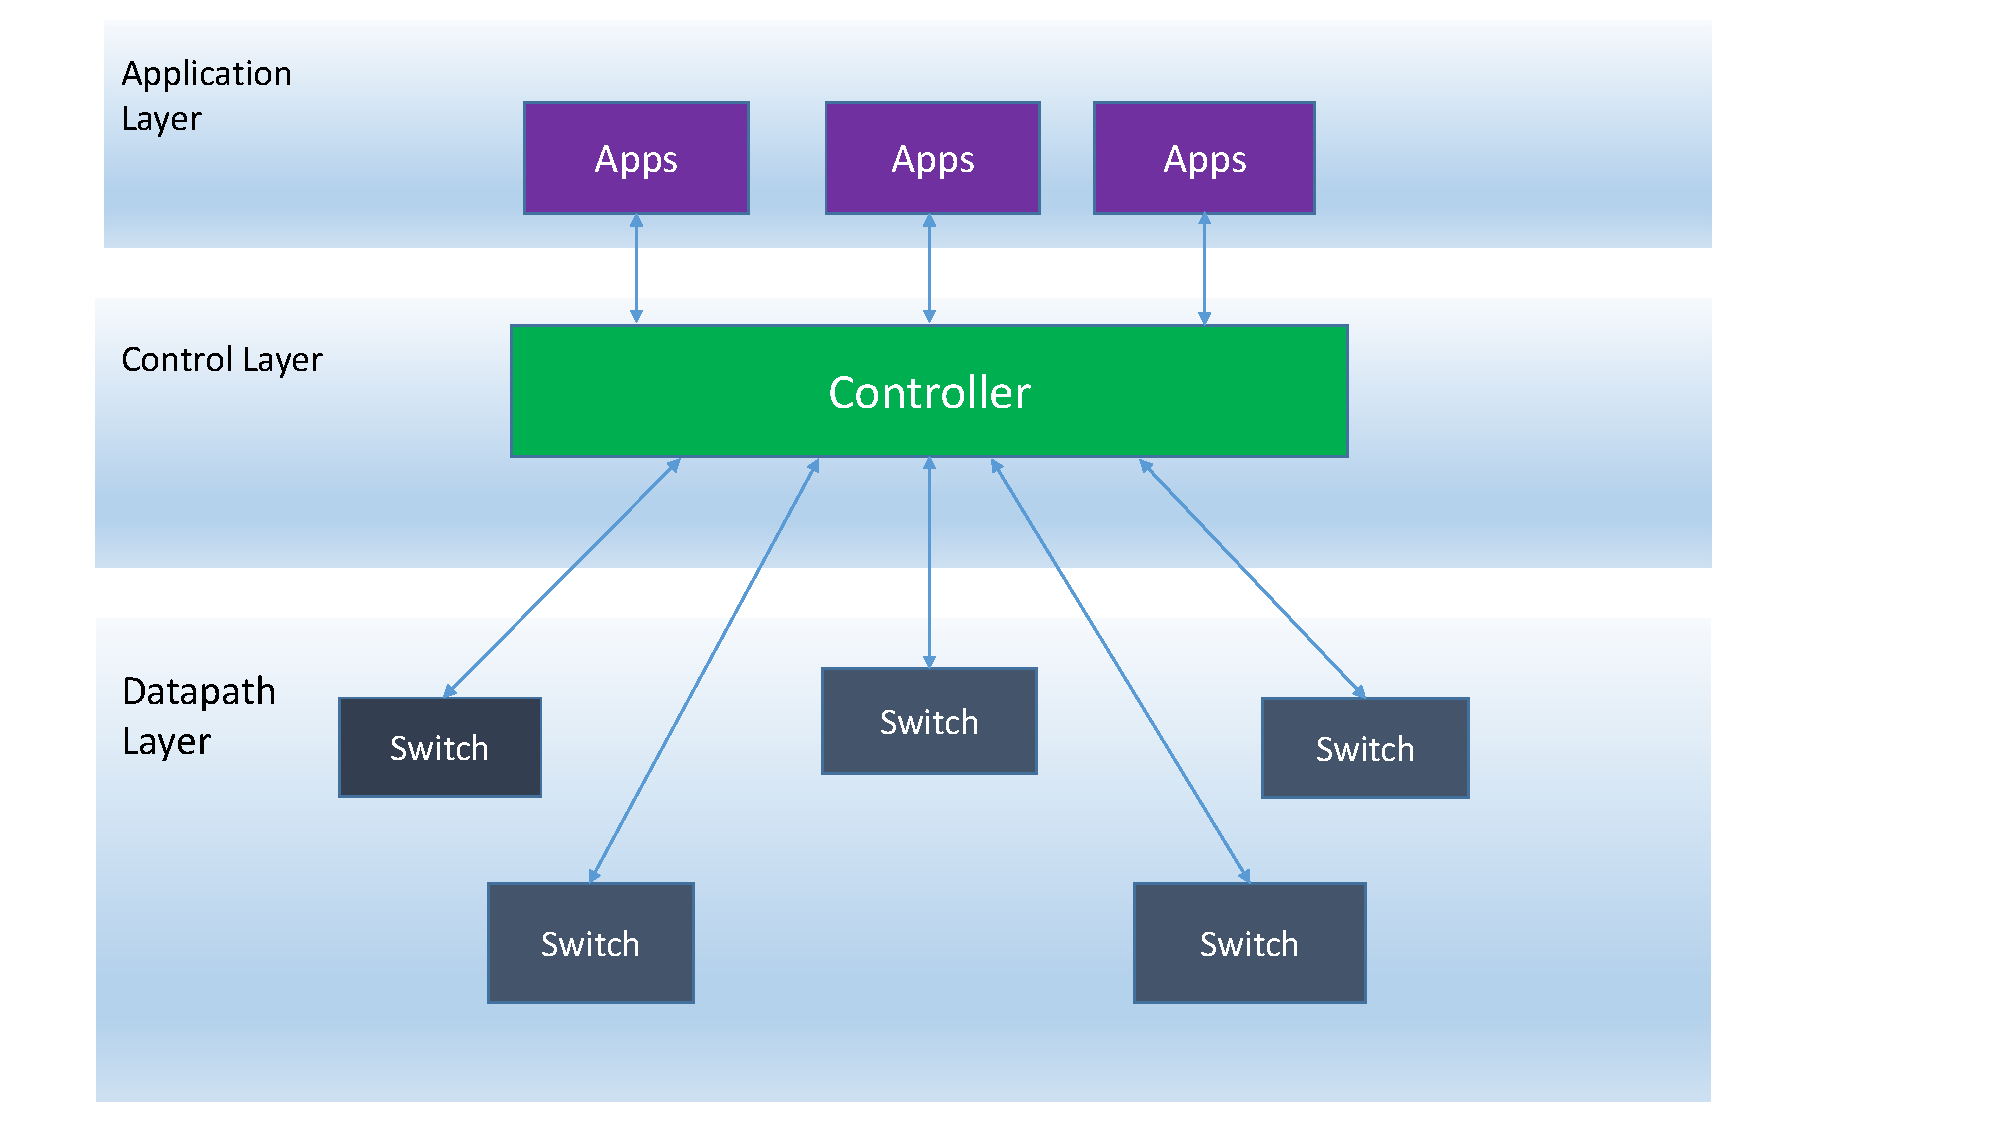
\includegraphics[width=1\textwidth]{figures/SDN.pdf}
  \caption{Overview of Software Defined Networking Architecture}
  \label{fig:SDN}
\end{figure}

\section{Software Defined Networking.}
Network reconfigurability is a major challenge in the networking industry. The explosion of mobile devices and cloud services have necessiated the need for on-demand installation of services and reconfiguration of flow rules according to changing traffic patterns. In addition, network elements like routers and switches have their own unique interfaces and as such management of network components is a source of concern for network operators. As network grows, this complexity increases exponentially and rolling out new services becomes a tedious and complicated proces.

Software Defined Networking (SDN) is an architecture which addresses these challenges by decoupling the control and forwarding functions. This enforces abstraction of underlying implementation and enables applications or network services to be developed using the abstractions as shown in Figure~\ref{fig:SDN}. This simple and elegant design also provides applications a centralized view of the network. As a result, it has sparked tremendous research interest in providing a scalable, secure and programmatic approach towards the challenges discussed above. While SDN is a revolutionary approach, it is still mainly geared towards wired networks. The wireless networks have not recieved much attention in this regard. Through \aetherflow, we provide a protocol independent approach for bringing wireless into SDN model. In this thesis, we go a step further and provide a mechanism for dynamic radio resource management to obtain true network visibility in a heterogeneous network.     

\begin{figure}[t]
  \centering
  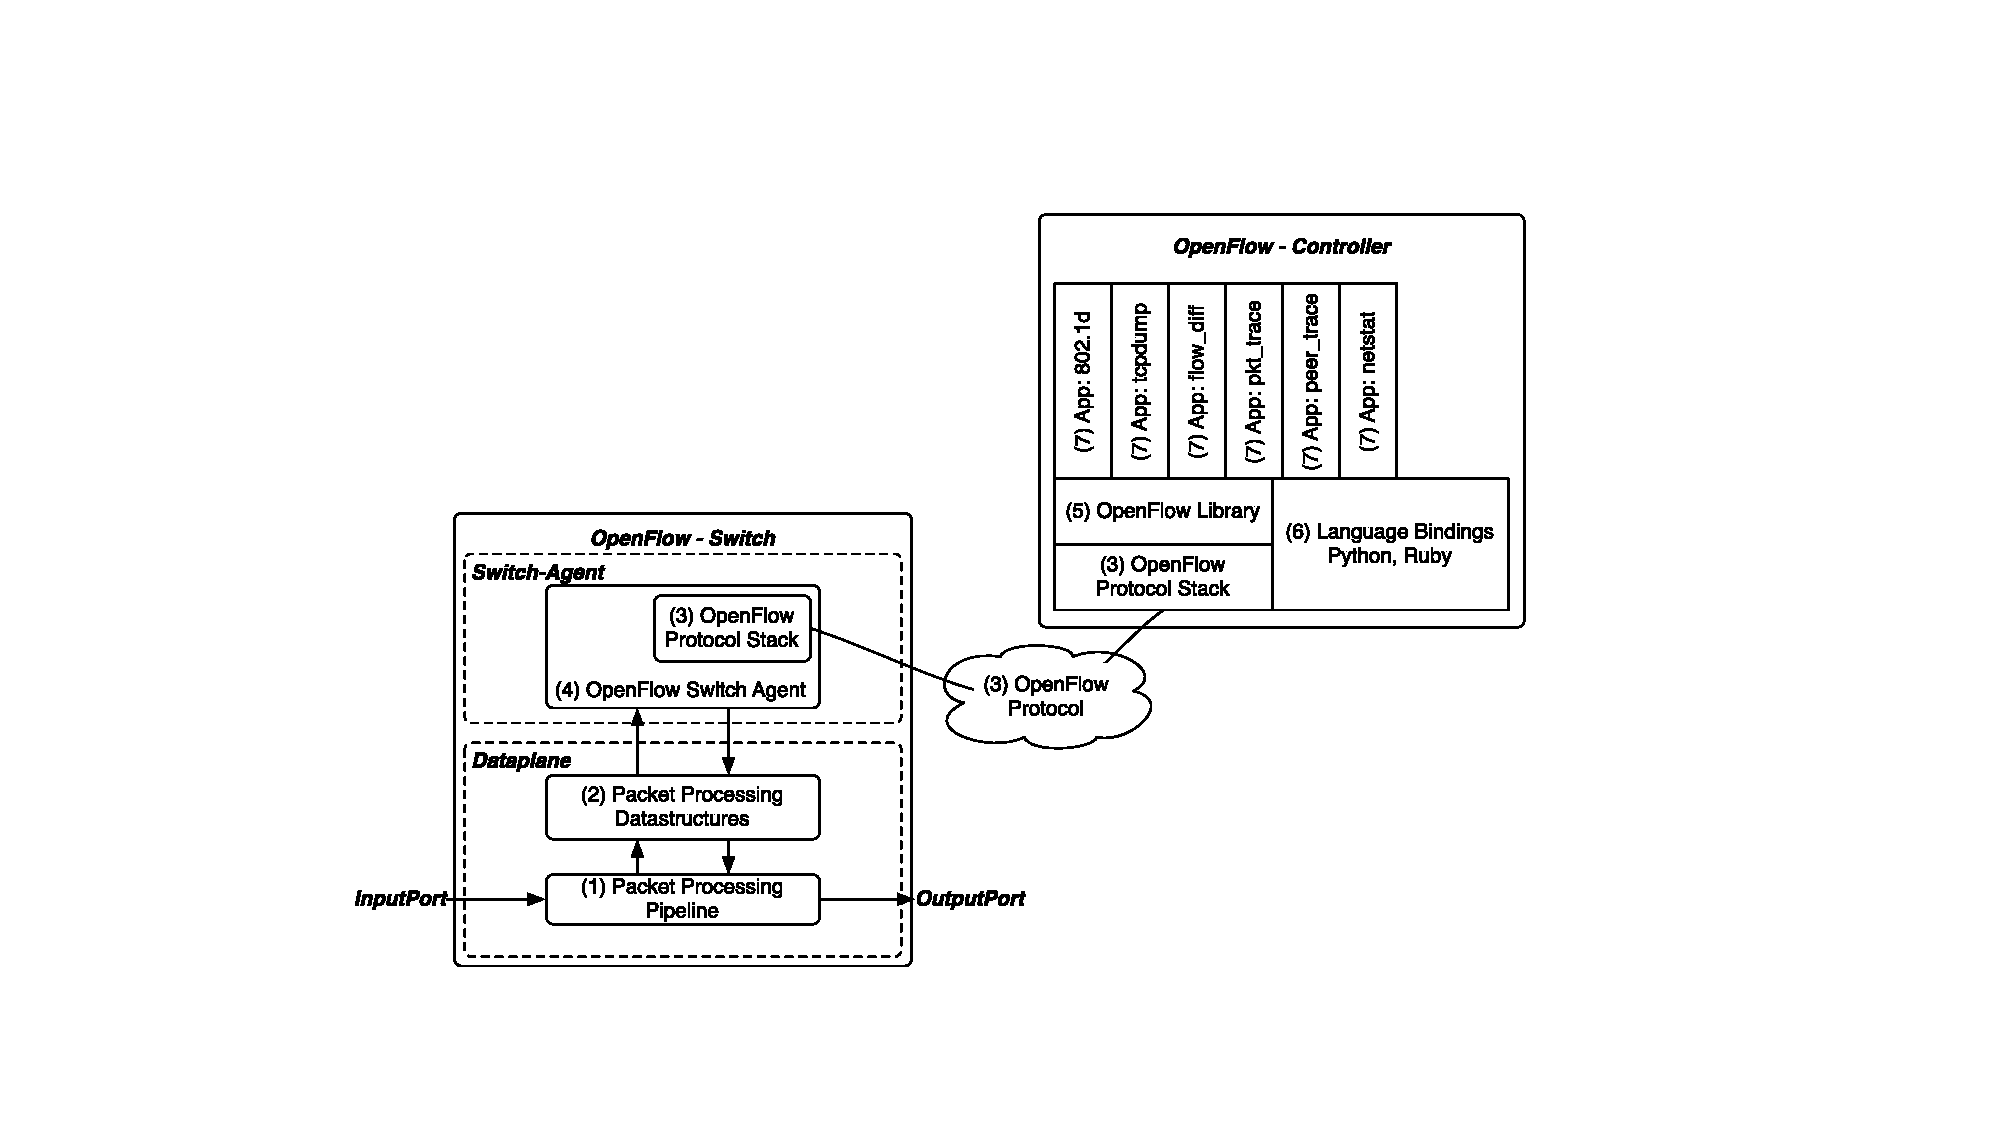
\includegraphics[width=1.5\textwidth]{figures/OpenFlow.pdf}
  \caption{SDN Ecosystem with OpenFlow protocol}
  \label{fig:OpenFlow}
\end{figure}
\section{OpenFlow.}
OpenFlow is an open standard, that began as research project, which allows researchers to experiment with innovative protocols on network switches, without the requirement of exposure to thier internal implementations. OpenFlow\cite{openflow} builds upon the control and data plane abstractions envisioned in the SDN framework, to provide a well defined communication protocol between the two planes as well as a flow table abstraction. Each entry in a flowtable is composed of a number of fields for a packet to match upon, along with a set of associated instructions; each instruction involves performing some actions on a packet or modification of the pipeline processing in the form of allowing packets to be sent to other tables for processing. The OpenFlow communication protocol allows the centralized controller to interact with the switches so that the controller can add, delete or modify the flow table entries to perform certain processing actions. The protocol runs over TCP/TLS (Transport Layer Security) connection so that the communication remains secured and prevent unwanted intrusion which can compromise the security of the entire network. In order for a switch to understand controller's commands, the switch vendors implement a switch agent and in this manner the implementation detail is abstracted out from the controller's point of view. This abstraction paradigm helps in development of sophisticated applications which can leverage the OpenFlow primitivies, to configure the data plane as well as listen for specific events, thereby enabling an asynchronous programmming model. This OpenFlow enabled SDN ecosystem opens the door for various network innovations and in this thesis, we leverage this model to implement a programmable control plane for radio resource management using Software Defined Radio (SDR). An overview of the current SDN ecosystem is presented in Figure~\ref{fig:OpenFlow}.     

\begin{figure}[t]
  \centering
  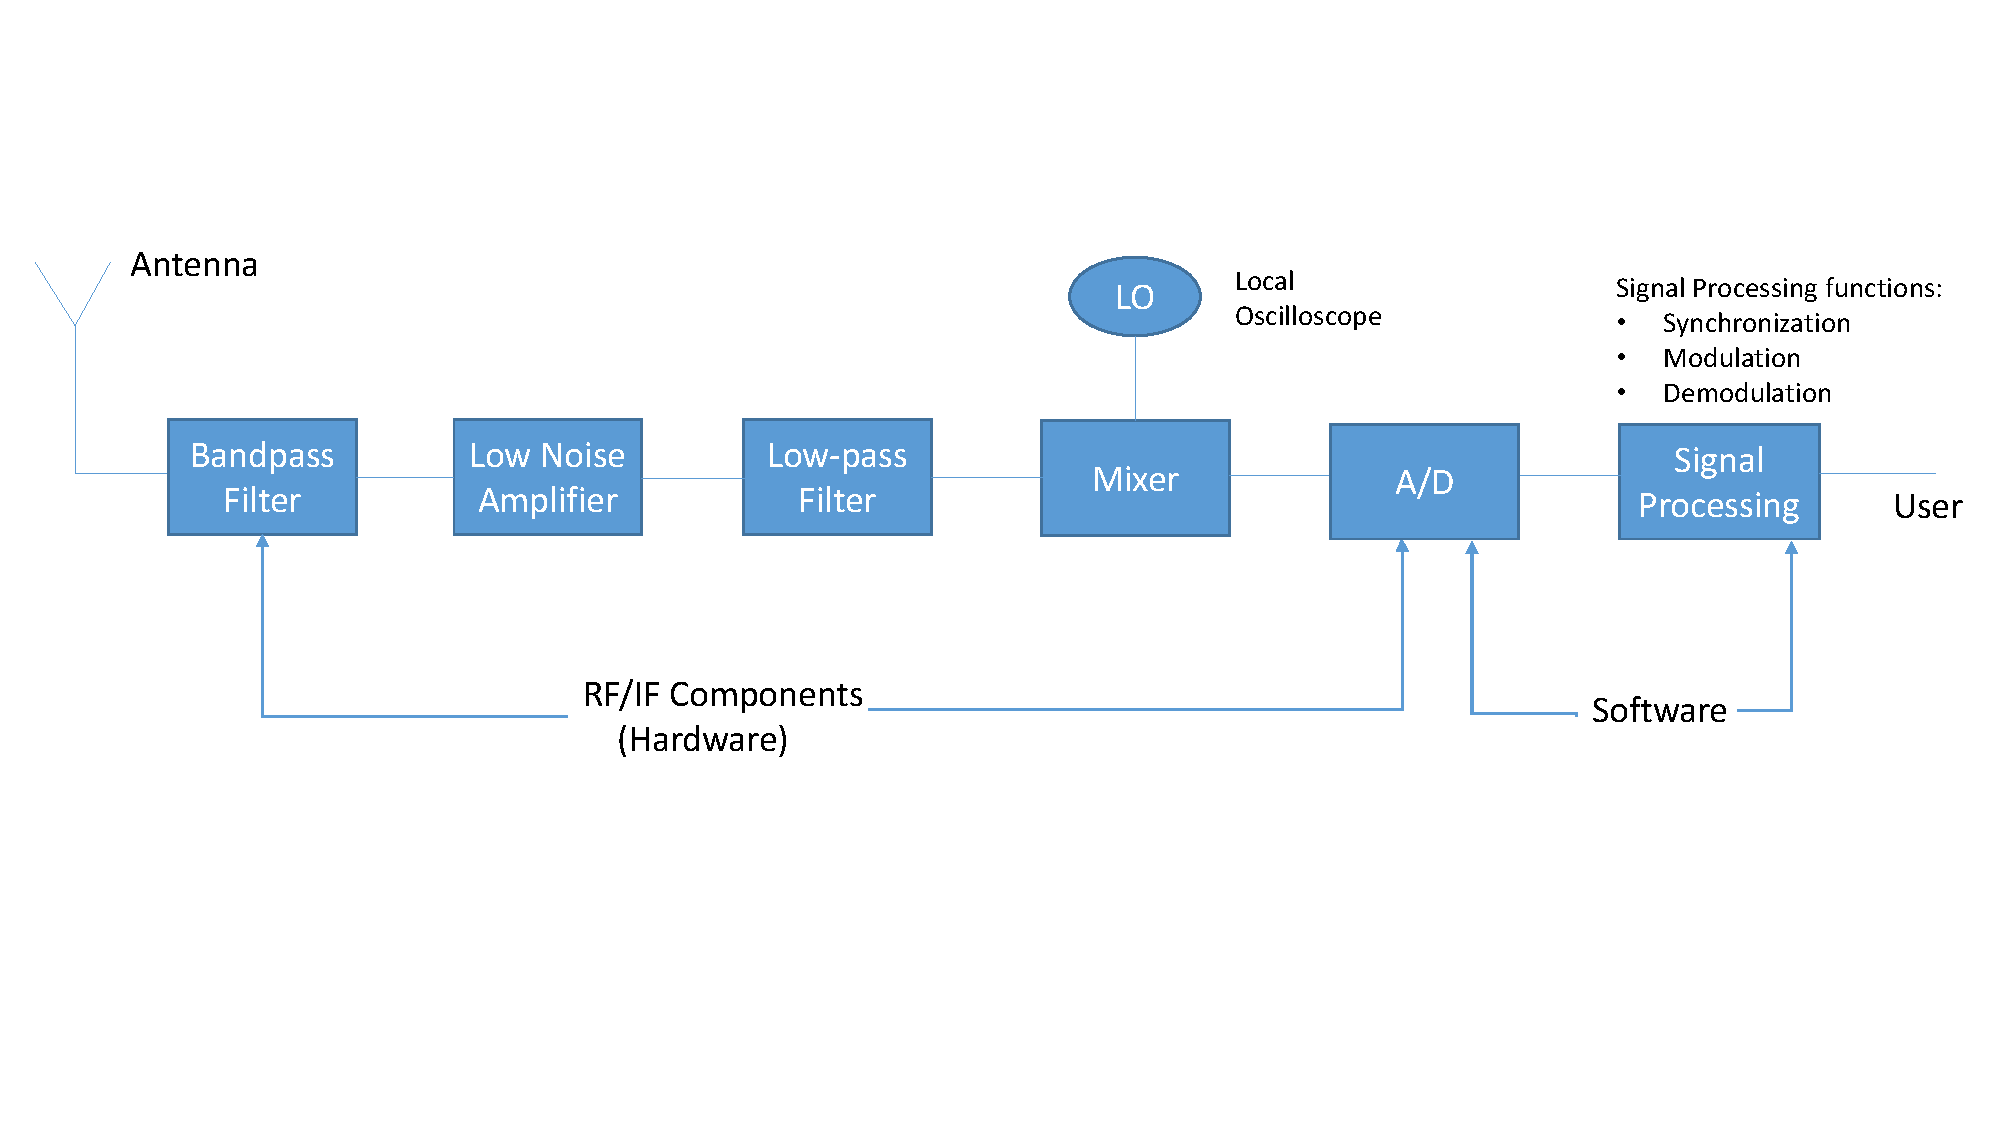
\includegraphics[width=1\textwidth]{figures/SDR.pdf}
  \caption{Components of Software Defined Radio (SDR)}
  \label{fig:SDR}
\end{figure}
\section{Software Defined Radio (SDR).}
Most of the wireless protocols in use today are implemented in hardware. With the ever increasing number of protocols to be supported and their diverse requirements, it has become apparent that a programmable environment for hardware is the need of the hour. This requirement gave rise to the concept of Software Defined Radio (SDR). SDR is a communications system in which various hardware-centric features such as filters, modulators/demodulators and other signal processing blocks are implemented in software, rather than hardware, as shown in Figure~\ref{fig:SDR}. This is a powerful concept as this design offers high flexibility and runtime reconfiguration. This methodology also has the advantage that the radio can be configured to support various physical-layer protocols based on software, eliminating the need of custom, inflexible, and expensive hardware implementations. This property of reconfigurability is an important feature for various dynamic systems utilizing cognitive radio functionalities.As a result there is a significant interest among researchers and industry alike to make SDR a reality for network operators and end users. In this thesis, we use the programmable feature of SDR to define new abstractions and expose interfaces so that a network of radios can be controlled using SDN principle. 

\section{GNU Radio framework.}
GNU Radio \cite{gnuradio} is a free and open-source framework that provides signal processing functionality to implement SDRs. The main constituents of the framework are basic blocks which perform distinct signal processing functions. GNU Radio provides great leverage to compose these blocks to synthesize new radio functionality on a general purpose hardware. But the framework alone is not suitable for developing applications to control a network of SDRs. This is because each block exposes its own set of interfaces which does not scale with increasing numbers of radios in the network. In this thesis, we provide uniform interfaces to control and manage these processing block abstractions, so that an application developer does not need to handle every block's unique interface characteristics.


\chapter{\uppercase {Related Work}}
\label{sec:related}
\section{Extension of Wireless LAN} 

The interest for extending WLAN capabilities has been a community goal for a long time, but traditional methods have certain constraints. For example, the approaches reported in \cite{murty10dyson,shrivastava09centaur} require modifications to the mobile clients (referred to as \emph{mobile stations} in the Wi-Fi standard), which makes those approaches hard to deploy and test.

A recent technical report by the Open Networking Foundation (ONF) \cite{onf13enabled} identified the challenges of mobile  networks, such as scalability, management, flexibility and cost, and provided a brief discussion of how SDN solutions can address these issues in few specific scenarios. A working group of Open Networking Foundation, Wireless \& Mobile Working Group (WMWG), has been focusing on devising new SDN architecture for wireless use cases of different types \cite{onf-wmwg:proposal}. However, to the best of our knowledge no concrete solutions were proposed by either ONF or WMWG up to now.

Several previous works presented systems that use OpenFlow extensions to achieve specific goals in wireless networks. In particular, OpenRoad \cite{yap10openroads, yap10blueprint, yap09stanford} proposes to use the OpenFlow framework as a research platform for Wi-Fi and Wi-MAX systems. The platform supports  slicing and virtualization of network resources, allowing different experimental  services to run at the same time. SoftCell \cite{jin13softcell} focused on LTE networks and proposed to integrate SDN framework into the LTE core network architecture.  The objective of \aetherflow is to design data plane control interfaces for wireless ports, which is different from these projects.

Other attempts to apply SDN to IEEE~802.11 networks include Odin~\cite{suresh12odin} and OpenSDWN~\cite{schulz15opensdwn}. They provide certain wireless interface control and configuration capabilities to the SDN controller. In these solutions, virtual access points and associated device contexts are created for each individual mobile device, and move across access points when the client handoff occurs. Such type of framework can handle user mobility gracefully, but results in overhead in terms of both computational load and traffic load during handoff, especially in the settings with a large number of clients and high user mobility. \aetherflow offers a set of interfaces that costs less but still supports a wide variety of wireless applications.

In contrast to the existing works, \aetherflow  provides a principled and general definition of wireless abstractions within an existing SDN framework. Our approach only requires incremental modifications to the existing SDN network elements.

\section{Programmatic Wireless Dataplane} 

The idea of providing a programmable wireless data plane has been implemented in~\cite{atomix} and~\cite{openradio}. Both these papers provide modular blocks and focus on real time guarantees for processing signals. But like GNU Radio, they do not provide any logical interface to control a network of such programmable devices. We choose GNU Radio in our design as it provides unlimited flexibility. The paper ~\cite{softran} deals with centralized control of devices but it focuses mainly on LTE networks. Our work is orthogonal to these works as we provide a mechanism for centralized control while making the exposed interfaces protocol independent.
The combination of SDRs and SDN has been introduced for various functionality in ~\cite{cho2014integration, sun2015integrating}, ~\cite{mancuso2014prototyping}, ~\cite{corbett2014countering} and ~\cite{sdnsdrinsno}. ~\cite{mancuso2014prototyping} deals with creation of testbed for LTE technologies while ~\cite{cho2014integration, sun2015integrating} focuses mainly on integration of SDN and SDR for 4G/5G technology.~\cite{gupta2015labview} describes a SDR model for management of interference in dense heterogeneous networks while ~\cite{corbett2014countering} developed a jamming architecture using SDN and SDR principles. ~\cite{sdnsdrinsno} provides a blueprint for LTE self-organizing networks(SONs) using SDN and SDR principles. These papers provide distinct solutions for various scenarios but do not provide a generic framework for handling various protocols in a principled manner.

\chapter{\uppercase {OpenFlow Extensions}}
\label{sec:extensions}

\blfootnote{*Reprinted with permission from ``\aetherflow: Principled Wireless Support in SDN" published in CoolSDN '15 ~\cite{aetherflow}, and ``\crossflow: A Cross-layer Architecture for SDR using SDN principles" published in IEEE NFV-SDN '15 \copyright 2015 IEEE ~\cite{crossflow}.}

In our previous work, we derived a generalized SDN abstractions model, called
TinyNBI \cite{Casey:14}, from the OpenFlow specifications \cite{openflow}.
In TinyNBI, the OpenFlow data plane is composed of
several elements. The data plane elements and their structural relationships are
depicted as UML diagram in Figure~\ref{fig:data_model}. TinyNBI model provides a 
clean low-level interpretation of the core OpenFlow abstractions and supports 
development of higher layer abstractions through refinement or extension.
The model is primarily based on the notion of resources shared across a
data plane. 

% A data plane receives packets from a set of different ports, and
% forwards those to a pipeline, defined largely by table lookups and their
% associated actions, for processing and forwarding.

\begin{figure}[t]
  \centering
  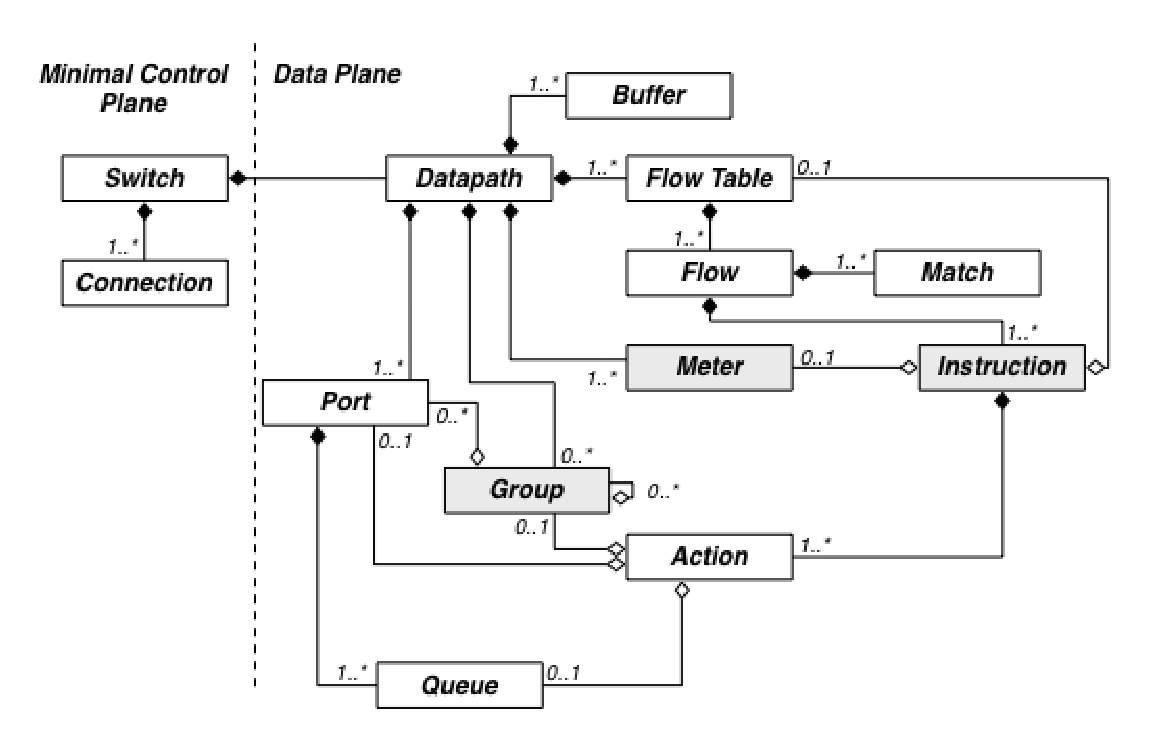
\includegraphics[scale=0.64]{figures/data_model.pdf}
  \caption[UML diagram of OpenFlow data model]{A UML diagram of OpenFlow data model. Each box represents a data
  plane element and the lines show the dependencies relationship among the
  elements.}{[Reprinted\space from\space \textsuperscript{\cite{flowgrammable}}]}
  \label{fig:data_model}
\end{figure}

\begin{figure}[t]
  \centering
  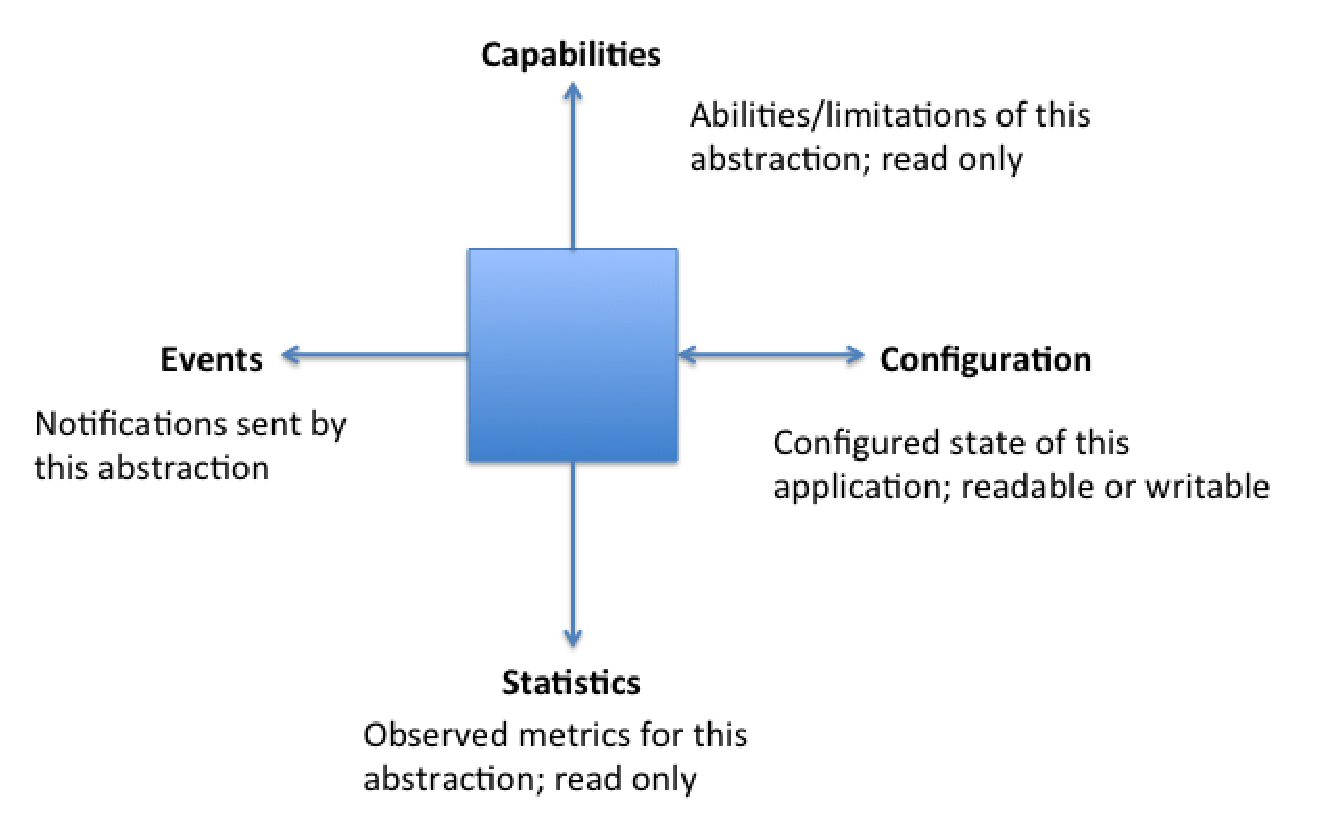
\includegraphics[scale=0.64]{figures/abstraction.pdf}
  \caption{OpenFlow interfaces abstraction.}
  \label{fig:abstraction}
\end{figure}

In the TinyNBI model, each component exposes four types of interfaces:
capabilities, configuration, statistics and events.  These interfaces and their
information flow directions are conceptually depicted in
Figure~\ref{fig:abstraction}.

\textbf{Capabilities.} Not every switch provides the same level of
support for e.g., matching on protocol fields. Each component in the
model must provide a facility that allows a controller to discover the
set of operations supported by the device.

\textbf{Configuration.} Each OpenFlow data model element has some
configurable parameters that can be modified during switch operation.
The configuration interfaces are used to modify state and behavior of the data
model element. 

\textbf{Statistics.}  OpenFlow switches gather statistical information
via counters such as the numbers of bytes received and transferred over a
port. Statistics interfaces provide the controller with access to the current
state and values of these counters. 

\textbf{Events.} The events interface reports to the controller certain
types of events that occur during switch operation. 


%\footnotetext{Courtesy: flowgrammable.org}

\section{\aetherflow Data Plane Abstractions}


In order to support wireless networks, we refine the notion of ports from
the TinyNBI SDN model. The SDN model already has a distinction between
physical and logical ports. A \emph{physical port} corresponds to an actual
interface (e.g., Ethernet card), whereas a \emph{logical port} is typically
defined by software. Logical ports are often used for protocol
tunneling and link aggregation.

To support wireless SDN controllers we introduce new types of both physical
and logical ports. \aetherflow introduces wireless physical port
corresponding to an IEEE~802.11 (commonly known as WiFi) radio interface.
This allows controllers to query and configure the physical device over
which packets are sent and received.

Because a single 802.11 radio interface can support multiple simultaneous
wireless access points (APs), \aetherflow also introduces wireless
logical port. Each wireless logical port is associated with its underlying
physical port.

For packet processing, whenever a packet from a wireless AP is
processed, its metadata records its \emph{input port} as the logical port
for the AP and its \emph{input physical port} as the physical port the AP is
created on. The frames received on
the wireless interface are adapted into regular Ethernet frames for pipeline
processing, meaning that we
do not have to define any new protocol matching features for 802.11 MAC frame
fields. This also allows an existing SDN implementation to compose
wireless logical ports into link aggregation ports or various forms of
tunnels.
% 
% Note that we could readily extend the matching capabilities for table
% abstractions to support frames received directly from a physical port.
% We reserve this for future work.

The new data plane elements (wireless ports) defined in \aetherflow expose to
the controller a set of control interfaces, categorized in the same way as the
TinyNBI model, which are described as below.

\textbf{Capabilities.}
\aetherflow allows the controller to query and obtain the capabilities of the
radio interfaces of an AP. The supported capabilities information for wireless
physical port includes 
% contains:
% \begin{itemize}
%   \item Wireless physical port: 
    (i) IEEE~802.11 version; 
    (ii) channels; 
    (iii) transmission power; 
    (iv) encryption and key management methods; 
    (v) maximum number of APs supported.
%\end{itemize}
\aetherflow does not define capabilities interface for wireless logical port.

\textbf{Configuration.}
An OpenFlow controller can use \aetherflow messages to create or remove AP and
dynamically 
(re)configure the following properties of an AP:
\begin{itemize}
  \item Wireless physical port: 
     (i) IEEE~802.11 version; 
    (ii) channel; 
    (iii) transmission power. 

  \item Wireless logical port: 
    (i) SSID; 
    (ii) BSSID; 
    (iii) encryption and key management method.
\end{itemize}

In addition, \aetherflow allows the controller to change the state of mobile
stations associated with it, e.g., drop a station. Any new configuration to an
AP is immediately applied. The configuration interfaces provide
a high degree of programmability to applications that require these parameters 
to be adjusted during network operation.

\textbf{Events.}
  An SDN controller can receive MAC layer events related to a mobile station. 
  \aetherflow currently supports the following types of
  events for wireless logical port:
  % \begin{itemize}
  %    \item Wireless logical port: 
      (i) probe; 
      (ii) authentication; 
      (iii) deauthentication; 
      (iv) association; 
      (v) reassociation; 
      (vi) disassociation; 
      (vii) authorization.
  %\end{itemize}
\aetherflow does not define any event interface for wireless physical port.
 % No event interface is defined for wireless physical port.

  The events occur when AP receives the corresponding 802.11 management frames.
  With these events reported, the controller can keep track of the 802.11 state
  of all the mobile stations communicating with the APs under control. 

\textbf{Statistics.}
  An SDN controller can query the statistics of each physical wireless
  port and its associated logical ports. For a wireless logical port the following types
  of statistics are supported: 
  % \begin{itemize}
  %    \item Wireless logical port: 
      (i) number of packets sent and received; 
      (ii) number of bytes sent and received; 
      (iii) number of retries;
      (iv) number of retry failures; 
      (v) current signal strength of a station; 
      (vi) average signal strength of a station; 
      (vii) connection duration of a station.
 %   \item Wireless physical port:
For wireless physical port the set of supported statistics is identical to that supported by the OpenFlow protocol. 
% 
% 
% \aetherflow  from the OpenFlow statistics interface model.
 % \end{itemize}


\section{\aetherflow Messages}
To implement \aetherflow in the framework of OpenFlow, we use experimenter
messages provided in OpenFlow protocol to carry \aetherflow messages. In the current
version, nine messages are defined in \aetherflow:
\begin{itemize}
\item Event report message -- notify controller of events.
\item Logical port statistics request/reply -- request and reply of current 
      statistics from a logical port.
\item Physical port configuration request -- modify the configuration of a
      physical port.
\item Logical port configuration request -- modify the configuration of a
      logical port.
\item Physical port capabilities request/reply -- request and reply of 
      capabilities of a physical port.
\item Drop station -- force a mobile station to disassociate.
\item Error message -- customize error reporting for wireless.
\end{itemize}
% The detailed definitions of the messages are omitted due to space limit.
%  For the counters, the switch keeps one counter for each station and each type
%  of statistics. The counter may be turned on or off by the controller. If
%  turned on, the counter gets updated when a corresponding event happens. Signal
%  strength of the client is measured and updated when a frame is received from
%  the corresponding station. Connection state refers to the state of the mobile
%  station in the 802.11 MLME state machine (unauthenticated/unassociated,
%  authenticated/unassociated, authenticated/associated/pending RSN
%  authentication and authenticated/associated).

\section{\crossflow Data Plane Abstractions}

%\begin{figure}[t]
%  \centering
%  \includegraphics[width=0.48\textwidth]{figures/Interfaces.pdf
%  \caption{Interface model for wireless radio port abstraction with two processing blocks: Sink and Modulators}
%  \label{fig:interface}
%\end{figure}

\begin{figure}[t]
  \centering
  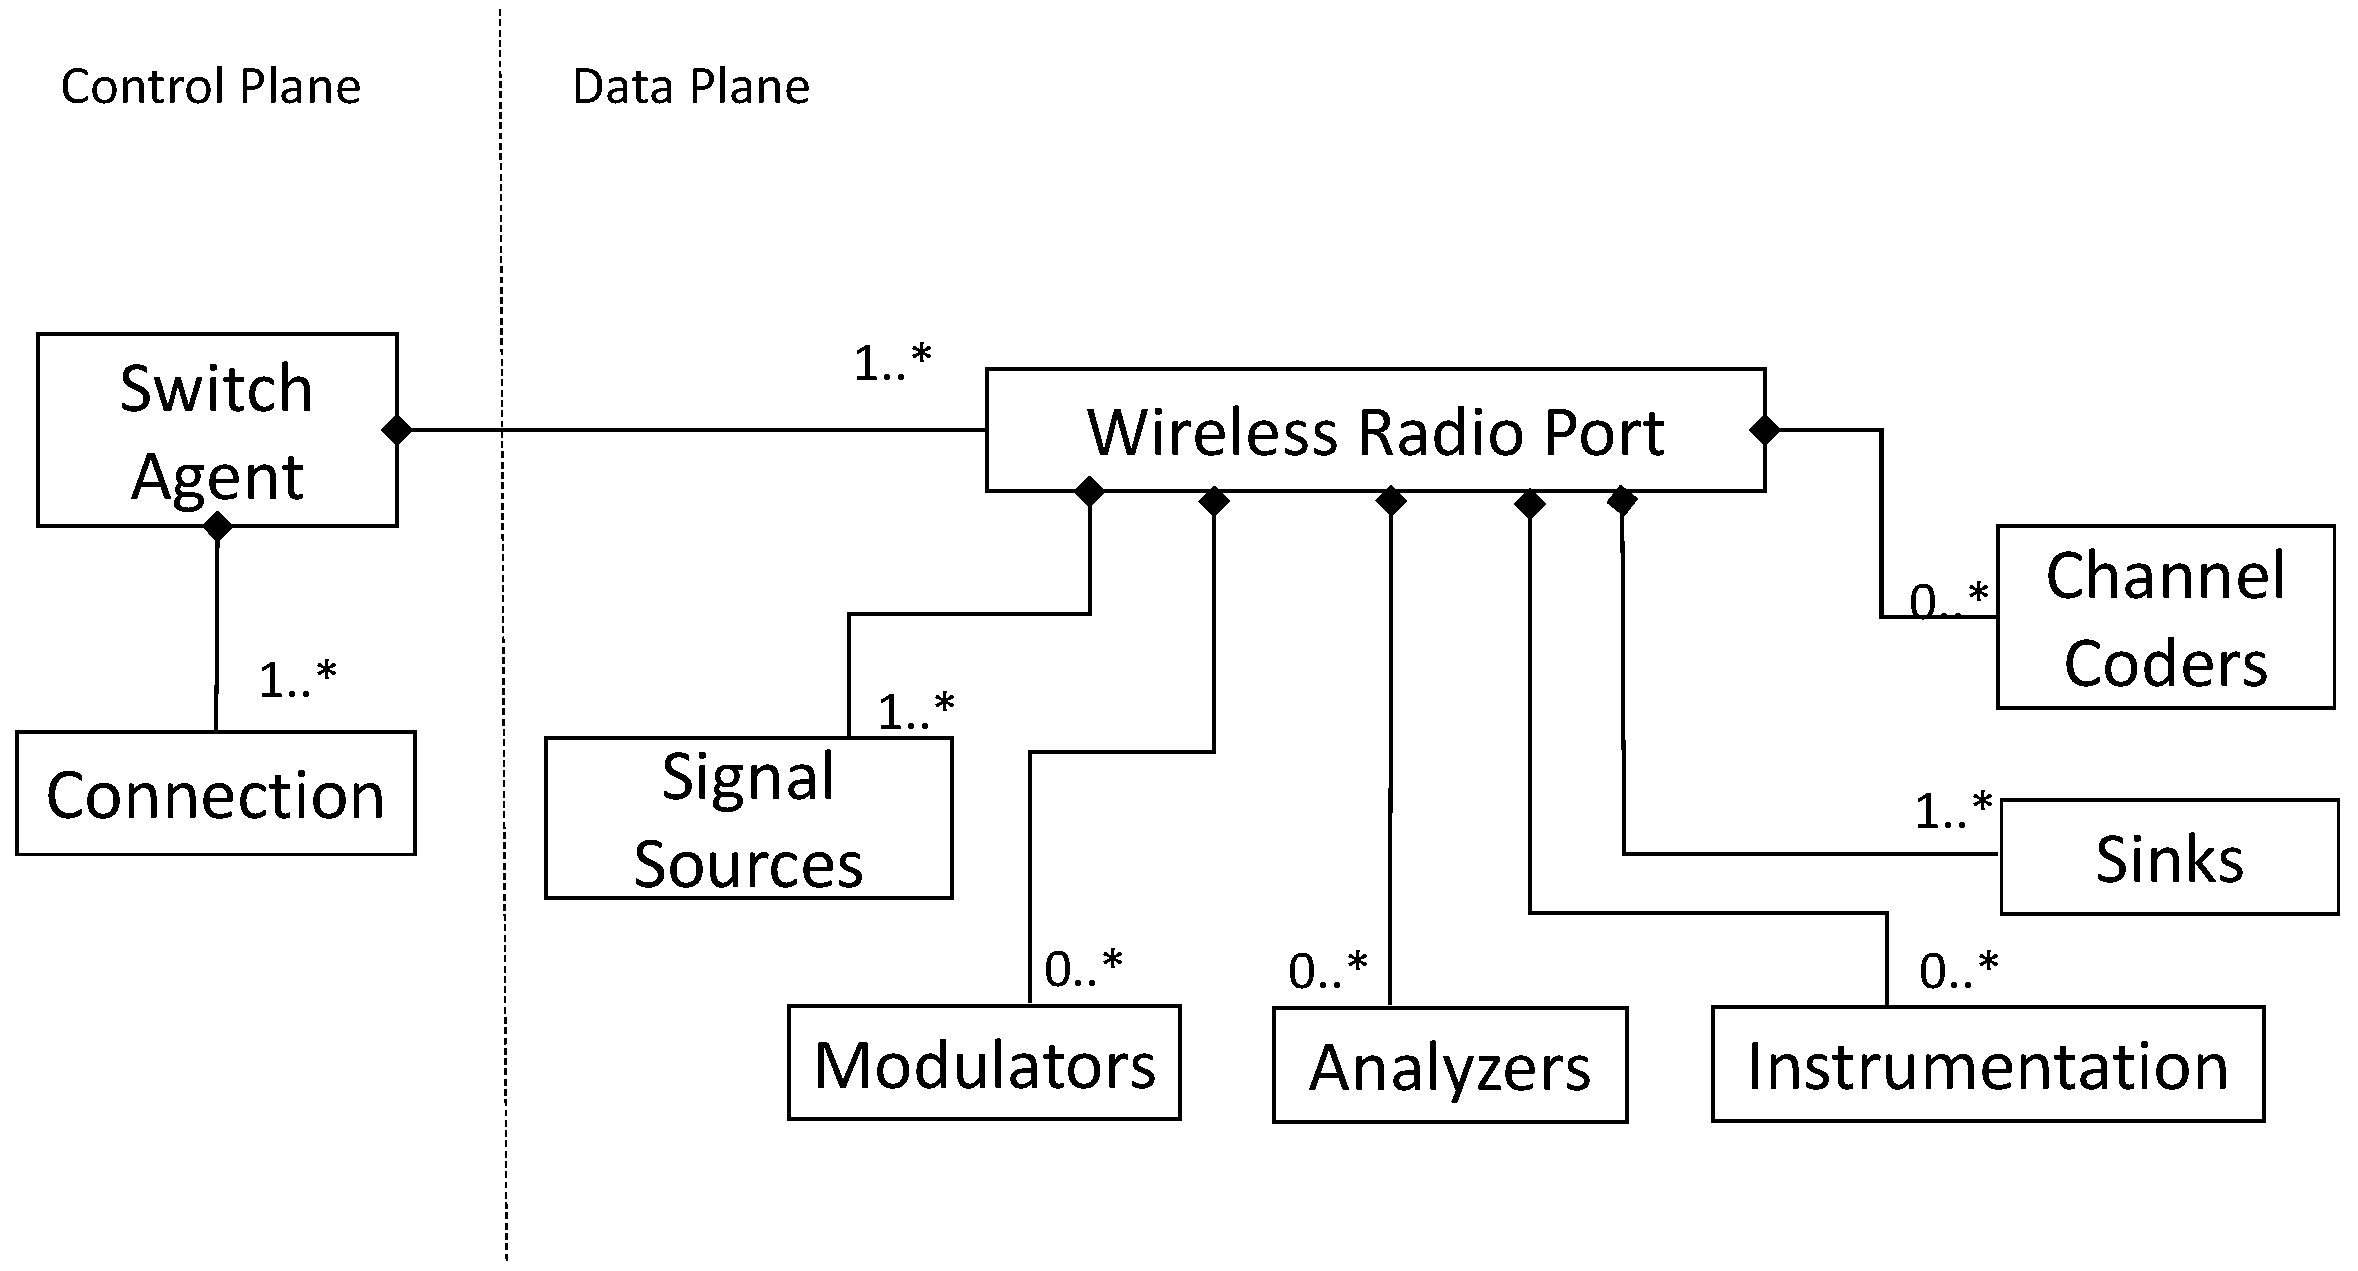
\includegraphics[width=0.8\textwidth]{figures/UML.pdf}
  \caption{UML diagram of \crossflow model.}
  \label{fig:uml}
\end{figure}

%\begin{figure*}
%  \centering
%  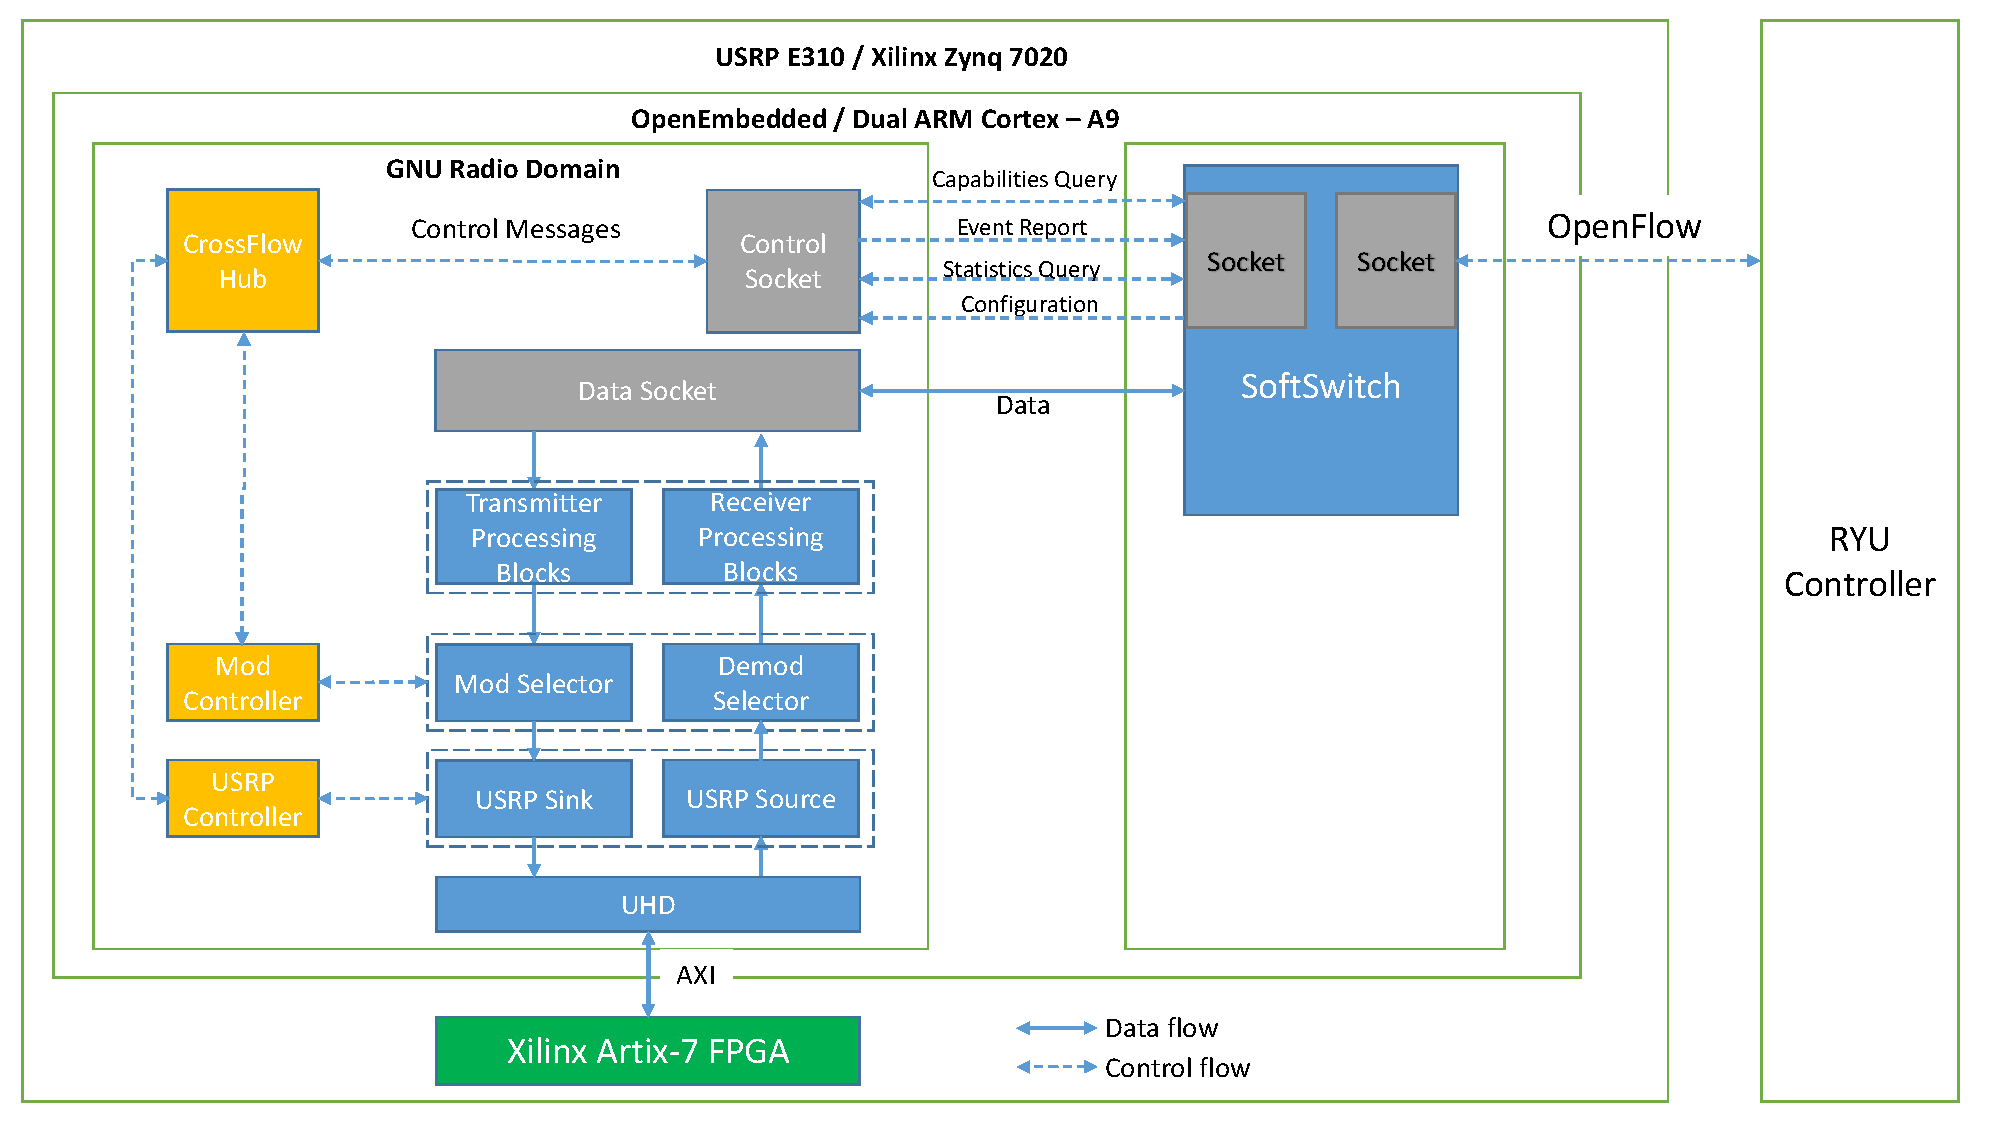
\includegraphics[width=0.8\textwidth]{figures/new.pdf}
%  \caption{Implementation of \crossflow}
%  \label{fig:message_block}
%\end{figure*}

We extend the data model proposed in \cite{Casey:14} to create an abstraction model for the \crossflow framework, which is displayed in Figure~\ref{fig:uml}. We build upon the \emph{radio physical port} concept proposed in \cite{aetherflow} to create a new layer of abstractions, which we refer to as the \emph{wireless radio port} in this paper. This layer of abstractions exhibits a composition or \emph{has-a} relationship with the \emph{wireless radio port} abstraction (i.e., ``the wireless radio port \emph{has a} sink, modulator, or channel coder). This means that the blocks of this layer are the objects or members that comprise the \emph{wireless radio port}. These blocks are derived from the most commonly used processing blocks in GNU Radio~\cite{gnuradio}. This abstract wireless radio port model serves the following design vision:

\begin{itemize}
\item It allows visibility into the signal processing blocks from an application point of view, without going into implementation details.
\item It allows for the development of an event driven framework for radio operation.
\item It allows composition of blocks to implement new functionality, as this decision is handled by the higher \emph{radio physical port} abstraction. The application simply specifies the blocks to be connected for a specific wireless port instance and the internal framework handles the implementation.
\end{itemize}

In our current design, we focus on the first point of changing and quering the parameters of blocks at runtime. We assume that the number of blocks is fixed and the blocks can be connected in a consistent manner. In order to change parameters, the application needs to send \emph{\big \langle command,value\big \rangle} tuple in a message. For query and receive event responses, it registers for events for each block and during an event, appropriate callbacks are invoked. This ability to register for events is important so that a centralized controller can receive events asyncronously and implement a reactive model for its operations.
    
One of the main requirements of the \crossflow model is that each abstraction should implement four types of interfaces as proposed in \cite{Casey:14}, namely: capabilities, configuration, statistics and events. The interface model for \crossflow provides the interfaces for a wireless radio port abstraction with only two processing blocks, \emph{Sink} and \emph{Modulators}. The Sink abstraction allows the controller to manage the signal sinks which can be a USRP device, file or a socket, while the Modulators abstraction allows management of modulation schemes (e.g., BPSK, QPSK, and 8PSK).

The interfaces for \emph{Sink} and \emph{Modulators} are categorized as follows:

%\textbf{Capabilities.}
\textbf{Sink.}
\begin{itemize}
\item \textbf{Capabilities}: The interface allows the controller to query the capabilities of sinks such as:
    (i)  Type of sink (USRP, socket, etc.);
    (ii) Channels supported; 
    (iii) Center Frequency; and
    (iv) IP address. 
\item \textbf{Configuration}: The interface allows the controller to configure properties of signal sinks such as:
    (i) Gain;
    (ii) Frequency, and
    (iii) Sample rate.
\item \textbf{Statistics}: The interface allows the controller to gather statistics for sinks such as:
    (i) Received Signal Strength Indicator (RSSI) and 
    (ii) Temperature on-board.
\item \textbf{Events}: The interface allows the controller to take decisions based upon events in a sink such as:
    (i) Low or high RSSI and
    (ii) Low or high on-board temperature.
\end{itemize}

\textbf{Modulators.}
\begin{itemize}
\item \textbf{Capabilities}: The interface allows the controller to query the properties of the modulator block such as:
    (i) Modulations supported;
    (ii) Current samples/symbol; and
    (iii) Gray code.
\item \textbf{Configuration}: The interface allows the controller to configure properties of the modulator block such as:
    (i) Choice of modulation scheme (e.g. BPSK, QPSK and 8PSK);
    (ii) Samples/symbol; and
    (iii) Use of a Gray code.
\item \textbf{Statistics}: The interface allows the controller to gather statistics for the modulator block such as:
    (i) Signal to Noise Ratio (SNR) and 
    (ii) Bit Error Rate (BER).
\item \textbf{Events}: The interface allows the controller to take decisions based upon events in the modulator block such as:
    (i) Low or high SNR and
    (ii) Low or high BER.
\end{itemize}

\section{\crossflow Message Extensions}
\label{sec:messages}
  		  
\crossflow uses SDN design principles to control a network of configurable SDRs. As such, to enable control plane interactions between the SDN controller and the SDR, we had two options: either we could have implemented our own control protocol to enable their interactions or extend the existing OpenFlow \cite{openflow} framework. This is because OpenFlow does not natively support wireless features. In order to enable a cleaner implementation, we decided to extend OpenFlow by using experimenter messages within the OpenFlow protocol, similar to \aetherflow. Experimenter messages are a part of the standard OpenFlow protocol which provides a mechanism for vendors to include propriety information within the protcol. This provides us with two advantages:
\begin{itemize}
\item We do not need to implement a new protocol for control and data plane interactions.
\item As we are using experimenter messages to carry \crossflow messages, the SDN controller does not need to perform special handling for these messages. This enables the controller to remain independent of the underlying devices and hence it can handle both wired and wireless devices.
\end{itemize}
In the current version, we define three messages in \crossflow:
\begin{itemize}
\item Configuration message request - Request for modification of parameters like gain, frequency, SNR threshold and modulation scheme.
\item Statistics message request - Request for statistics such as SNR, BER and RSSI.
\item Event message response - Response for events like SNR below threshold and low BER.
\end {itemize}

\chapter{\uppercase {\aetherflowcap Implementation}}
\label{sec:impl}

\section{Implementation on an AP}


\begin{figure*}[t]
\centering
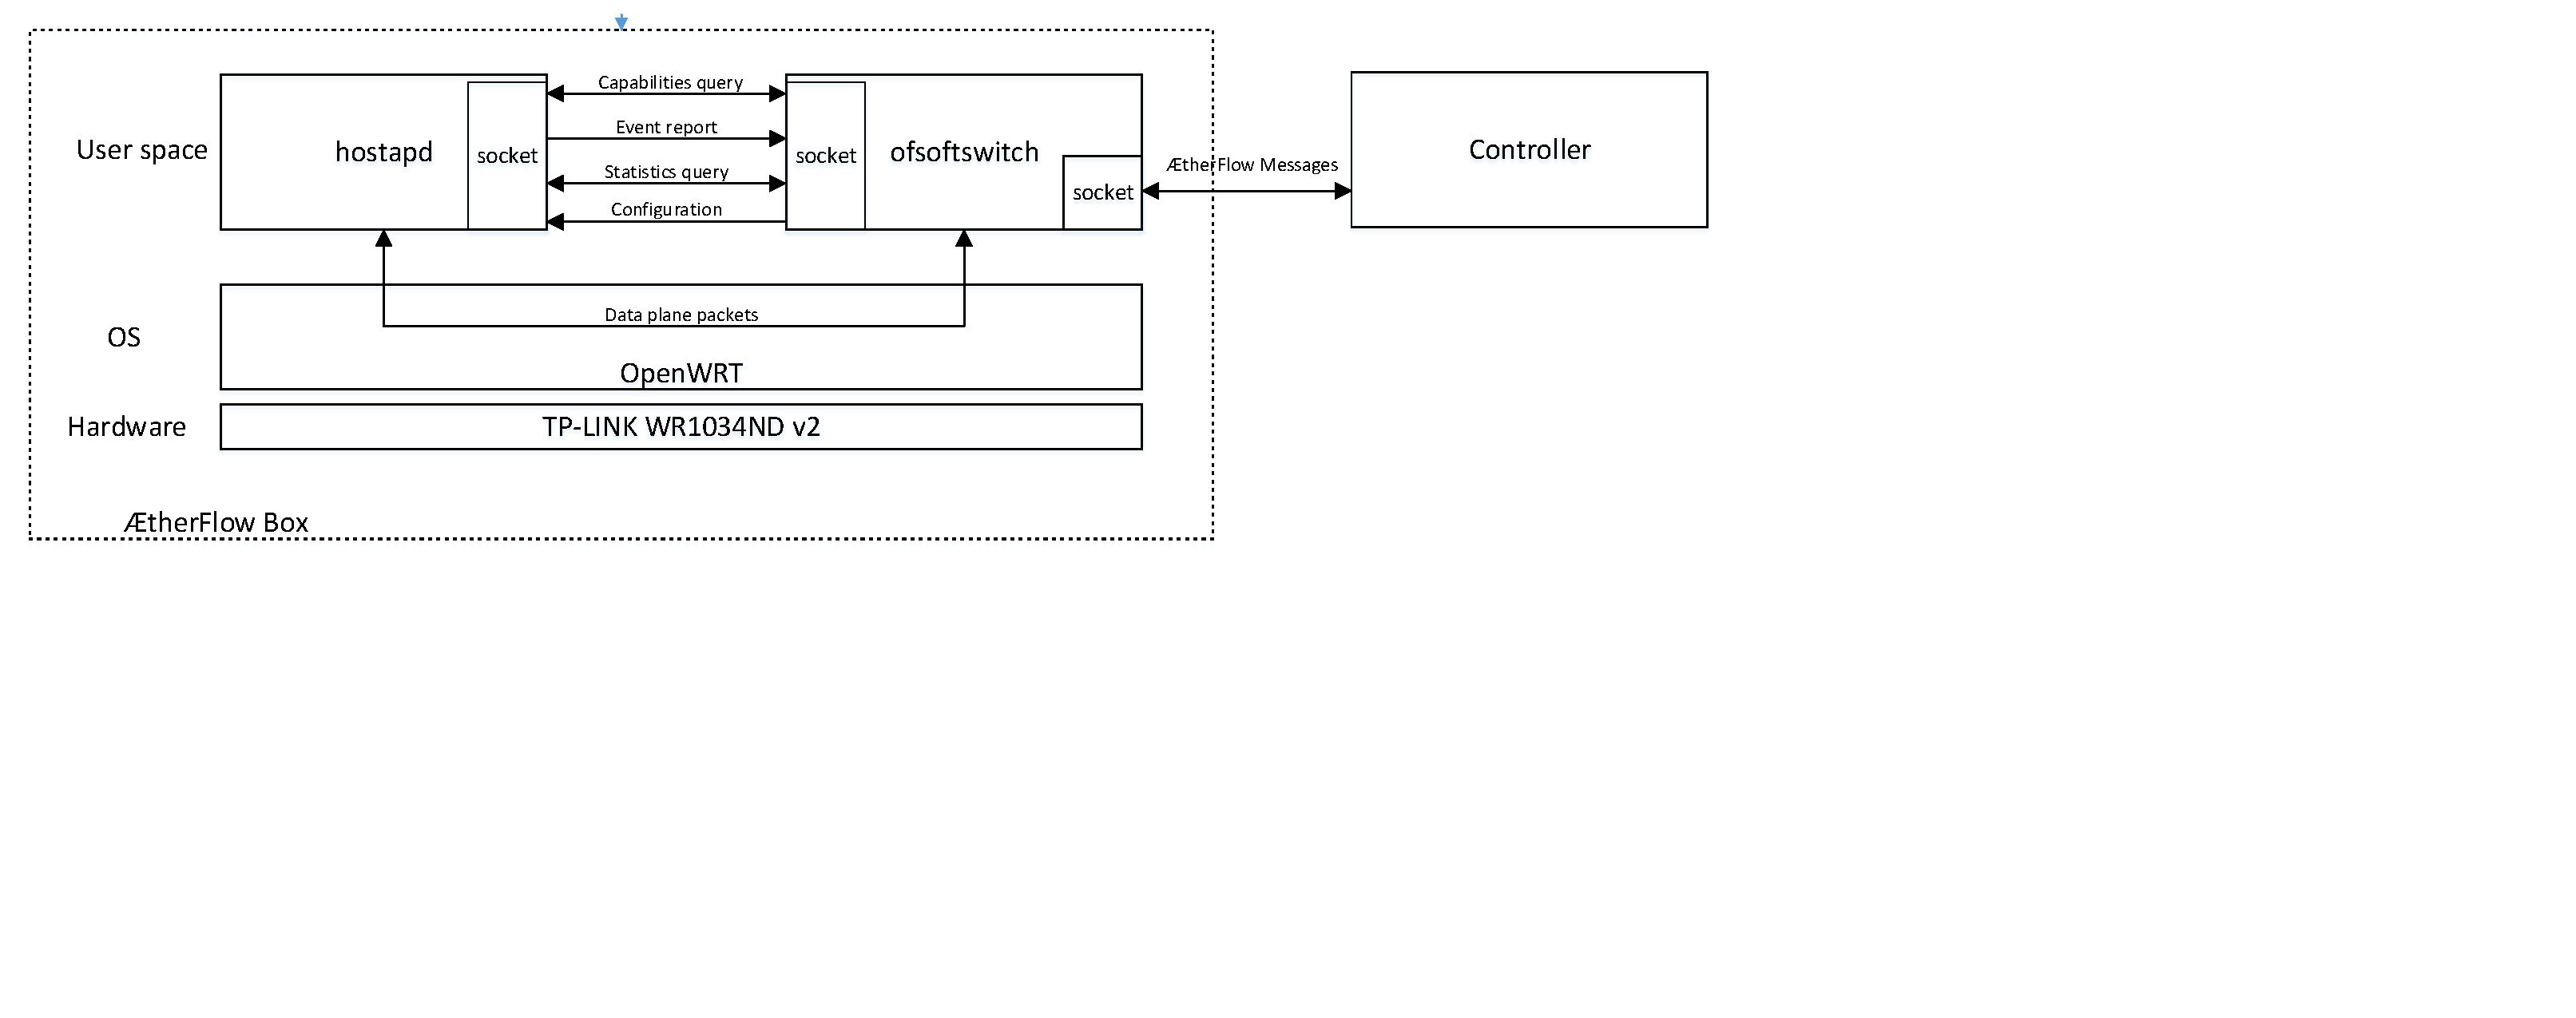
\includegraphics[trim=.2in 3.75in 7in .2in, clip, width=1.0\textwidth]{figures/implementation}
\caption{Implementation of \aetherflow.}
\label{fig:impl}
\end{figure*}

To validate our design and to demonstrate the viability of the \aetherflow
framework as a platform for the development and deployment of intelligent
wireless SDN applications, we implemented and deployed \aetherflow on a commercially
available access point. 

We chose the access point TP-LINK WR1034ND v2 as the hardware 
platform for our implementation.  This AP has five 100Mbps Ethernet ports and one
3-antenna radio interface, supporting protocols IEEE~802.11b/g/n.  We replaced
the firmware of the AP with OpenWRT 14.07 Barrier Breaker. OpenWRT
is an open source Linux distribution designed for network embedded systems.
Network utilities are integrated in OpenWRT and are optimized in size to fit in
embedded environments which usually do not have as much resources as general
purpose computer systems. In OpenWRT, when the radio interface is set up as an
access point, its data plane is managed by Linux kernel and its control plane
is run in the user space by daemon \texttt{hostapd}. 

The native OpenWRT system does not support SDN. To make our access point an SDN
switch, we used the open source CPqD SoftSwitch (\texttt{ofsoftswitch}), which implements an OpenFlow v1.3 pipeline and switch
agent that can be deployed on OpenWRT system.

An \aetherflow data plane extension is then implemented in
\texttt{ofsoftswitch}. The extension adds in wireless physical and logical
ports that are mapped to the radio interface and access points managed by \texttt{hostapd}. To
establish communication between \texttt{ofsoftswitch} and \texttt{hostapd},
\texttt{hostapd} is also modified to enable control of AP from
\texttt{ofsoftswitch} and event reporting from AP to \texttt{ofsoftswitch}. The two
processes communicate via a Unix socket in the OpenWRT system.  An overview of this
implementation is depicted in Figure~\ref{fig:impl}.

Whenever an event related to a mobile station is triggered in \texttt{hostapd},
the event summary is sent to \texttt{ofsoftswitch}, which forwards it to
the controller using the event port message. Whenever a statistics request from the
controller is received by \texttt{ofsoftswitch}, the request is forwarded to
\texttt{hostapd}, and the statistics data is sent to \texttt{ofsoftswitch} and
then sent to the controller with a statistics reply message. Similar behavior
occurs for capability queries and configuration updates.

\section{\aetherflow Applications}
\label{sec:application}
The design of \aetherflow extends the capability of OpenFlow to wireless
(specifically IEEE~802.11) interfaces in a natural way. \aetherflow enables applications to control both wireline switches and wireless access points. 
%First, it enables an
%SDN controller to gain a more comprehensive control over wireless APs and mobile
%stations. Second, \aetherflow enables an SDN controller to control at the same
%time wireline switches and wireless access points in the network. 
As a result,
network applications that used to require different protocols and cooperation of
software from different vendors can now be implemented easily using the
\aetherflow framework. 

We use a Layer~2 fast handoff application to demonstrate the flexibility and new functionality offered by the \aetherflow framework. 
% enables more powerful network applications to be developed on SDN systems.
This application
aims to facilitate the process of mobile station handoff within the same subnet
during which a device's Layer~3 address is not changed.

% Traditional Layer~2 switched network learns mobility of a mobile client when it
% receives a packet from the client on a different port. This process is not
% completed and can lasts for a significant amount of time if no packet is sent by
% the client after the handoff. During the handoff process, any packet going to
% the client will be lost. In SDN solutions such as OpenFlow, the controller
% learns client mobility by receiving a packet-in message. However, A packet-in
% message cannot be triggered until the client sends a packet after handoff,
% resulting in the same problem as Layer~2 switched network.

% A Layer~2 fast handoff application is made possible by \aetherflow since it
% provides the SDN controller with wireless interface information, such as probe,
% association, client's signal strength, etc. With these information, when handoff
% occurs or even before that, the SDN controller may actively reconfigure
% switches in the network so that packets going to the client are redirected to
% the new AP that the client is associated to.

A typical Layer~2 fast handoff application runs in three phases. The
first phase is handoff prediction. The controller collects signal
strength information of the mobile stations by requesting statistics
of all mobile stations associated with APs under its control. At the same
time, it receives the probe signal strength of the mobile stations measured by
other APs from the probe event reports. By keeping these data updated in a
timely fashion, the controller may predict that a handoff is about to happen, e.g.
when the mobile station's signal strength to its associated AP gradually weakens
while the signal strength to another AP gradually strengthens. 

% A more accurate prediction is
% possible if history data and appropriate prediction model is used.

The second phase of the Layer~2 fast handoff application is multicasting. When a
handoff prediction of a mobile client is made, the controller multicasts all the
packets with the client as destination to both its current associated AP and the
predicted AP. The action is completed by
modifying the flow entries of the switches in the network. Multicast guarantees
that the client can receive packet immediately after it reassociates with the
new AP, thus minimizing the packet loss during the handoff.

The third phase is flow redirection. After the multicasting phase, if the client
associates with a new AP, the multicast is stopped and all the following packets
to the client will be redirected to the new AP. If the prediction is wrong and a
handoff did not occur within a certain timeout period, multicast is stopped and
all the following packets will be forwarded to the original AP that the client
is associated to. \aetherflow makes the decision possible with event report
interface that provides client association event report to the controller.

Other than Layer~2 handoff application, wireless network applications such as
client steering, user-based QoS control, etc.\ can also be easily implemented
using \aetherflow framework.

\chapter{\uppercase {\crossflowcap Implementation}}
\label{sec:evaluation}

\section{Illustrative \crossflow Implementation}

In this section, we describe our implementation of \emph{adaptive modulation}, \emph{frequency hopping} and \emph{cognitive radio} applications using the \crossflow framework. For illustration, we implement our model on a USRP N210 embedded SDR from Ettus Research. The N210 provides a Zynq 7020 All Programmable SoC, which combines a dual ARM Cortex-A9 processor and FPGA on the same device. We use the CPqD Softswitch~\cite{ofsoftswitch13} (\texttt{ofsoftswitch}) software as the switch agent in the SDN model. Its main functionality is to enable communication between GNU Radio and the python based Ryu SDN controller. As described in previous sections, the applications will send messages to the processing blocks, e.g., to configure them. The \texttt{ofsoftswitch} then forwards this request to a centralized \texttt{\crossflow Hub} inside the GNU Radio domain. 

%The responsibility of this block is to switch the request according to the specified processing block. In our current model shown in Figure~\ref{fig:message_block}, we implement the interface requirements for two blocks: Modulators and Sink. The \texttt{Mod Controller} and \texttt{USRP Controller} blocks are responsible for translating the request messages into implementable actions for the processing blocks and also reporting the responses from the blocks to \texttt{CrossFlow Hub} for certain events supported by the blocks. In the current version, we are capable of providing configuration capability to the applications and we will soon incorporate event reporting and sensing capability into the implementation.
\begin{figure}[t]
  \centering
  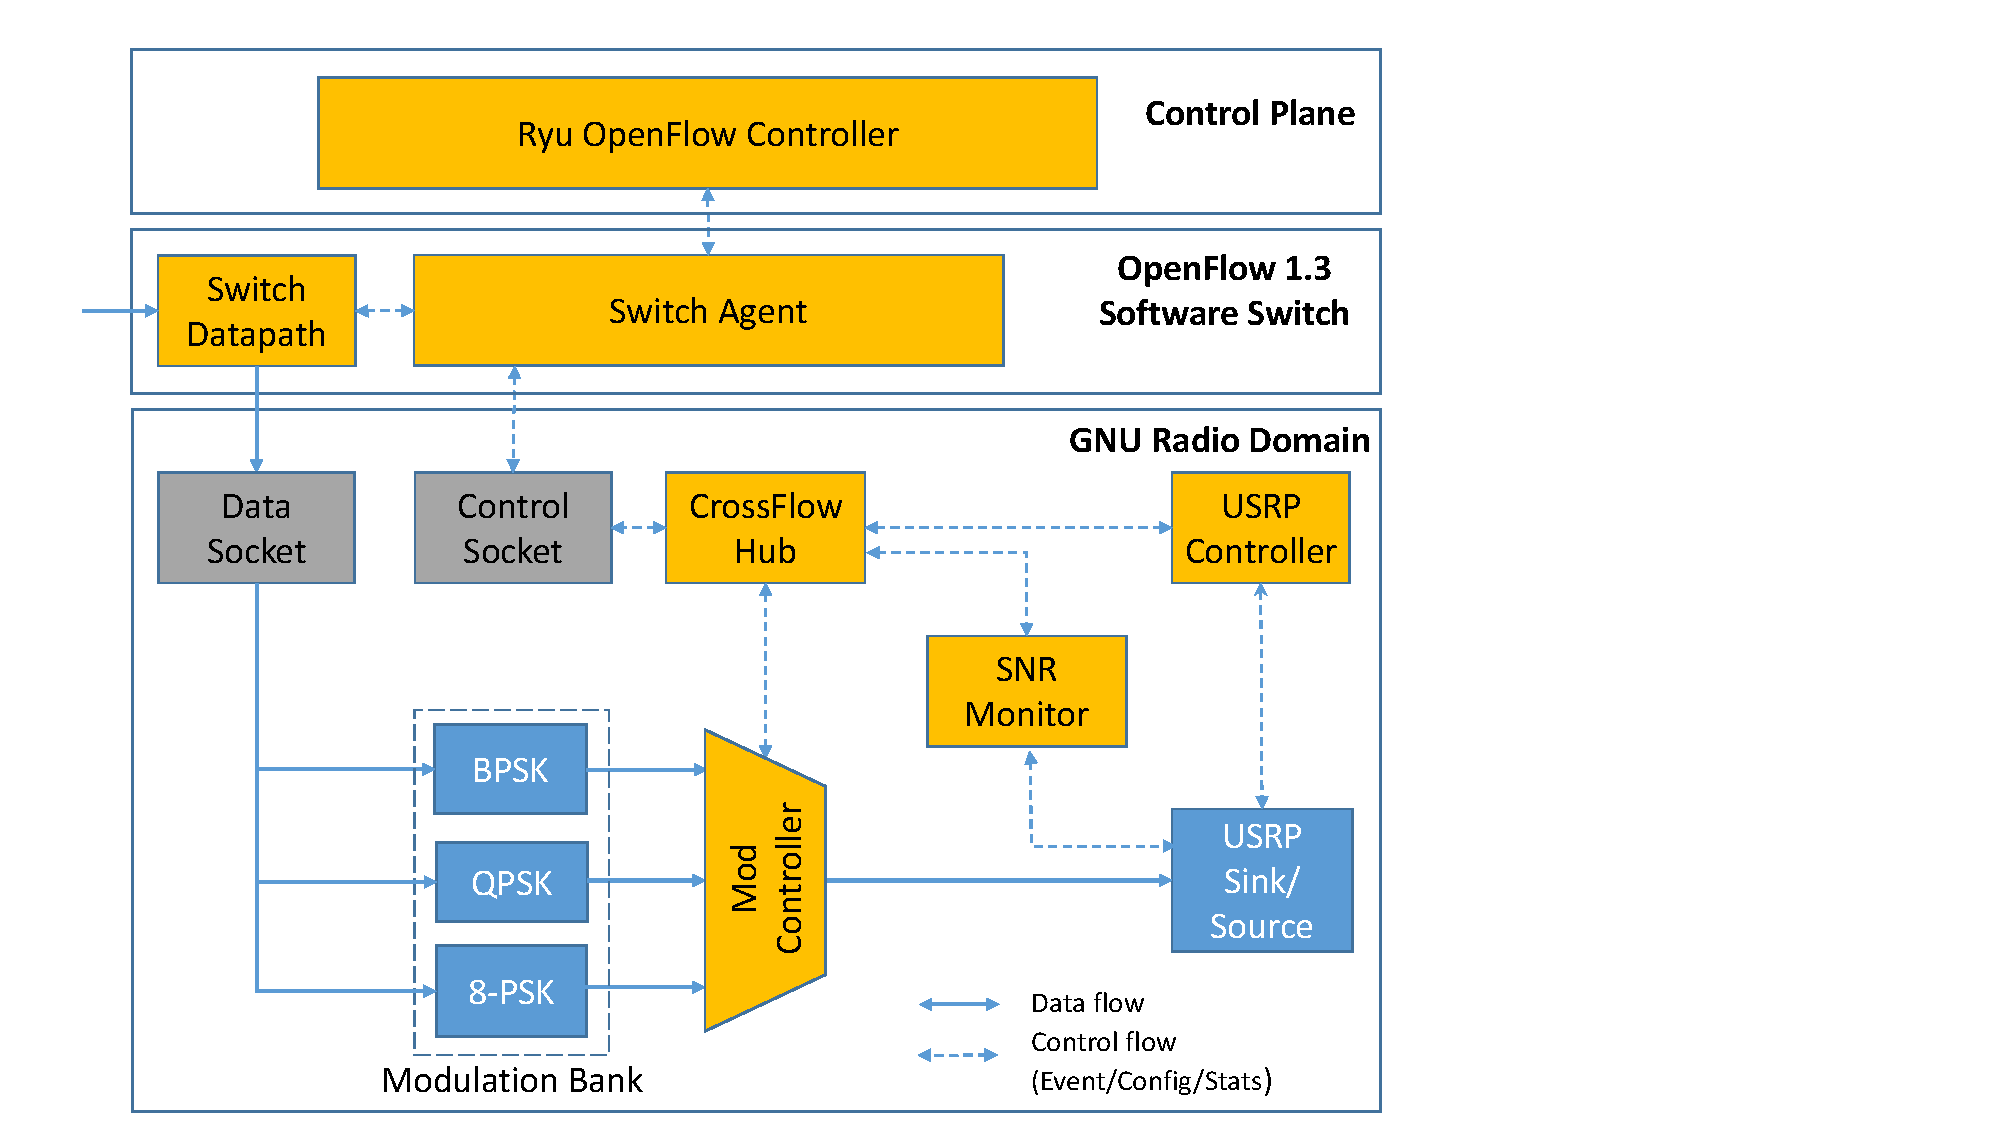
\includegraphics[width=0.8\textwidth]{figures/Flowgraph.pdf}
  \caption{Transmitter implementation diagram of \crossflow with two processing blocks: Sink and Modulators.}
  \label{fig:flowgraph}
\end{figure}

There are four main components (blocks) in the illustrative \crossflow module, as given in Figure~\ref{fig:flowgraph}, that we implement in GNU Radio, namely, the \texttt{\crossflow Hub}, the Modulation Controller (Mod Controller for brevity), and the USRP Controller.
\begin{itemize}
\item The \texttt{\crossflow Hub} is the interface between the Mod and USRP controllers in GNU Radio and the Ryu SDN controller. The \texttt{\crossflow Hub} and the Ryu SDN controller communicate via Socket PDU. The \texttt{\crossflow Hub} is responsible for receiving commands from \texttt{ofsoftswitch} (or any other compliant interface), interpreting the commands, and forwarding the commands to the appropriate controller block (i.e., either the USRP controller or Mod controller in our implementation). It is also responsible for receiving information from different controller blocks and sending information to the Ryu SDN controller. The \texttt{\crossflow Hub} has in/out ports to send commands and receive information to/from the GNU radio controller blocks. It also has in/out PDU ports for interfacing with Socket PDU.
\item The Mod Controller is one of the main controllers in the design. It is responsible for receiving commands from the \texttt{\crossflow Hub}, and selecting the appropriate modulation scheme from the modulation bank. For illustration, we include three modulation schemes in our modulation bank (BPSK, QPSK, and 8PSK); however, thanks to the modular design, we can easily add more schemes. The Mod Controller can also feedback information to the Ryu SDN controller about the modulation scheme that is currently in use and the number of modulation schemes available in the modulation bank.
\item The \texttt{SNR Monitor} is responsible for monitoring the SNR level and generating an event in case the SNR level falls below a certain threshold, which can be configured by the application. Currently the framework uses the existing SNR probe of GNU Radio, which supports four $M$-PSK SNR estimators. This monitoring block is also responsible for relaying the SNR statistics back to \texttt{\crossflow Hub} in response to a SNR statistics query generated by the application.
\item The USRP Controller is another controller block in the \crossflow module. It is responsible for controlling different RF parameters of the USRP Transmitter/Receiver based on commands from the \texttt{\crossflow Hub}. In our proof-of-concept implementation, we control the carrier frequency and the power of the signal. It can also feedback information to the \texttt{\crossflow Hub} about the current RSSI, temperature, SNR, carrier frequency, power, etc.
\end{itemize}
Although our illustrative implementation only has two controllers (one facilitating abstraction of the USRP Sink/RF implementation and the other facilitating abstraction of the adaptive modulation implementation), additional controllers can be easily added to support new applications, functionalities, and abstractions.
%As we mentioned before, for this implementation, we have two controllers, but its design is modular, and more controllers can be added easily to support new applications/functionality.

\section{Example Applications}


\subsection{Frequency Hopping Application}
Frequency hopping is a technique of transmitting radio signals by spreading the signal over a sequence of changing frequencies. It has tremendous application in military as it is used against jamming and for protecting against unauthorized eavesdropping. For implementation, the receiver of the signal must be aware of the sequence of frequencies so that it can tune into the appropriate channel. This requires synchronization between the transmitter and the receiver. In \crossflow, we implement this application easily as only the controller needs to be aware about the predetermined sequence. This sequence can even be dynamic according to the channel conditions and policies.   

\subsection{Adaptive Modulation Application}
Adpative Modulation is a technique where the modulation is changed according to the conditions of the channel. There are various estimators which are used for obtaining channel quality. These can be Signal-to-noise ratio (SNR), Bit error rate (BER) and other environment specific estimators. For illustration, we assume a fixed sequence for changing the modulation schemes every 5 seconds. 

\subsection{Cognitive Radio Application}
We build upon the frequency hopping application mentioned above to construct a cognitive radio application. Cognitive radio is a type of radio in which the device is aware of its environment and can dynamically change its operating parameters like transmission power, frequency, gain etc in response to changing environmental conditions. In \crossflow, we implement an application that can configure a radio device to switch channels based upon a low SNR event measured by the device.

\chapter{\uppercase {Validation}}
\label{sec:validations}

\section{\aetherflow Validation}


We use the \aetherflow implementation described in \ref{sec:impl} to
evaluate the performance and demonstrate the viability of the \aetherflow
approach. 
Our results demonstrate that \aetherflow framework allows SDN 
applications to efficiently and dynamically configure wireless
networks without loss of performance. 

%In particular, we extend its
%capability by adding event report and statistics methods. We add a socket on
%both hostapd and ofsoftswitch13 sides for their inter process communication.
%When an event occurs, hostapd sends a notification to ofsoftswitch13 daemon to
%notify, and the daemon will then send to the controller with the corresponding
%experimenter message we defined above to notify the controller, if the event is
%of interest to the controller. When the controller needs to query the statistics
%of mobile stations on an access point, it sends the query to ofsoftswitch13
%first. ofsoftswitch13 forwards the request to hostapd. hostapd invokes API of
%driver to obtain the statistics and sends back the statistics to ofsoftswitch13,
%which then proxy the information back to controller.

%Supports of \aetherflow configurations also needs to be added. Authentication
%procedure of hostapd needs to be modified to support the authentication
%profile/group model. In particular, the original hostapd only supports `one-
%shot' authentication, i.e. only authenticate each mobile station once during
%the association procedure. Our model requires multiple attempts of
%authentication based on different profiles. The other configurations, including
%radio interface configuration and access point configurations, are implemented
%in a different way. Parameters in these configurations are all configurable
%with OpenWRT's UCI system. Therefore when such configuration requests are sent
%by the controller, the switch will handle them by invoking corresponding
%OpenWRT APIs to reconfigure the parameters.

\subsection{Experiment Setup}
Our experiment uses a simple network topology, shown in Figure~\ref{fig:topology}. 
It consists of two access points (AP1, AP2), a Layer 2 switch, a wireline 
traffic generator and a wireless 802.11 mobile station (STA).  We use an OpenFlow enabled
Layer 2 switch and  \aetherflow enabled APs as described in Section~\ref{sec:impl}. The mobile station has a single WiFi radio
interface. 

\begin{figure}
\centering
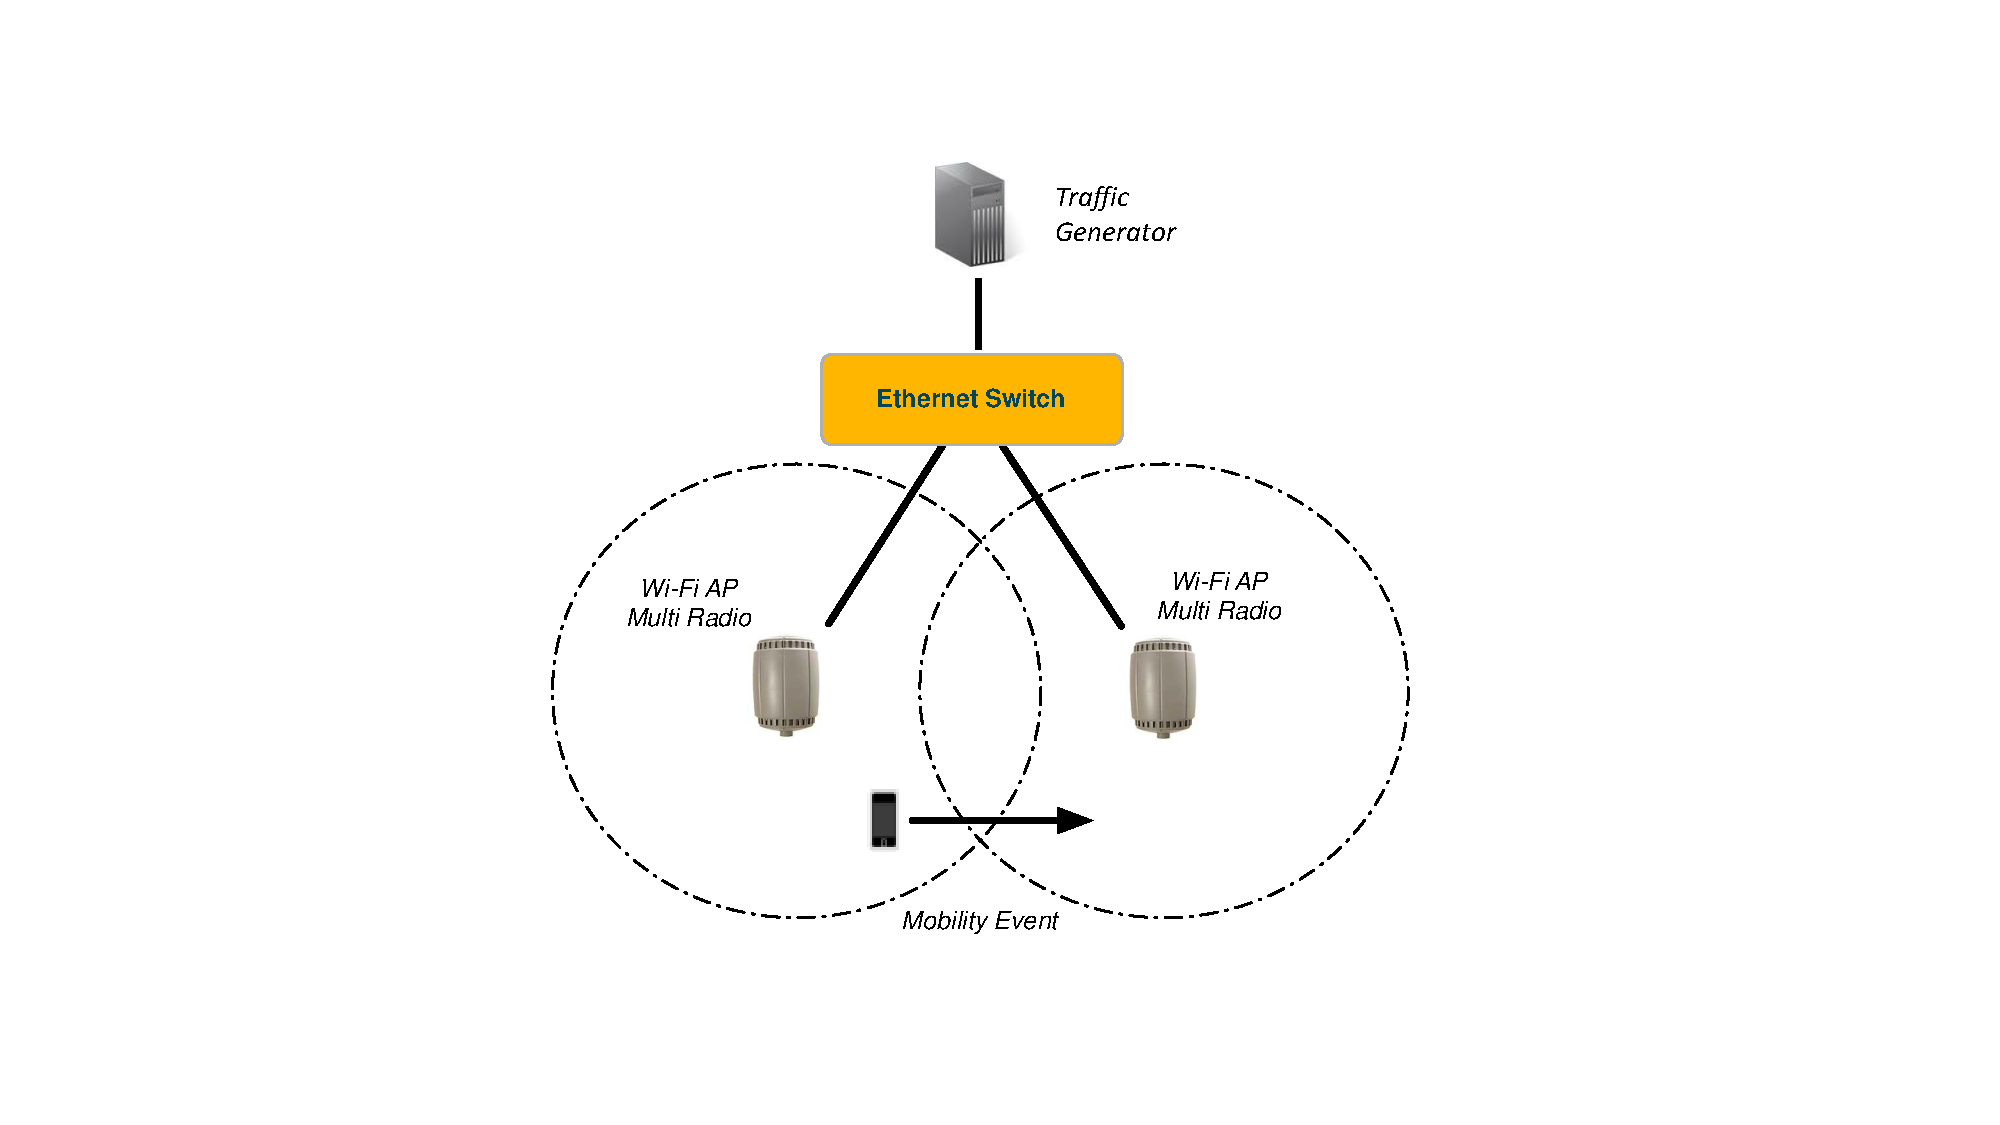
\includegraphics[width=1.0\textwidth]{figures/topology}
\caption[\aetherflow experiment network topology]{Experiment network topology\protect\footnotemark.}
\label{fig:topology}
\end{figure}

In our experiment, both APs and the traffic generator are connected to the switch
through  Ethernet. All the three boxes are connected to an OpenFlow
controller through a separate control plane subnet that is not displayed in the
figure.  The two APs are located at a certain distance and have overlapping coverage areas.  Both APs are configured with
the same SSID and use open authentication. 

\subsection{Layer 2 Handoff Application}
Our Layer 2 handoff application accords with what we described in
Section~\ref{sec:application}. The investigation of good
predictors and predictive models for handoff is beyond the scope of this paper.
In our implementation, the controller application always predicts that the
handoff of STA from AP1 to AP2 will occur seven seconds after the experiment starts.
The time period is selected solely for the purpose of this experiment and
does not apply for general cases. 
 
\footnotetext{Courtesy: flowgrammable.org}
After seven seconds, the controller starts to multicast packets going to STA to both
AP1 and AP2 by sending FlowMod messages to both APs and the switch. After STA
associates with AP2, the controller configures the switch to stop multicasting
and forward packets to only AP2. If the predicted handoff did not happen 15
seconds after the prediction, the controller reverts the multicast and forwards
packets to only AP1.



\subsection{Experiment Procedure and Results}
In each round of experiment, the mobile station is initially associated with AP1. Both the traffic generator
and the mobile station are assigned static IP addresses within the same subnet. Before the experiment
starts, a UDP \texttt{iperf} session with bandwidth of 9Mbps is initiated from
the traffic generator to STA.  After experiment starts, STA moves from coverage
of AP1 to coverage of AP2, which forces the client to handoff from AP1 to AP2.
We move STA in a controlled manner such that the handoff happens at seven seconds
after the experiment starts. This time is selected such that the handoff happens
almost immediately after the controller application initiates multicasting.  Throughput
and packet loss rate during each round of test is measured by iperf with an
interval of 0.5s. In each round of experiment, one of the following
configurations is used:
\begin{itemize}
\item {\bf Bridge configuration} uses neither OpenFlow nor \aetherflow. Instead,
the Layer 2 switch and the two APs use the Linux built-in learning bridge to
forward packets. This is the traditional way of configuring a Layer 2 network
with two access points and one switch. 
\item {\bf \aetherflow configuration with prediction} enables \aetherflow on the APs and the
switch, and the handoff is managed by the Layer 2 handoff application (described
above) running on the \aetherflow controller using the Ryu controller framework.  
\item {\bf \aetherflow configuration without prediction} enables \aetherflow on the APs and the
switch, and the handoff is managed by a similar Layer 2 handoff application as given above without enabling prediction.  
\end{itemize}

%\begin{figure*}
%\centering
%  \begin{subfigure}[a]{\textwidth}
%        \centering
%      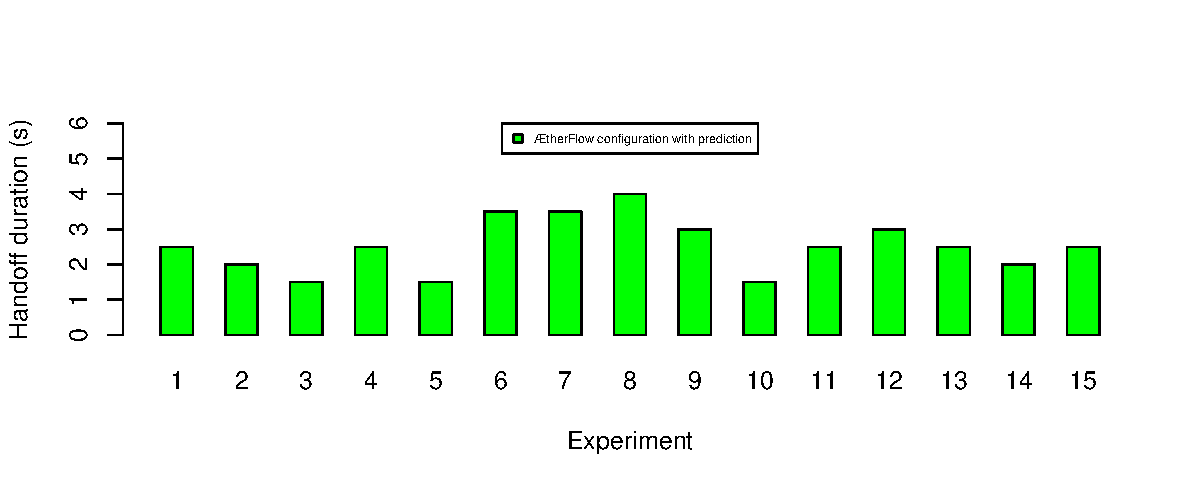
\includegraphics[width=1\textwidth]{figures/predduration.pdf}
%      \caption{Handoff duration for \aetherflow configuration with prediction}
%      \label{fig:pred}
%  \end{subfigure}

%  \begin{subfigure}[b]{\textwidth}
%        \centering
%      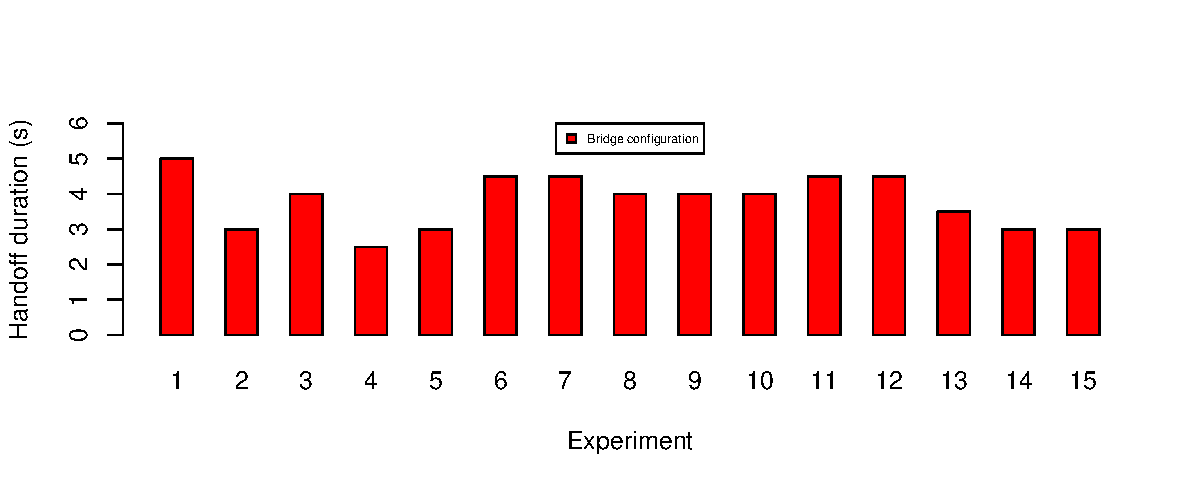
\includegraphics[width=1\textwidth]{figures/bridgeduration.pdf}
%      \caption{Handoff duration for bridge configuration}
%      \label{fig:bridge}
%  \end{subfigure}

%  \begin{subfigure}[c]{\textwidth}
%  \centering
%      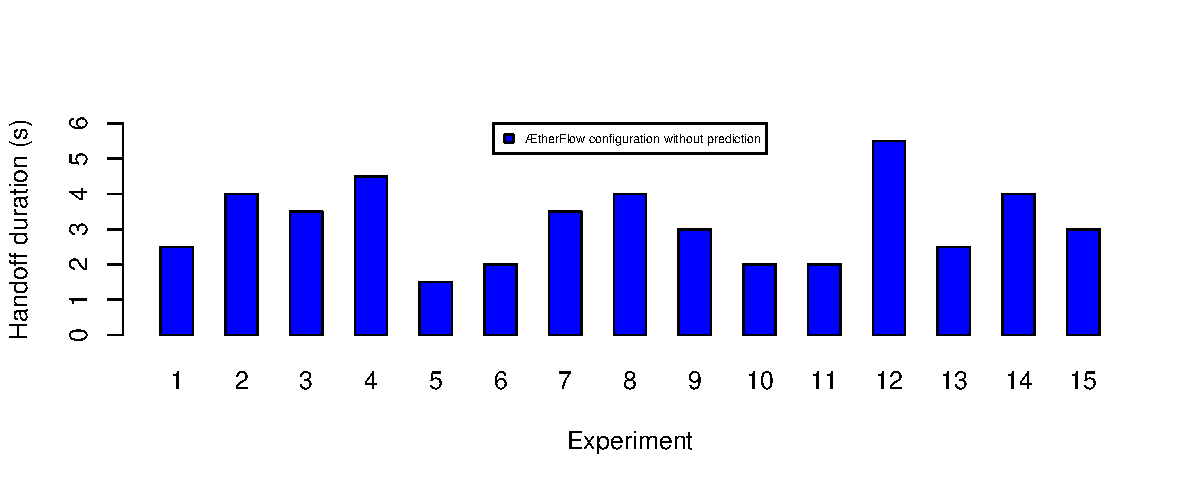
\includegraphics[width=1\textwidth]{figures/simpleduration.pdf}
%      \caption{Handoff duration for \aetherflow configuration without prediction}
%      \label{fig:simple}
%  \end{subfigure}%
%  \caption{Comparision of handoff duration for each experiment type}
%  \label{fig:duration}
%\end{figure*}

Fifteen rounds of experiments are conducted on each of the three configurations given
above. In a single round of experiment, the mobile station is considered to be
in handoff process during an interval after time $t$ = 7s if its average
throughput during the interval is less than 8 Mbps. By this criteria we can
determine the handoff duration of STA in each round of experiment. Our results, depicted  in Figure~\ref{fig:confidence}, indicate that the average handoff
duration of \aetherflow configuration with ~prediction across the fifteen rounds of experiments is
\textbf{2.53}s, which is lower than that of bridge configuration \textbf{3.8}s and \aetherflow configration without prediction \textbf{3.17}s.

We compare the traffic throughput and packet loss rate of the experiments
which have median handoff duration in \aetherflow with prediction and bridge configurations (experiment 3 for
bridge configuration and experiment 4 for \aetherflow configuration). 
The plots are shown in Figures~\ref{fig:throughput} and \ref{fig:loss}. 
These plots demonstrate that in terms of both throughput and loss rate, the \aetherflow
configuration recovers from handoff faster than the bridge configuration. 

\begin{figure}
\centering
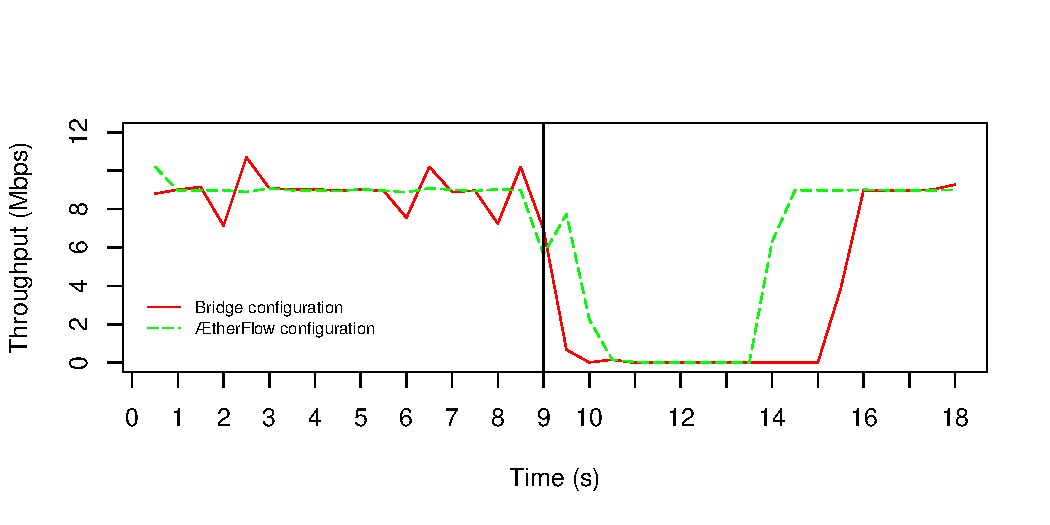
\includegraphics[width=.8\textwidth]{figures/throughput}
\caption{Comparison of throughput for \aetherflow with prediction and the baseline configuration.} % The throughput of
% \aetherflow configuration recovers from handoff in $5.5$ seconds, comparing to
% $7$ seconds in the bridge configuration.} % The total throughput of \aetherflow
% configuration during the handoff ($9$s to $16$s) is $24.5$M while that of the bridge
% configuration is $5.8$M.}
\label{fig:throughput}
\end{figure}

\begin{figure}
\centering
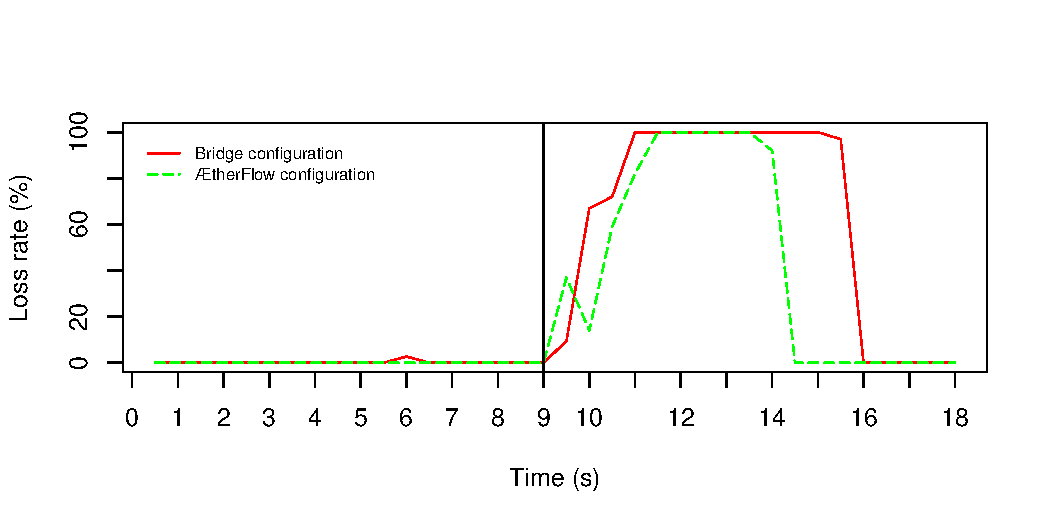
\includegraphics[width=.8\textwidth]{figures/loss}
\caption{Comparison of packet loss rate for \aetherflow with prediction and the baseline configuration.} % The packet loss
% of \aetherflow configuration recovers from handoff in $5.5$ seconds, comparing
% to $7$ seconds in the bridge configuration.}
\label{fig:loss}
\end{figure}

\begin{figure}
\centering
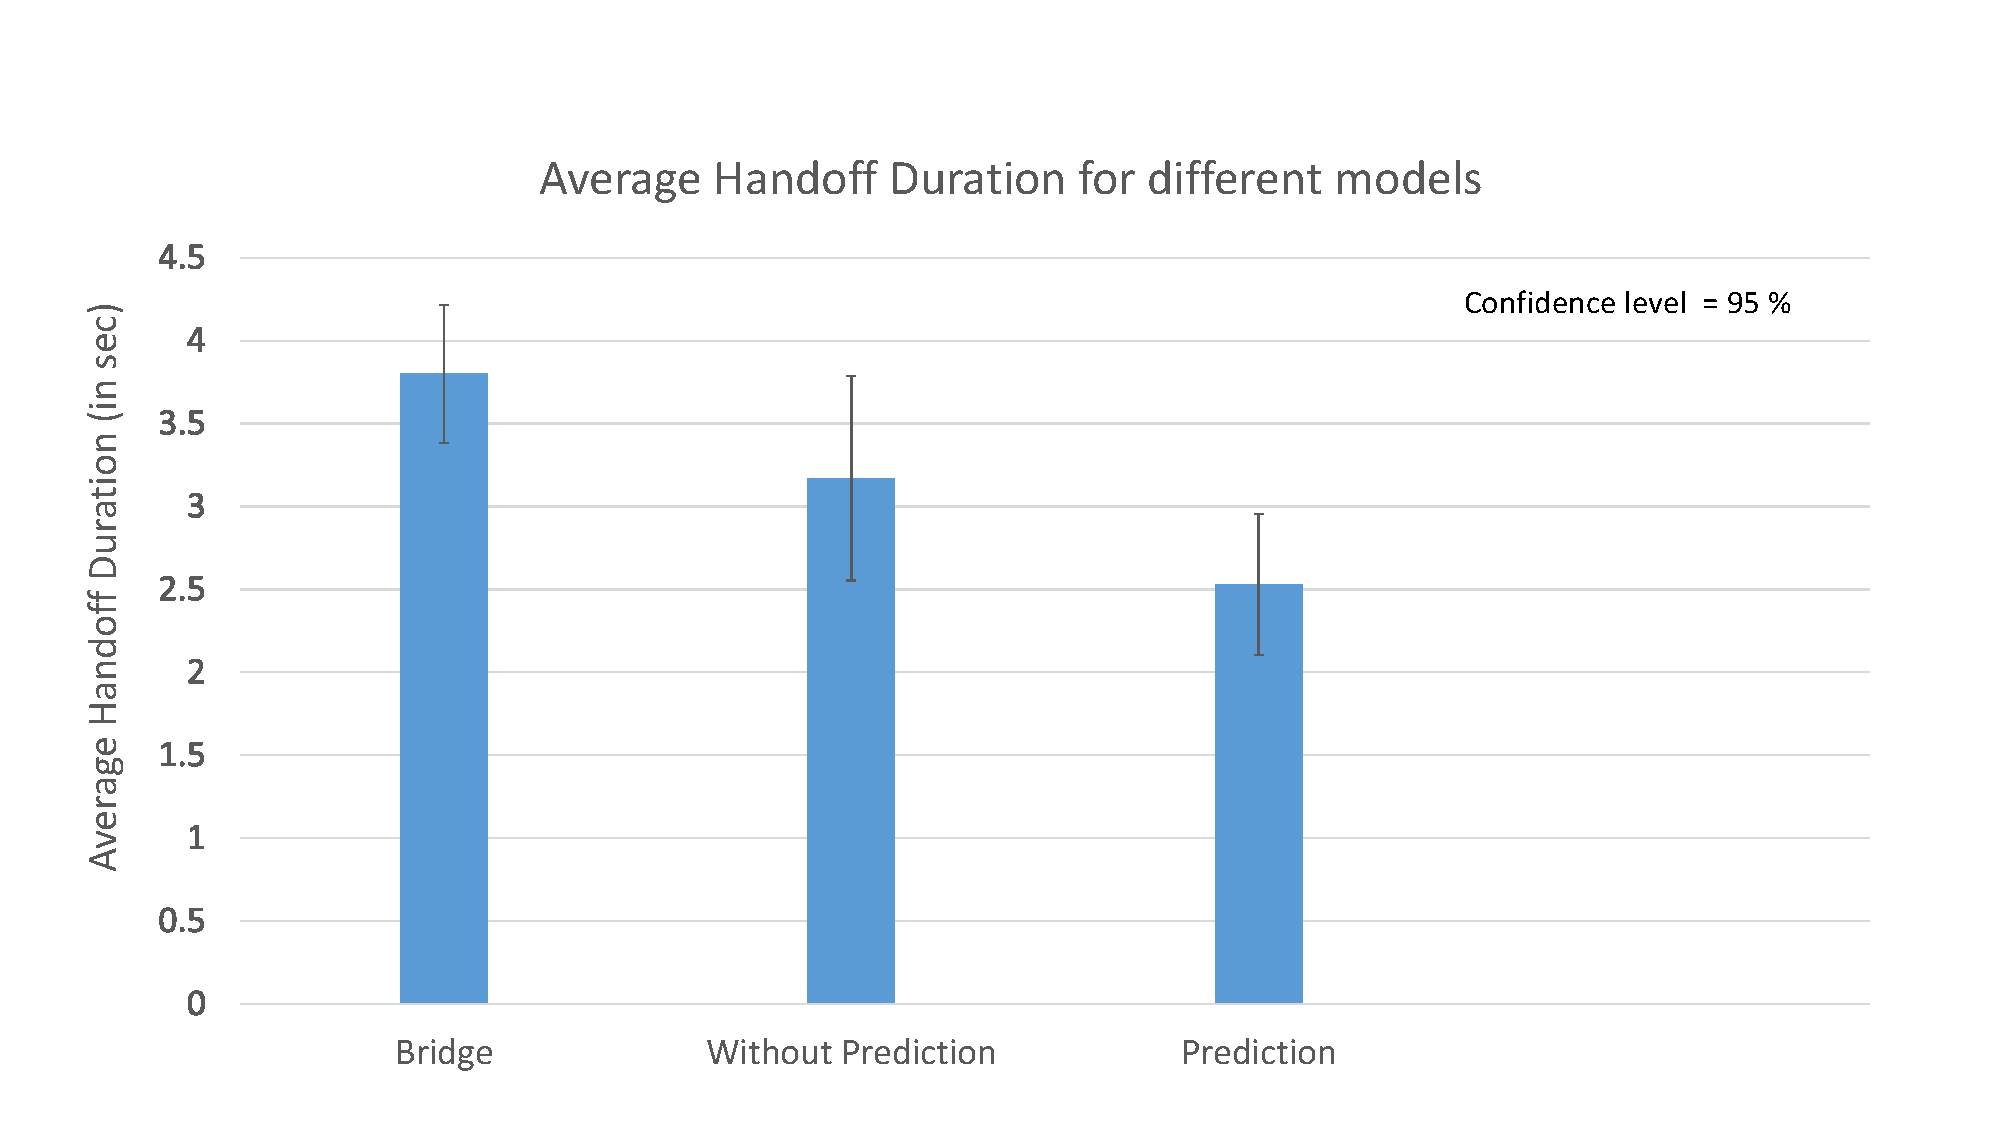
\includegraphics[width=.8\textwidth]{figures/confidence}
\caption{Comparison of average handoff duration for \aetherflow with different models and standard error.}
\label{fig:confidence}
\end{figure}

The experiment results show that even with the overhead induced by SDN data plane processing, the performance of Layer~2 handoff application based
on \aetherflow is better that of Linux kernel bridge configuration. % It shows
% that even with the overhead induced by SDN data plane processing, the
% performance of \aetherflow is comparable to that of the traditional configuration. % The results suffice
% for our proof-of-concept demonstration of the \aetherflow framework.



\section{\crossflow Validation}


We use the \crossflow implementation described in \ref{sec:evaluation} to provide a proof-of-concept validation of our design. We demonstrate the viability of \crossflow which  allows SDN applications to change the radio physical properties of wireless radio upon various qualifying parameters like channel conditions. 


\begin{figure*}
\centering
  \begin{subfigure}[b]{\textwidth}
        \centering
      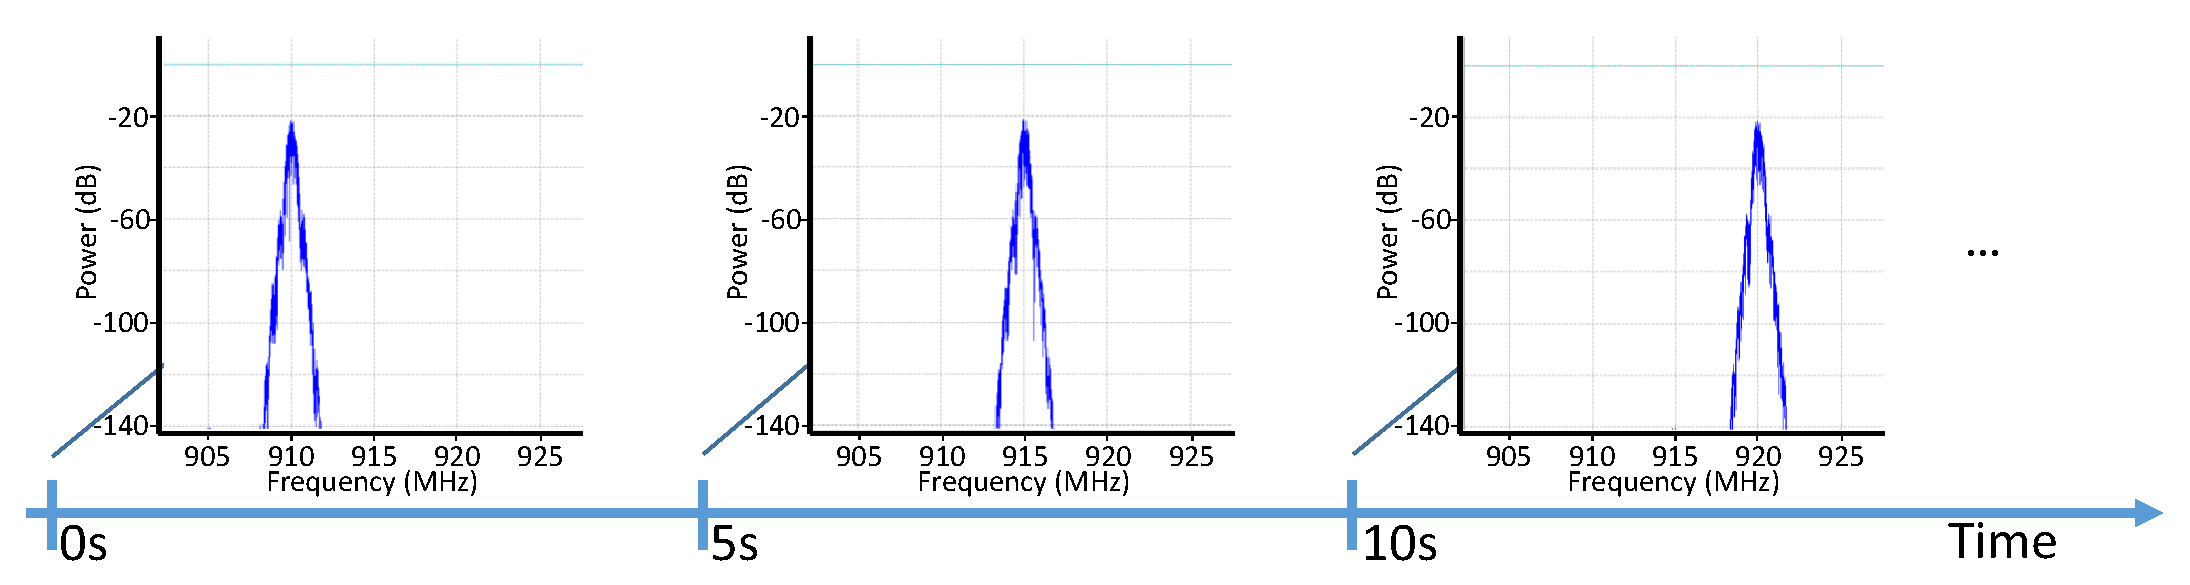
\includegraphics[width=1\textwidth]{figures/Freq.pdf}
      \caption{Spectral output for \emph{frequency hopping} application. The frequency changes every 5 seconds keeping BPSK as a fixed modulation scheme.}
      \label{fig:freq}
  \end{subfigure}

  \begin{subfigure}[a]{\textwidth}
  \centering
      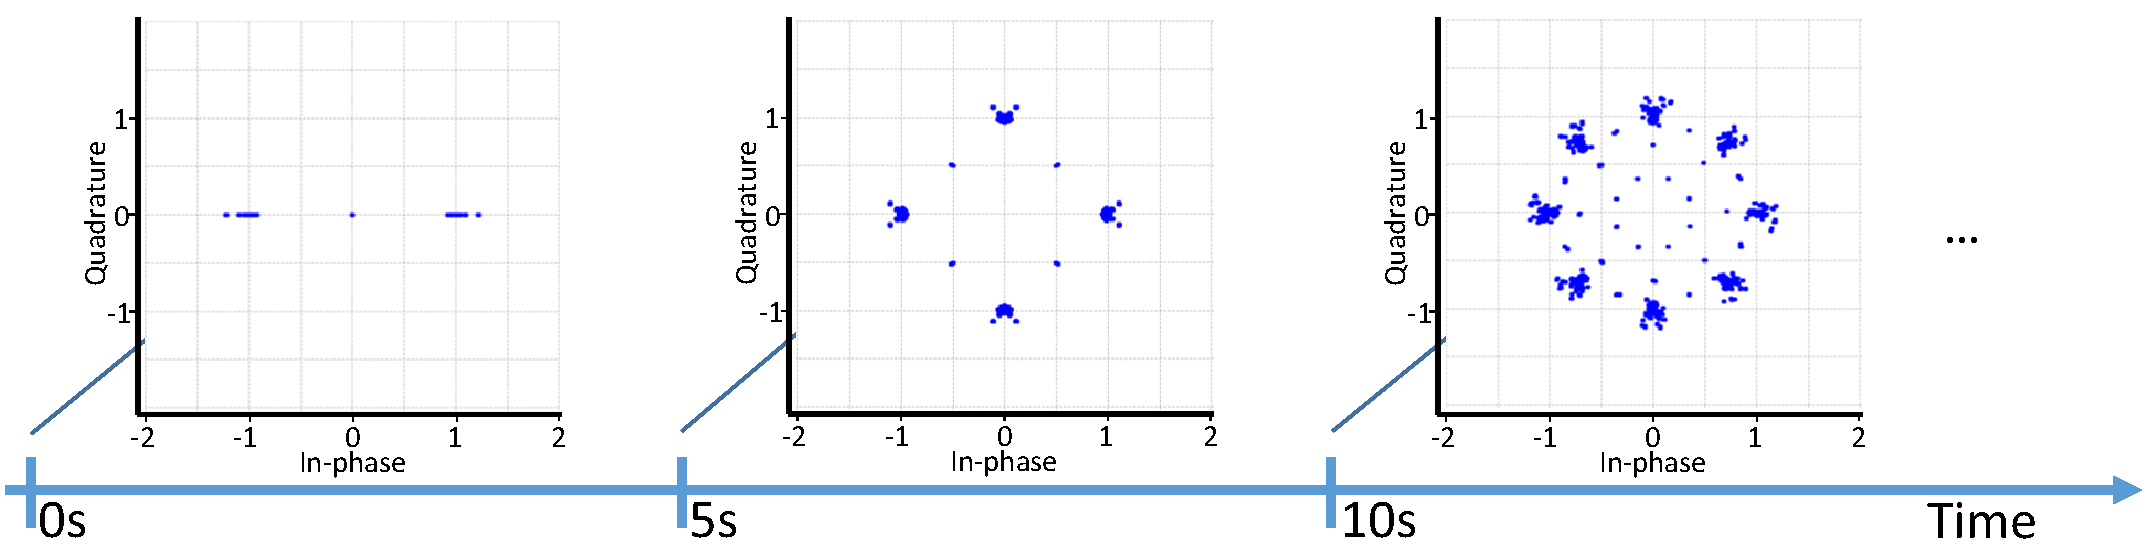
\includegraphics[width=1\textwidth]{figures/Mod.pdf}
      \caption{Constellation output for \emph{adaptive modulation} application. The modulation scheme changes every 5 seconds keeping a fixed frequency of 910 MHz.}
      \label{fig:mod}
  \end{subfigure}%
  \caption{Experimentation results for Frequency Hopping and Adaptive Modulation applications.}
\end{figure*}


\subsection{Frequency Hopping Application Implementation}

In this implementation,  the controller simply issues \emph{GNU-CONFIG-FREQ} command with desired frequency and pushes this configuration to the device. The \texttt{ofsoftswitch} receives this command and forwards it to the GNU Radio domain. The centralized \texttt{\crossflow Hub} inside the GNU Radio domain processes this request and issues appropriate commands to the  USRP Controller, which ultimately signals the USRP block to tune into the requested frequency. Figure~\ref{fig:freq} shows the experimental results where the sequence of changing frequencies is 910, 915 and 920 MHz and is changed every 5 seconds. For this application, we use a fixed BPSK modulation scheme.


\subsection{Adaptive Modulation  Application Implementation}

Similar to the \emph{frequency hopping} application, the controller issues the \emph{GNU-CONFIG-MOD} command with the appropriate modulation scheme (BPSK, QPSK, or 8PSK) and forwards the request to the device. The request ultimately reaches the Mod Controller, which is a multiplexer block that selects the requested modulation scheme. Figure~\ref{fig:mod} shows the results for changing the modulation scheme between BPSK, QPSK and 8PSK every 5 seconds, keeping a fixed carrier frequency of 910 MHz.

%\chapter{\uppercase {Architecture and Design}}
\label{sec:architecture}

In this section, we motivate and describe the overall architecture and design of \crossflow. In Section~\ref{sec:data_plane}, we introduce the proposed data plane abstractions. Then, in Section~\ref{sec:messages}, we describe how we extend the OpenFlow protocol to accommodate \crossflow messages.

%\begin{figure}[t]
%  \centering
%  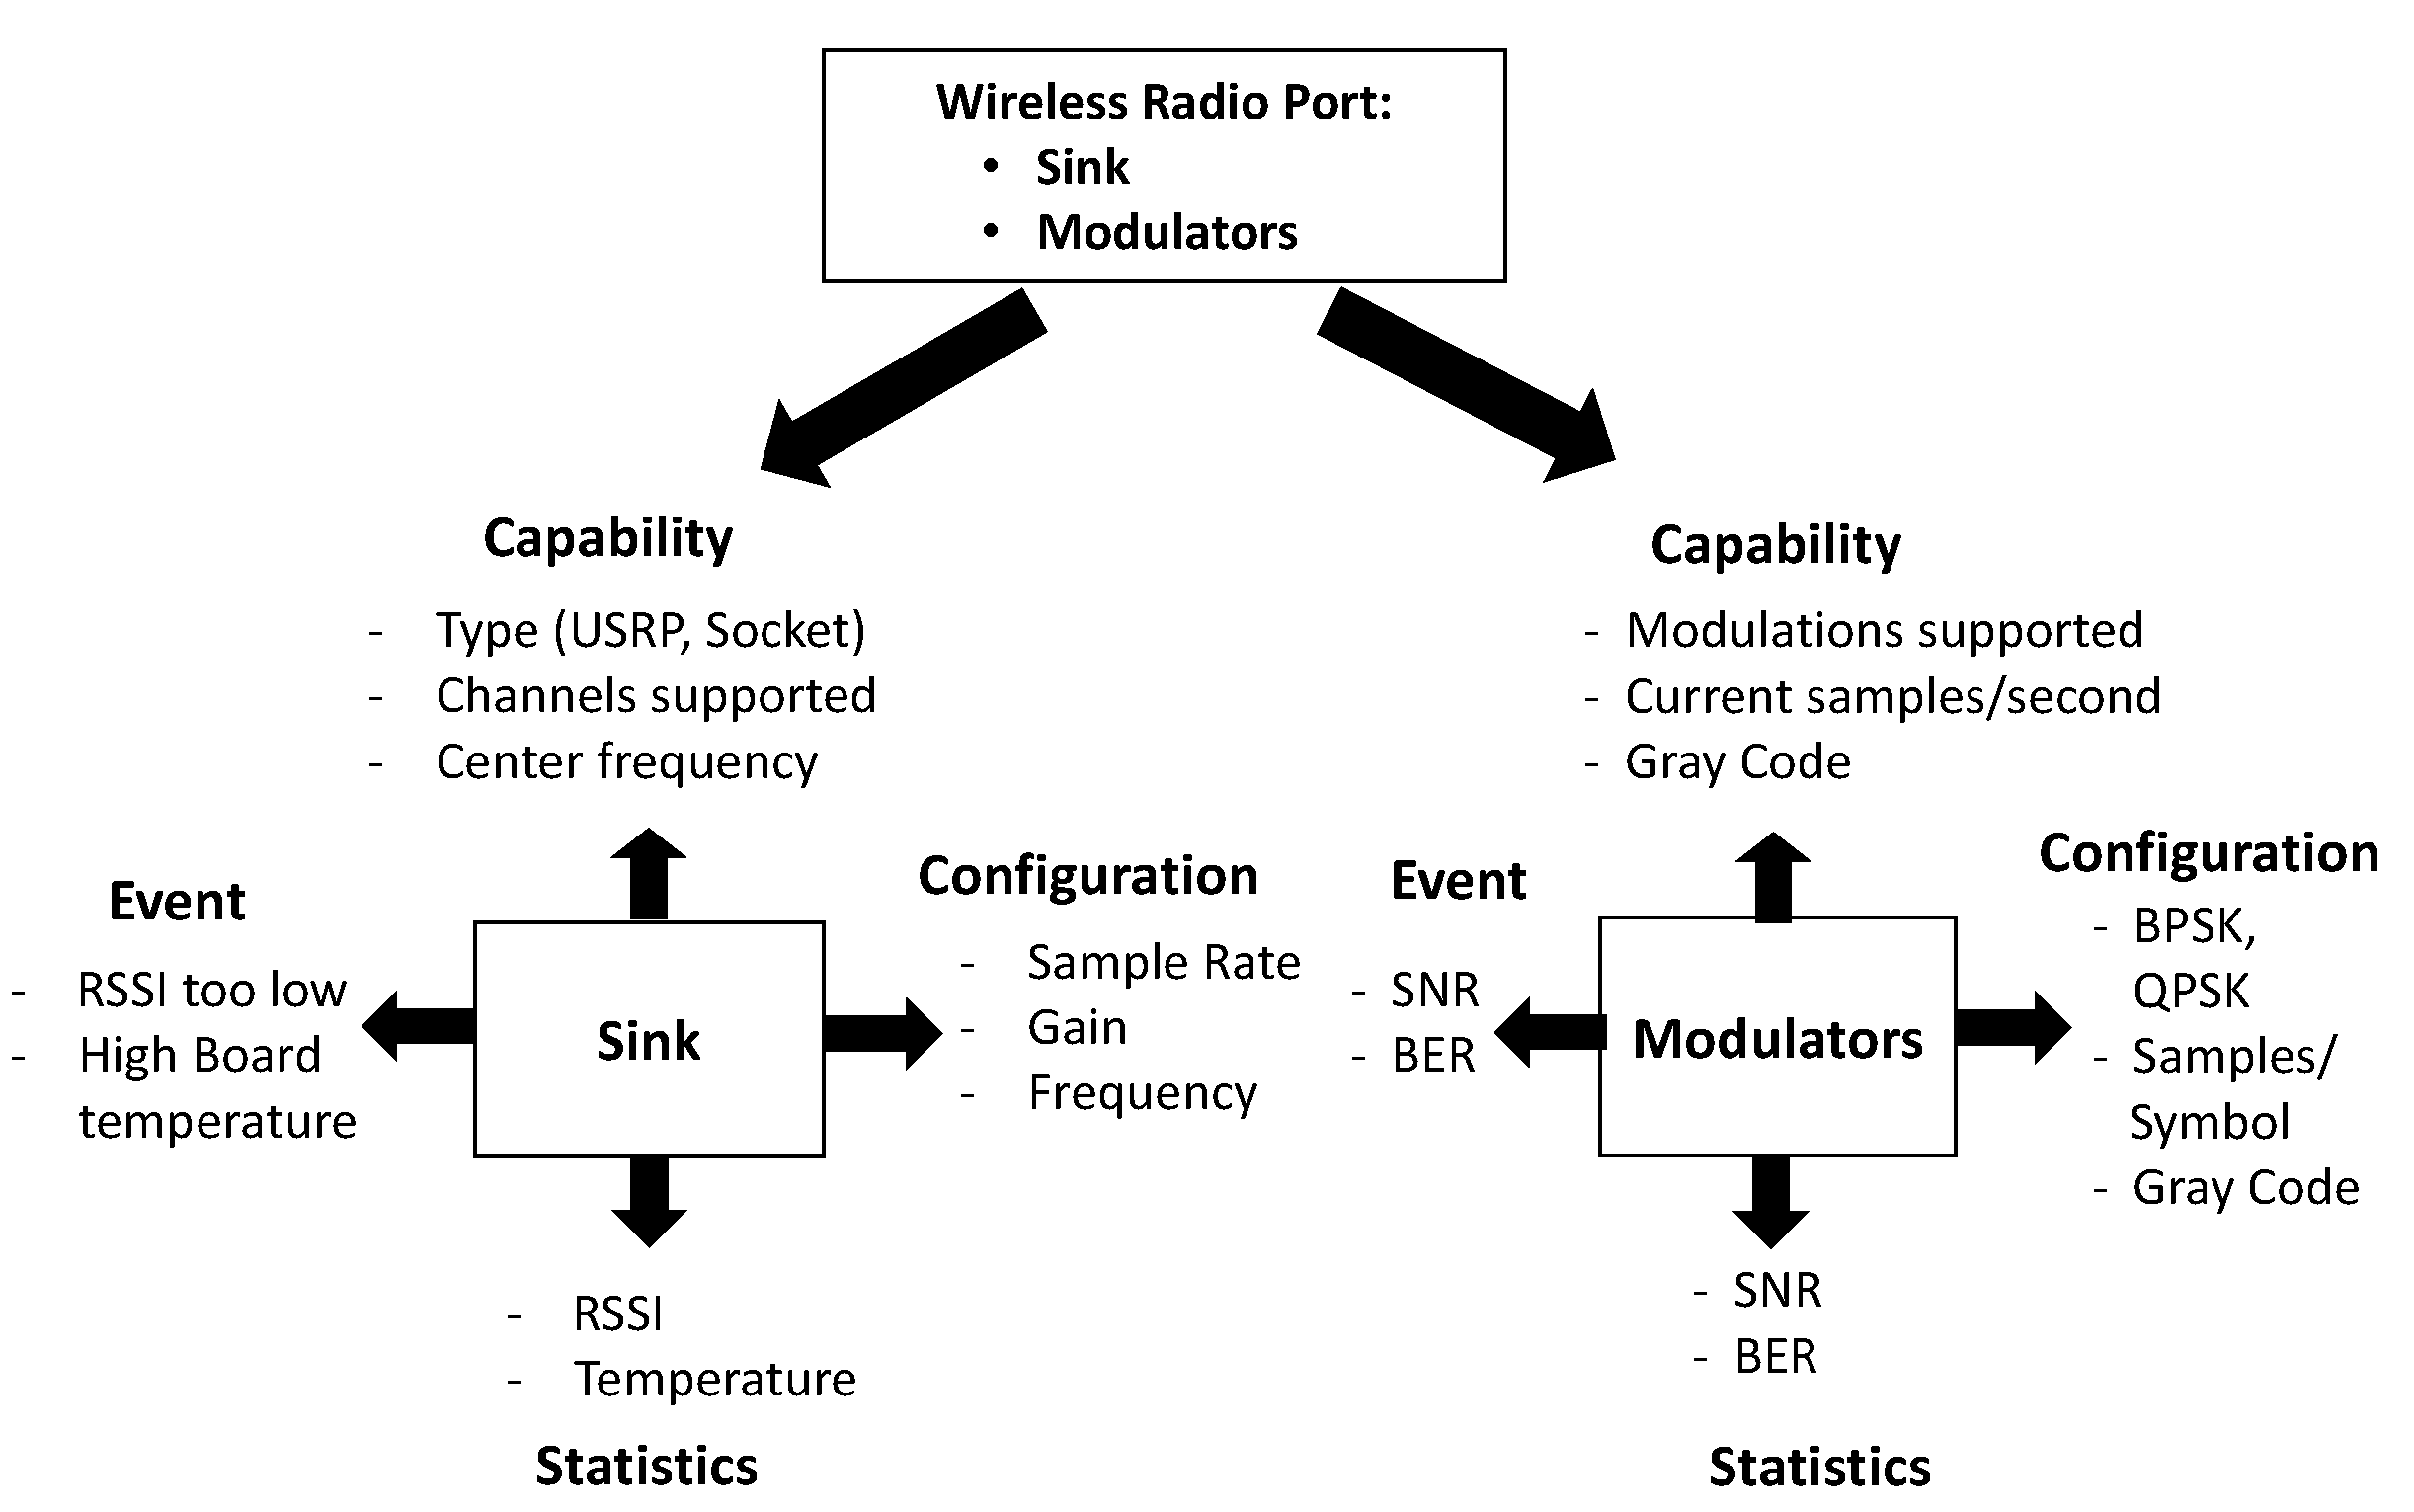
\includegraphics[width=0.48\textwidth]{figures/Interfaces.pdf}
%  \caption{Interface model for wireless radio port abstraction with two processing blocks: Sink and Modulators}
%  \label{fig:interface}
%\end{figure}

\begin{figure}[t]
  \centering
  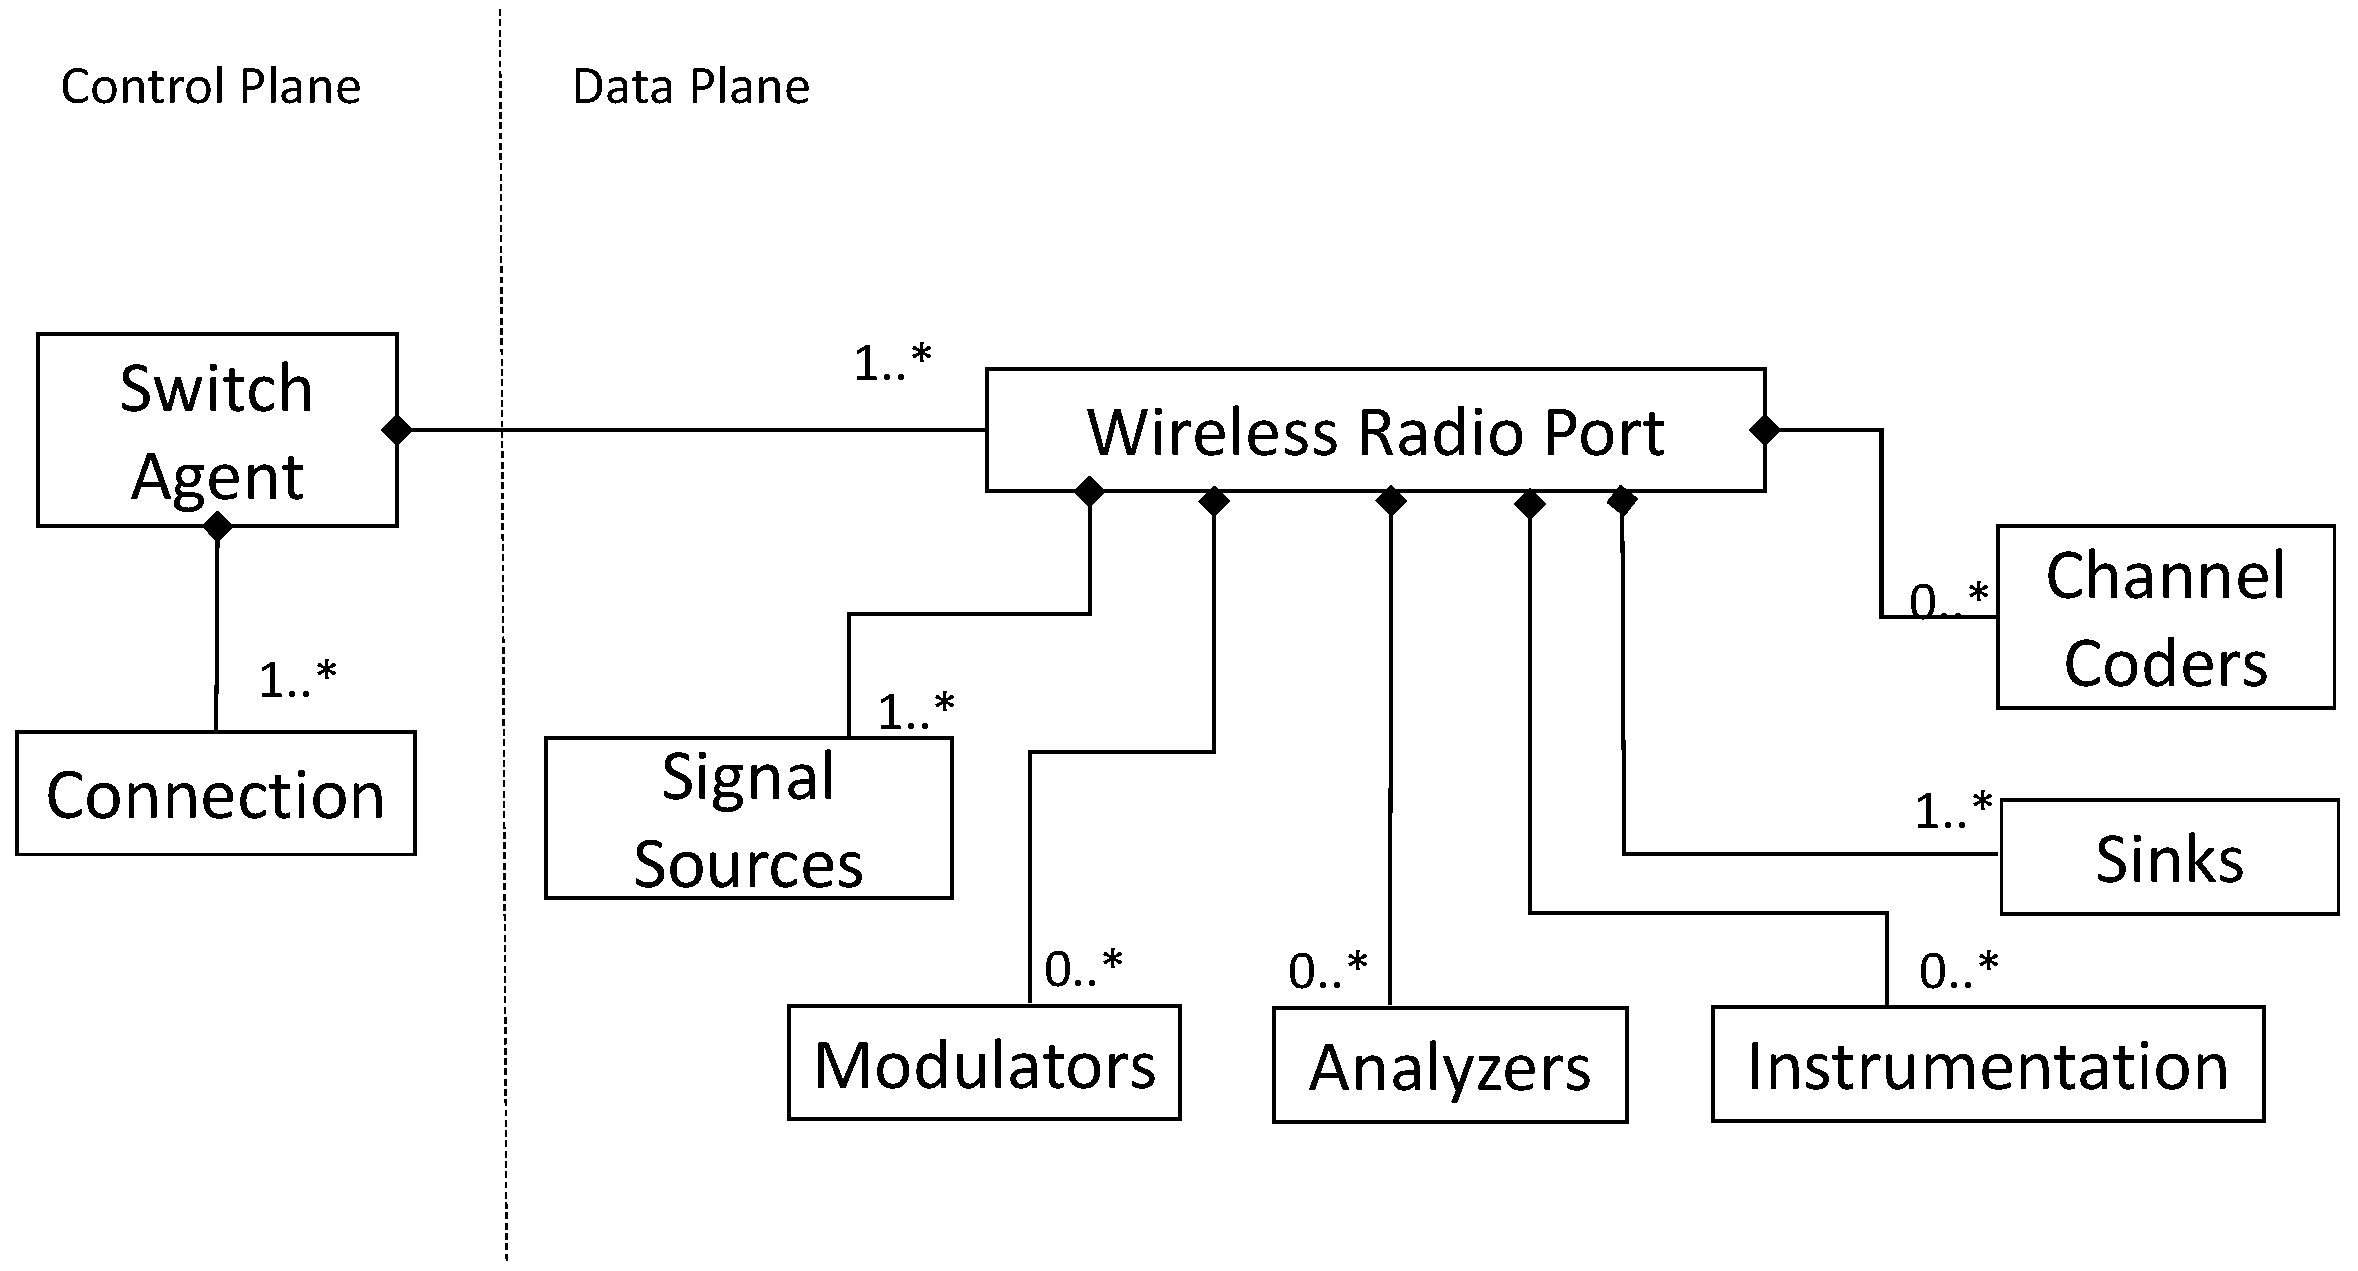
\includegraphics[width=1\textwidth]{figures/UML.pdf}
  \caption{Abstraction model of \crossflow}
  \label{fig:uml}
\end{figure}

%\begin{figure*}
%  \centering
%  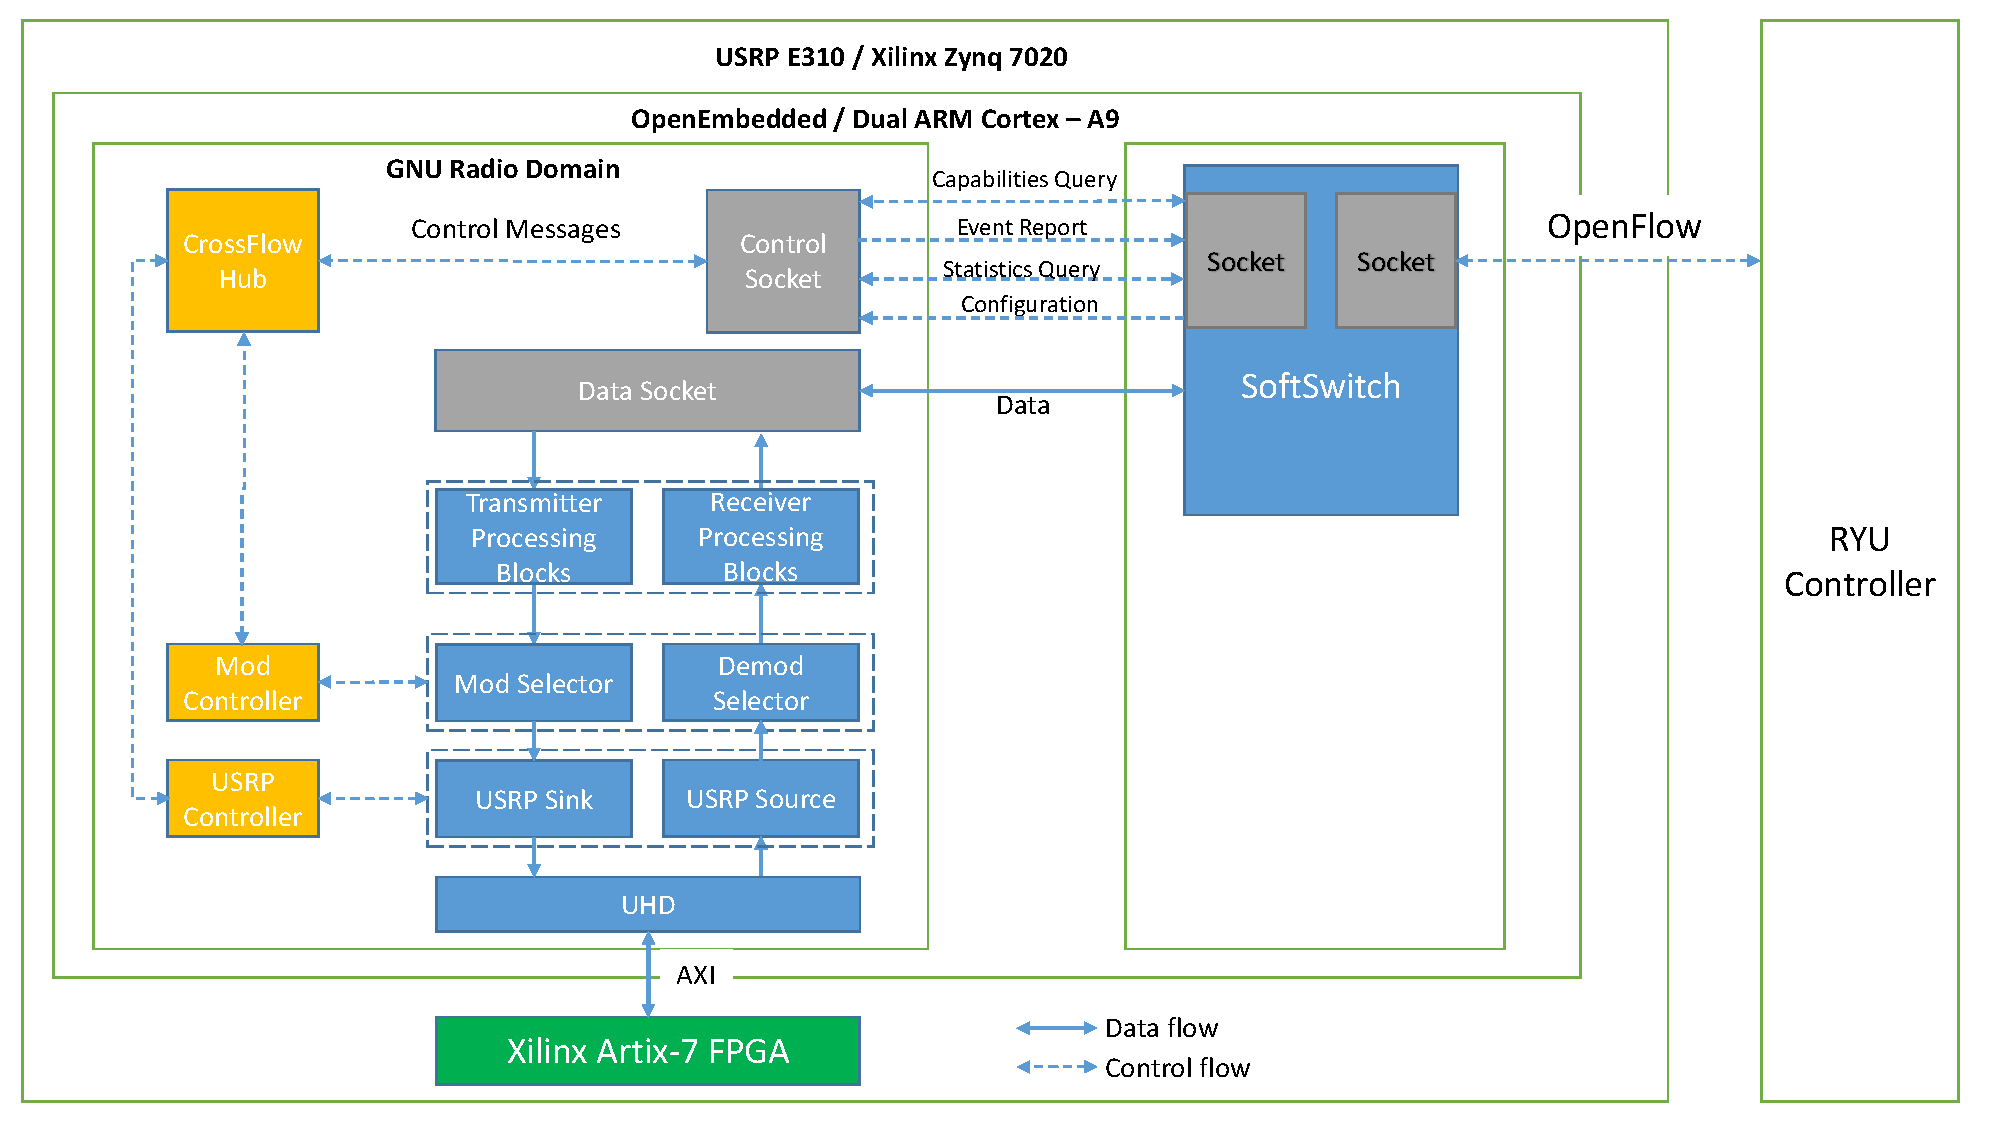
\includegraphics[width=0.8\textwidth]{figures/new.pdf}
%  \caption{Implementation of \crossflow}
%  \label{fig:message_block}
%\end{figure*}

\subsection{Data Plane abstractions}
\label{sec:data_plane}
We extend the data model proposed in \cite{Casey:14} to create an abstraction model for the \crossflow framework, which is displayed in Figure~\ref{fig:uml}. We build upon the \emph{radio physical port} concept proposed in \cite{aetherflow} to create a new layer of abstractions. This layer of abstractions exhibits a composition or \emph{has-a} relationship with the \emph{radio physical port} abstraction. This means that the blocks of this layer are the objects or members that comprise the \emph{radio physical port}. These blocks are derived from the most commonly used processing blocks in GNU Radio~\cite{gnuradio}. This abstract model serves the following design vision:

\begin{itemize}
\item From an application point of view, it allows visibility into the signal processing blocks, without going into implementation details.
\item It allows composition of blocks to implement new functionality, as this decision is handled by the higher \emph{radio physical port} abstraction. The application simply specifies the blocks to be connected for a specific wireless port instance and the internal framework handles the implementation.
\item It allows optional blocks to be put into the framework, which provides great flexibility for radio implementation. If any abstraction is not implemented, then we can use seamless emulation, switch offload or error indication techniques mentioned in \cite{Casey:14}.
\end{itemize}

In our current design, we focus on the first point of changing and quering the parameters of blocks at runtime. We assume that the number of blocks is fixed and the blocks can be connected in a consistent manner. From an application point of view, the application creates instances of the requisite blocks. In order to change parameters, the application needs to send \emph{<command,value>} tuple in a message. For query and receive event responses, it registers for events for each block and during an event, appropriate callbacks are invoked.    
One of the main requirements of the \crossflow model is that each abstraction should implement four types of interfaces as proposed in both \cite{Casey:14} and \cite{aetherflow}, namely: capabilities, configuration, statistics and events. The interface model for \crossflow provides the interfaces for a wireless radio port abstraction with only two processing blocks, \emph{Sink} and \emph{Modulators}. The Sink abstraction allows the controller to manage the signal sinks which can be a USRP device, file or a socket, while the Modulators abstraction allows management of modulation schemes (e.g., BPSK, QPSK, and 8PSK).

The interfaces for \emph{Sink} and \emph{Modulators} are categorized as follows:

%\textbf{Capabilities.}
\textbf{Sink.}
\begin{itemize}
\item \textbf{Capabilities}: The interface allows the controller to query the capabilities of sinks such as:
    (i)  Type of sink (USRP, socket, etc.);
    (ii) Channels supported;
    (iii) Center Frequency; and
    (iv) IP address.
\item \textbf{Configuration}: The interface allows the controller to configure properties of signal sinks such as:
    (i) Gain;
    (ii) Frequency, and
    (iii) Sample rate.
\item \textbf{Statistics}: The interface allows the controller to gather statistics for sinks such as:
    (i) Received Signal Strength Indicator (RSSI) and
    (ii) Temperature on-board.
\item \textbf{Events}: The interface allows the controller to take decisions based upon events in a sink such as:
    (i) Low or high RSSI and
    (ii) Low or high on-board temperature.
\end{itemize}

\textbf{Modulators.}
\begin{itemize}
\item \textbf{Capabilities}: The interface allows the controller to query the properties of the modulator block such as:
    (i) Modulations supported;
    (ii) Current samples/symbol; and
    (iii) Gray code.
\item \textbf{Configuration}: The interface allows the controller to configure properties of the modulator block such as:
    (i) Choice of modulation scheme (e.g. BPSK,QPSK and 8PSK);
    (ii) Sample/symbol; and
    (ii) Use of a Gray code.
\item \textbf{Statistics}: The interface allows the controller to gather statistics for the modulator block such as:
    (i) Signal to Noise Ratio (SNR) and
    (ii) Bit Error Rate(BER).
\item \textbf{Events}: The interface allows the controller to take decisions based upon events in the modulator block such as:
    (i) Low or high SNR and
    (ii) Low or high BER.
\end{itemize}

\subsection{Message Extensions}
\label{sec:messages}
  		  
\crossflow uses SDN design principles to control a network of configurable SDRs. As such, to enable control plane interactions between the SDN controller and the SDR, we had two options: either we could have implemented our own control protocol to enable their interactions or extend the existing OpenFlow \cite{openflow} framework. This is because OpenFlow does not natively support wireless features. In order to enable a cleaner implementation, we decided to extend OpenFlow by using experimenter messages within the OpenFlow protocol, similar to \aetherflow. This provides two advantages:
\begin{itemize}
\item We do not need to implement a new protocol for control and data plane interactions.
\item As we are using experimenter messages to carry \crossflow messages, the controller does not need to perform special handling for these messages. This enables the controller to remain independent of the underlying devices and hence it can handle both wired and wireless devices. 
\end{itemize} 

\chapter{\uppercase {Conclusion and Future Work}}
\label{sec:conclusion}

In this paper we presented two SDN frameworks \aetherflow and \crossflow.  These frameworks aim to bring the wireless networks into the SDN fold using a principled approach and provide greater flexibility and programmability in wireless networks. They provide new abstractions and extensions to demonstate a protocol independent architecture and provide proof-of-concept implementations to showcase flexible network management.

\aetherflow includes the ability to handle wireless packets using an OpenFlow
data path, remotely configure access points, query mobile
station capabilities and statistics, and report mobile station events.

To validate our ideas, we implemented an \aetherflow switch and adapted an
existing OpenFlow controller to work with our extensions of the OpenFlow
protocol. We experimented with an SDN-based mobile handoff application, and
found that our design slightly outperforms an optimized non-SDN application.
% We strongly
% suspect however, that we could improve throughput and packet loss with a more
% robust and reliable network configuration. In other words, for this specific
% wireless SDN application, there is much room to improve. However, 
We note this is a proof-of-concept experiment designed to show that useful SDN
applications can be written against the \aetherflow extensions to OpenFlow.

As a general  wireless SDN framework, the \aetherflow model can also
be immediately leveraged to support a number of different applications, or can
easily be extended to support them. In addition, similar extension approaches
can be used on systems other than IEEE~802.11, such as WiMAX or cellular
networks, which is a promising direction for the evolution of SDN. We leave this
as our future work.

% claim that support for other applications can be readily built using these SDN
% extensions.
% For example:
% 
% \begin{itemize}
% \item \emph{Client steering} could use centralized controller to track network
% probes for each client and filter the response set from those APs to a subset
% with strongest signal strength and least usage.
% 
% \item \emph{Mobile station and user-based QoS control} could combine
% client authentication with packet flow analysis to limit or accelerate
% traffic on the wireless network.
% 
% \item \emph{P2P content caching in APs} A centralized control could manage
% local AP caches by pushing blocks of frequently requested data or web pages
% directly to the APs where they are frequently used. This would require the
% entire network to understand application layer protocols.
% \end{itemize}
% 



On the other hand, the \crossflow framework allows flexible and real-time configuration of software defined radio interfaces from a network controller application. It allows a controller application to be written without worrying about the internal details of implementations. In order to validate our approach, we implemented \emph{frequency hopping} and \emph{adaptive modulation} applications. This shows that our design is viable and can extended to introduce new capabilities.

One of the challenges that we need to consider is the issue of latency between controller and SDR framework. The issue can be mitigated, by the introduction of distributed control module in SDR. The distributed control module will allow devices to take local decisions while the centralized controller is responsible for introducing policies and global management, thereby ensuring reduced latency.

The \crossflow framework can also be extended to allow controller to create GNU radio blocks and manipulate inter-connections between GNU radio blocks. It requires to design new API on switch agent and can be implemented by combining the methodology provided by GNU Radio. In GNU radio, each block has an input and output port and the application needs to specify the connecting ports in order to connect the blocks. Only ports which are similar, i.e, ports which operate on same types of data(message or stream), can connect to each other. The data type supported by a block can be obtained by sending capability messages. The decision whether two ports are compatible can be left to the application. 

Our results indicate that while current SDN protocols support the
development of very intelligent wireline network management applications, \aetherflow and \crossflow are
significant steps in bringing that same level of programmability to wireless
networks.

%\chapter{\uppercase {Architecture and Design}}
\label{sec:architecture}

In this section, we motivate and describe the overall architecture and design of \crossflow. In Section~\ref{sec:data_plane}, we introduce the proposed data plane abstractions. Then, in Section~\ref{sec:messages}, we describe how we extend the OpenFlow protocol to accommodate \crossflow messages.

%\begin{figure}[t]
%  \centering
%  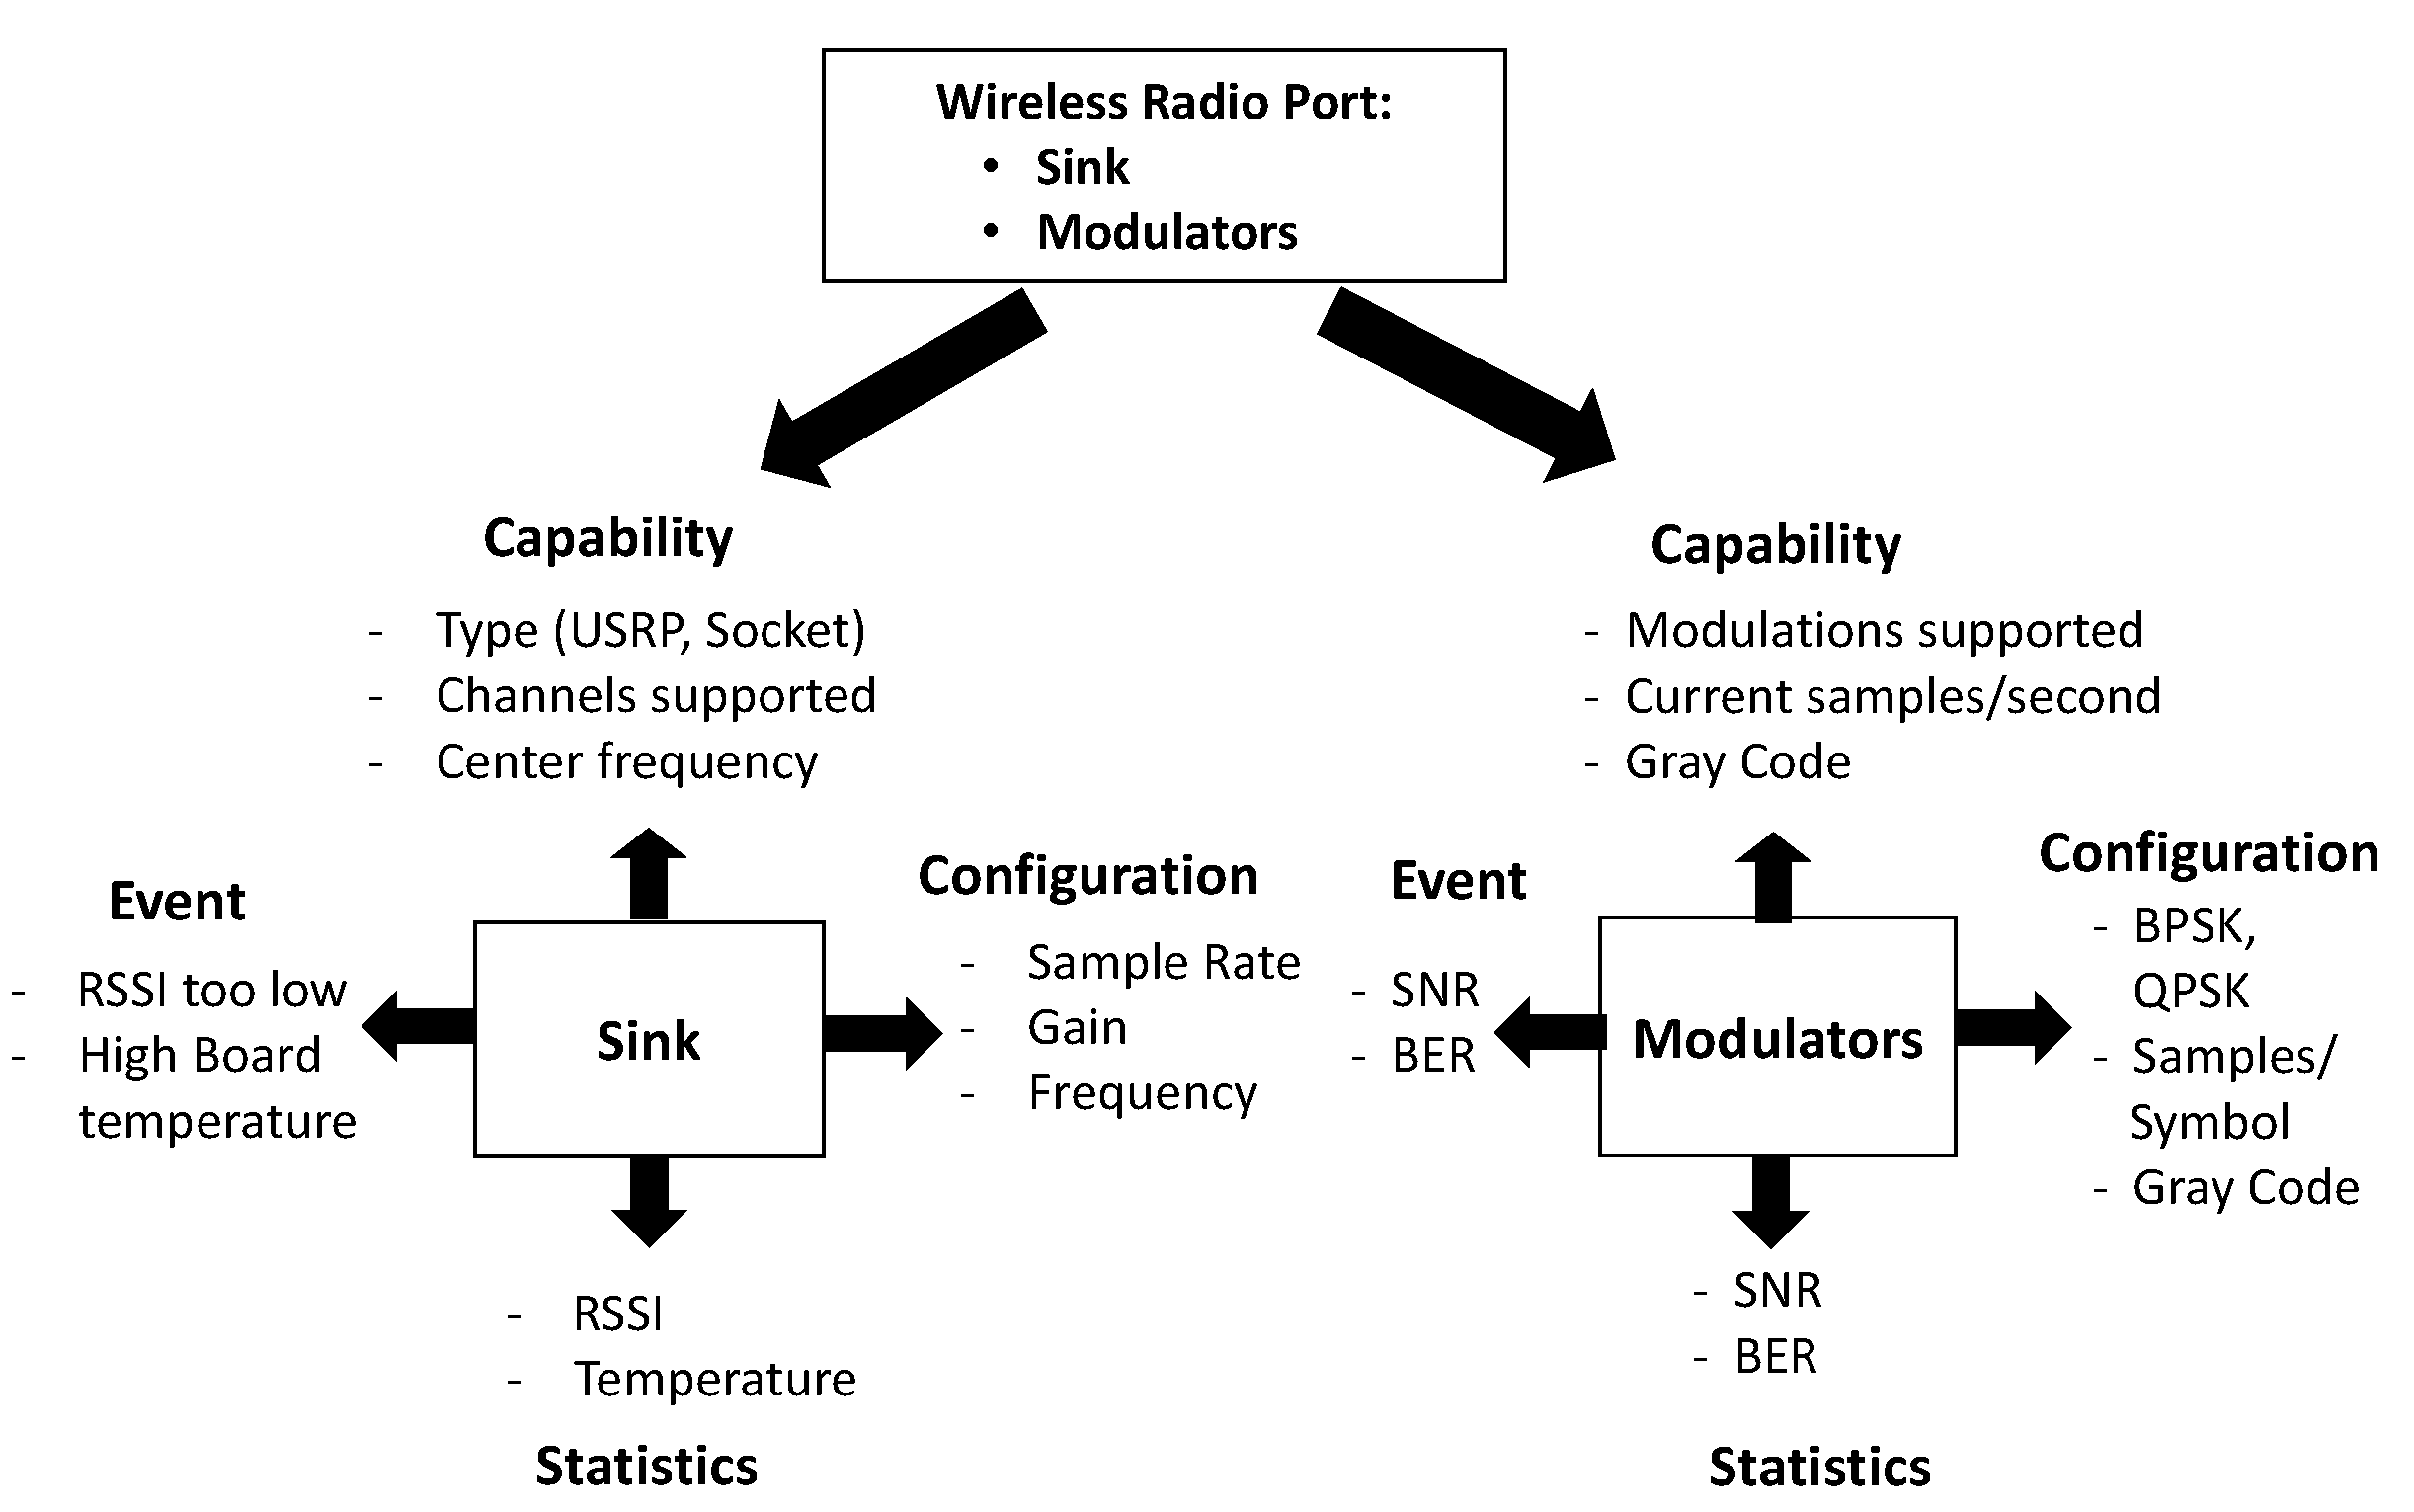
\includegraphics[width=0.48\textwidth]{figures/Interfaces.pdf}
%  \caption{Interface model for wireless radio port abstraction with two processing blocks: Sink and Modulators}
%  \label{fig:interface}
%\end{figure}

\begin{figure}[t]
  \centering
  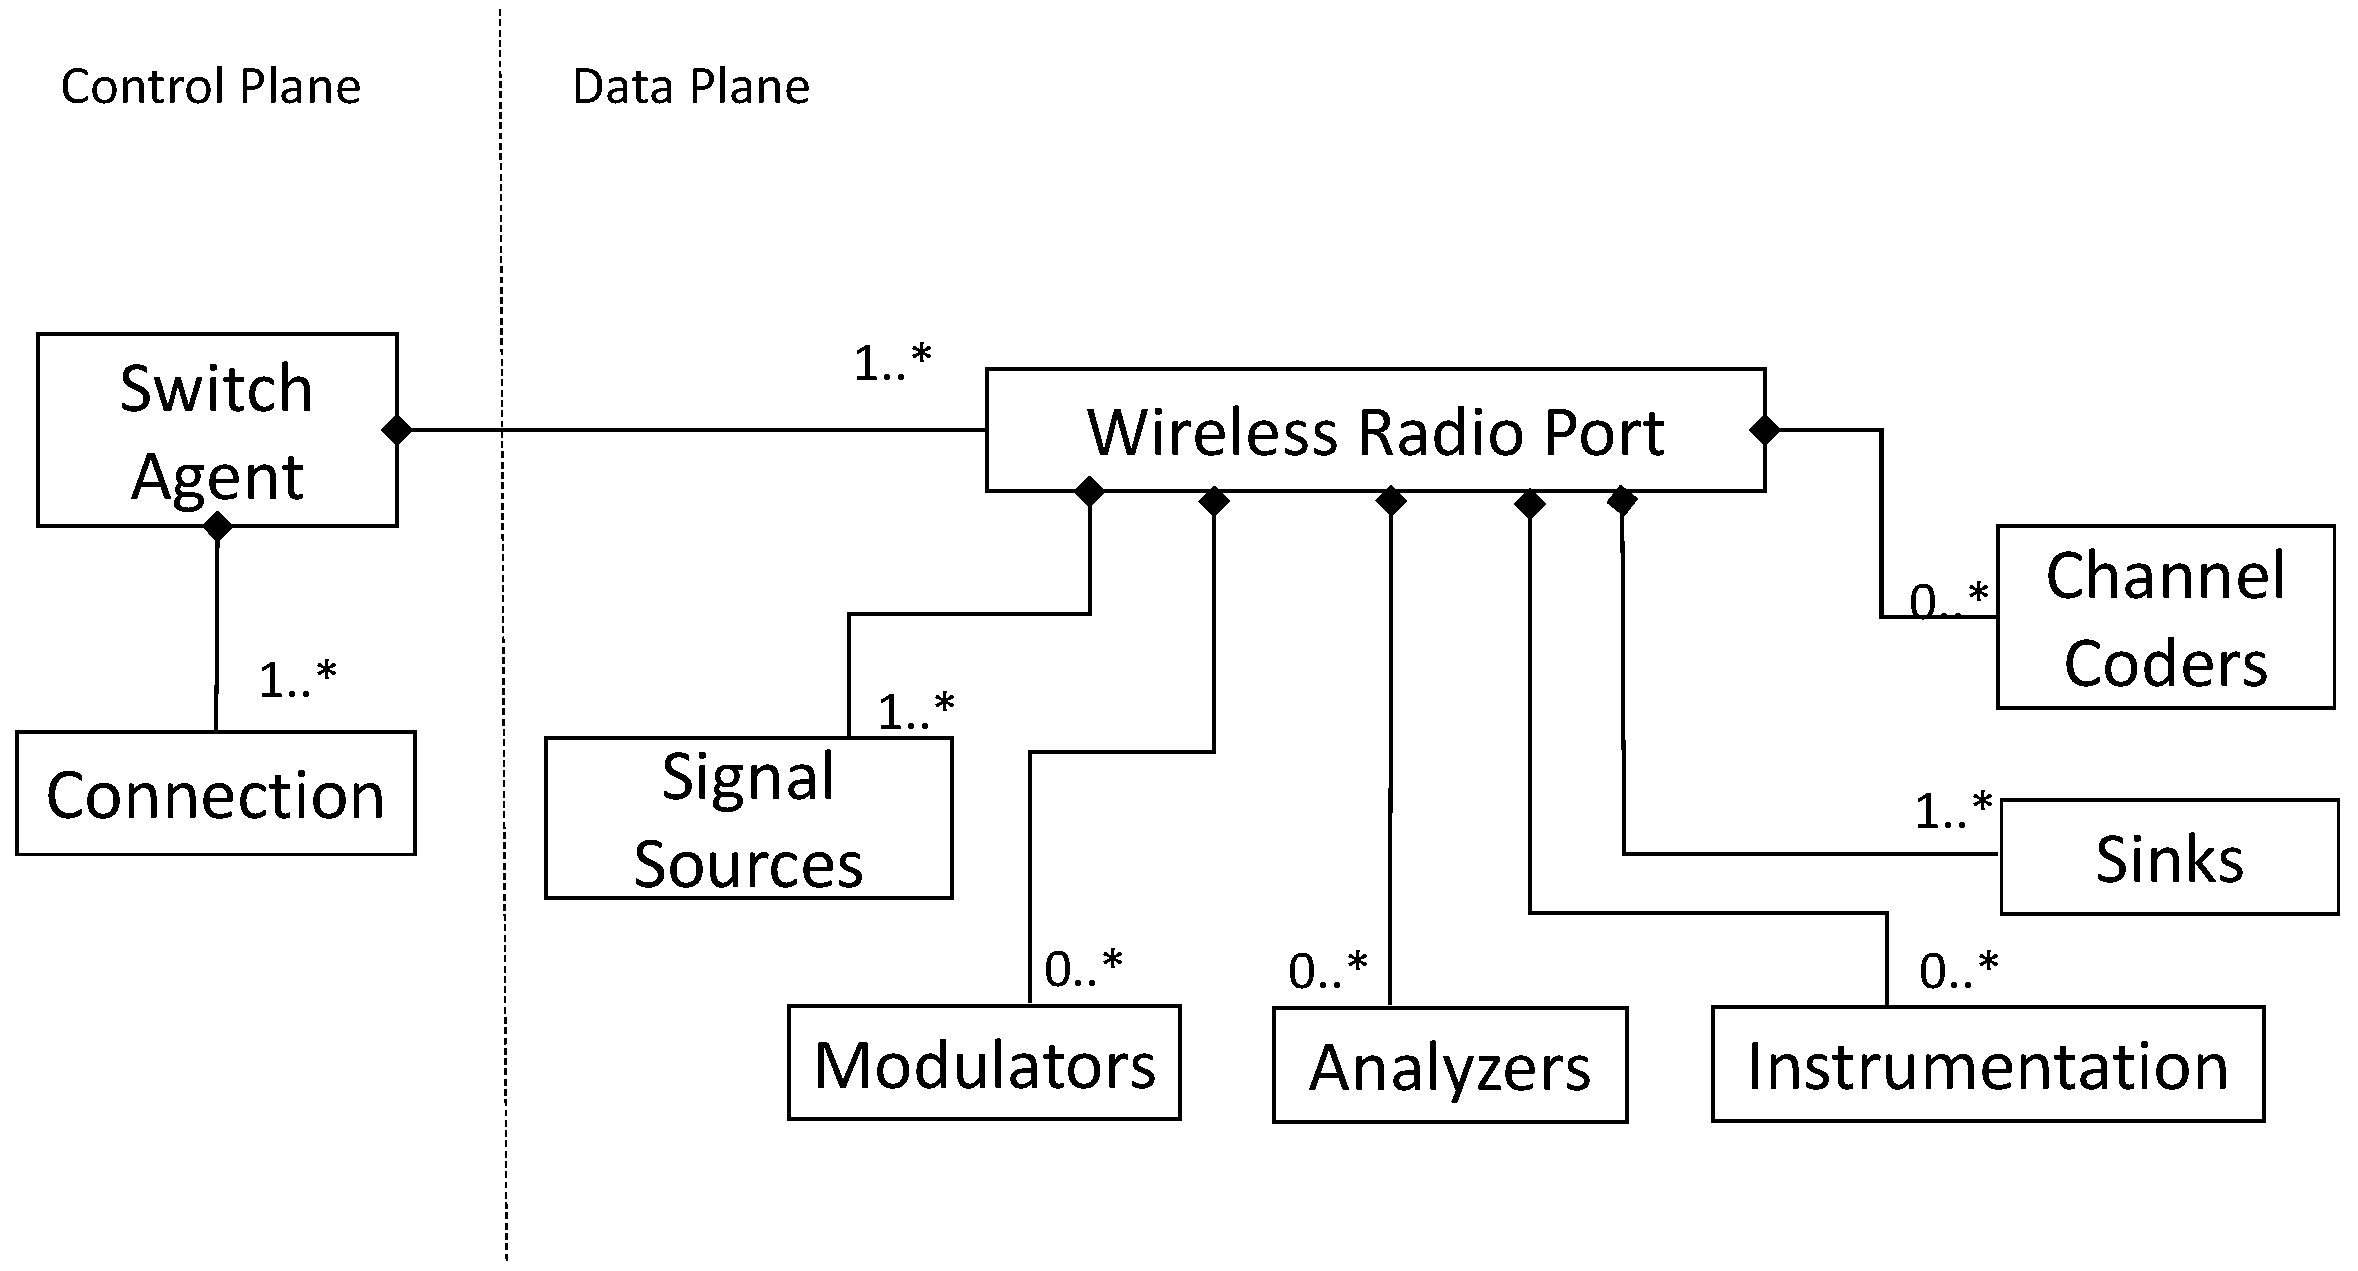
\includegraphics[width=1\textwidth]{figures/UML.pdf}
  \caption{Abstraction model of \crossflow}
  \label{fig:uml}
\end{figure}

%\begin{figure*}
%  \centering
%  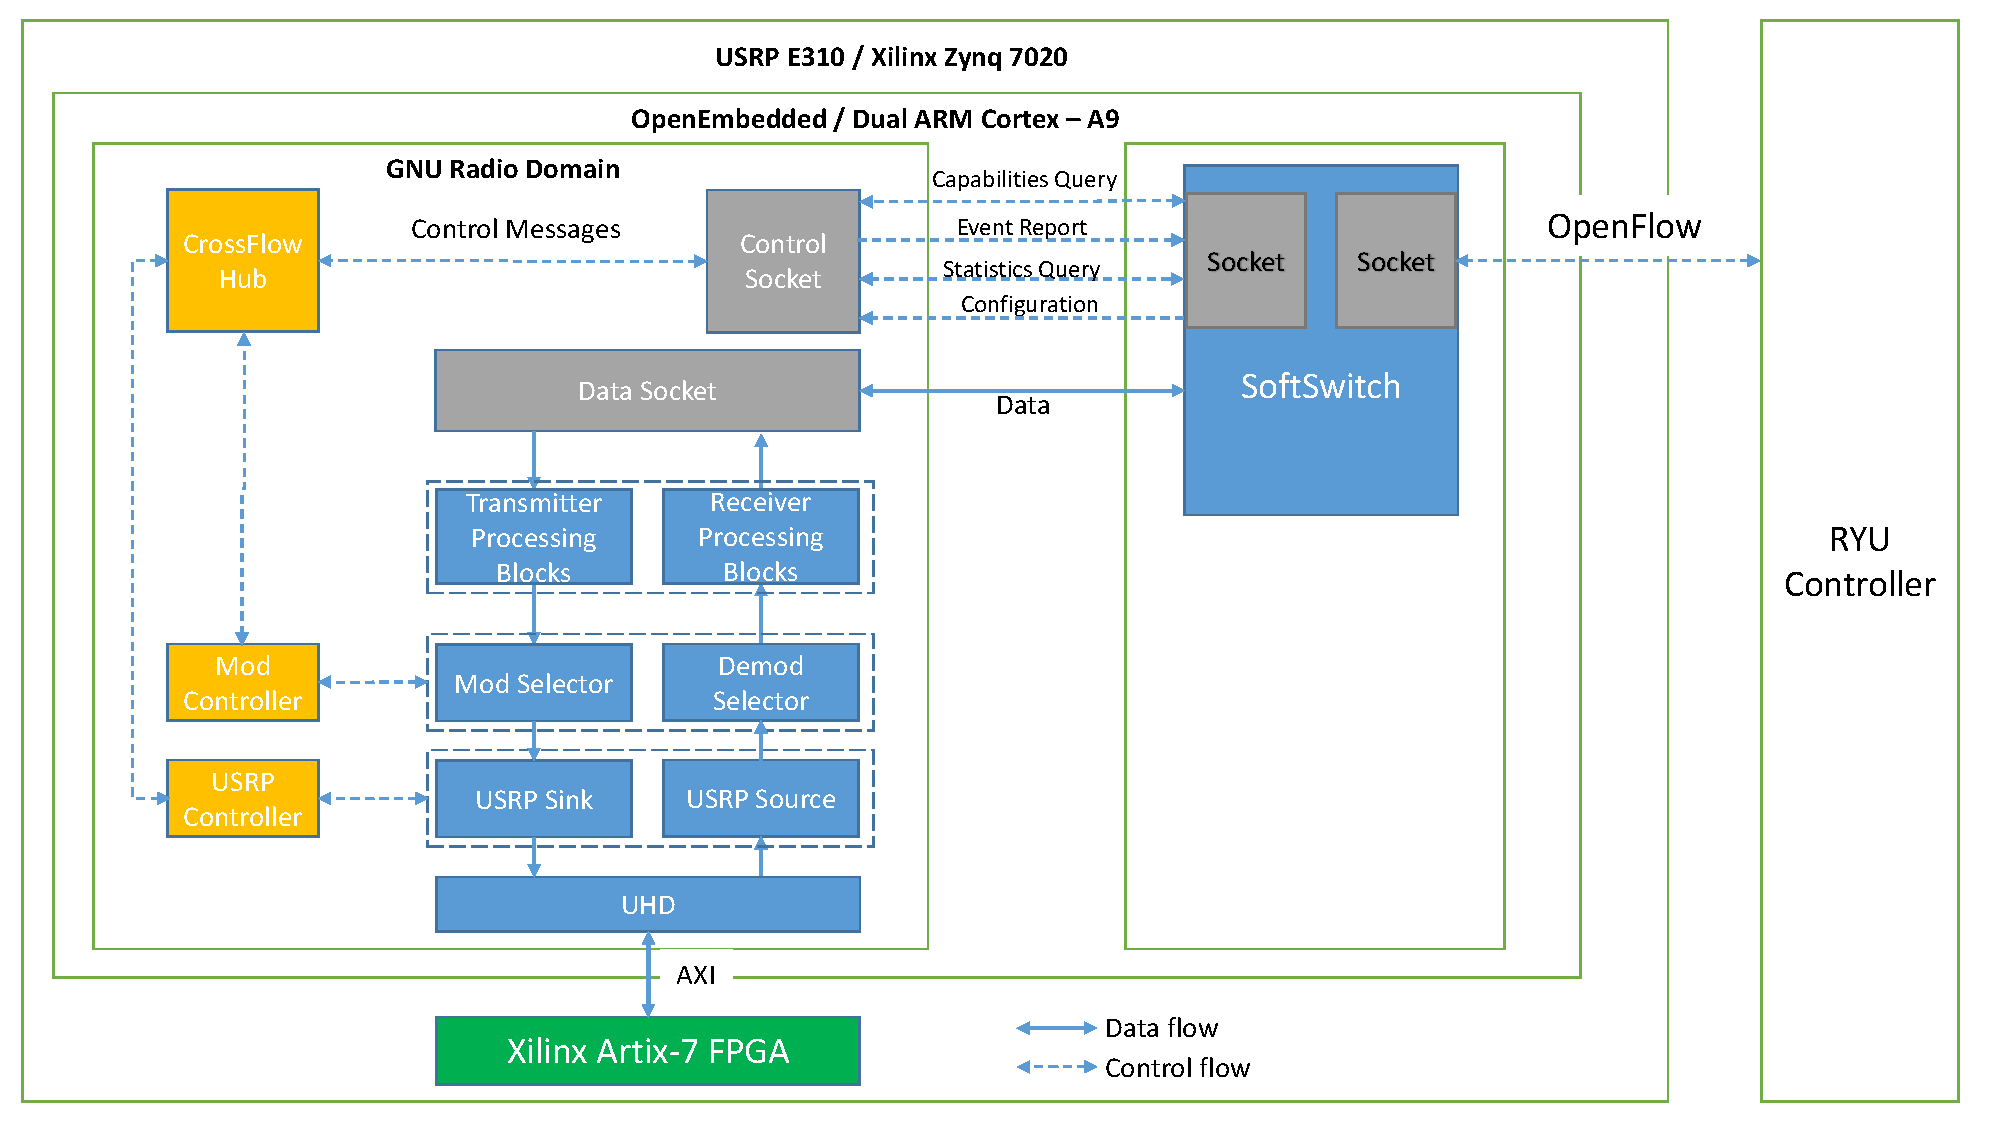
\includegraphics[width=0.8\textwidth]{figures/new.pdf}
%  \caption{Implementation of \crossflow}
%  \label{fig:message_block}
%\end{figure*}

\subsection{Data Plane abstractions}
\label{sec:data_plane}
We extend the data model proposed in \cite{Casey:14} to create an abstraction model for the \crossflow framework, which is displayed in Figure~\ref{fig:uml}. We build upon the \emph{radio physical port} concept proposed in \cite{aetherflow} to create a new layer of abstractions. This layer of abstractions exhibits a composition or \emph{has-a} relationship with the \emph{radio physical port} abstraction. This means that the blocks of this layer are the objects or members that comprise the \emph{radio physical port}. These blocks are derived from the most commonly used processing blocks in GNU Radio~\cite{gnuradio}. This abstract model serves the following design vision:

\begin{itemize}
\item From an application point of view, it allows visibility into the signal processing blocks, without going into implementation details.
\item It allows composition of blocks to implement new functionality, as this decision is handled by the higher \emph{radio physical port} abstraction. The application simply specifies the blocks to be connected for a specific wireless port instance and the internal framework handles the implementation.
\item It allows optional blocks to be put into the framework, which provides great flexibility for radio implementation. If any abstraction is not implemented, then we can use seamless emulation, switch offload or error indication techniques mentioned in \cite{Casey:14}.
\end{itemize}

In our current design, we focus on the first point of changing and quering the parameters of blocks at runtime. We assume that the number of blocks is fixed and the blocks can be connected in a consistent manner. From an application point of view, the application creates instances of the requisite blocks. In order to change parameters, the application needs to send \emph{<command,value>} tuple in a message. For query and receive event responses, it registers for events for each block and during an event, appropriate callbacks are invoked.    
One of the main requirements of the \crossflow model is that each abstraction should implement four types of interfaces as proposed in both \cite{Casey:14} and \cite{aetherflow}, namely: capabilities, configuration, statistics and events. The interface model for \crossflow provides the interfaces for a wireless radio port abstraction with only two processing blocks, \emph{Sink} and \emph{Modulators}. The Sink abstraction allows the controller to manage the signal sinks which can be a USRP device, file or a socket, while the Modulators abstraction allows management of modulation schemes (e.g., BPSK, QPSK, and 8PSK).

The interfaces for \emph{Sink} and \emph{Modulators} are categorized as follows:

%\textbf{Capabilities.}
\textbf{Sink.}
\begin{itemize}
\item \textbf{Capabilities}: The interface allows the controller to query the capabilities of sinks such as:
    (i)  Type of sink (USRP, socket, etc.);
    (ii) Channels supported;
    (iii) Center Frequency; and
    (iv) IP address.
\item \textbf{Configuration}: The interface allows the controller to configure properties of signal sinks such as:
    (i) Gain;
    (ii) Frequency, and
    (iii) Sample rate.
\item \textbf{Statistics}: The interface allows the controller to gather statistics for sinks such as:
    (i) Received Signal Strength Indicator (RSSI) and
    (ii) Temperature on-board.
\item \textbf{Events}: The interface allows the controller to take decisions based upon events in a sink such as:
    (i) Low or high RSSI and
    (ii) Low or high on-board temperature.
\end{itemize}

\textbf{Modulators.}
\begin{itemize}
\item \textbf{Capabilities}: The interface allows the controller to query the properties of the modulator block such as:
    (i) Modulations supported;
    (ii) Current samples/symbol; and
    (iii) Gray code.
\item \textbf{Configuration}: The interface allows the controller to configure properties of the modulator block such as:
    (i) Choice of modulation scheme (e.g. BPSK,QPSK and 8PSK);
    (ii) Sample/symbol; and
    (ii) Use of a Gray code.
\item \textbf{Statistics}: The interface allows the controller to gather statistics for the modulator block such as:
    (i) Signal to Noise Ratio (SNR) and
    (ii) Bit Error Rate(BER).
\item \textbf{Events}: The interface allows the controller to take decisions based upon events in the modulator block such as:
    (i) Low or high SNR and
    (ii) Low or high BER.
\end{itemize}

\subsection{Message Extensions}
\label{sec:messages}
  		  
\crossflow uses SDN design principles to control a network of configurable SDRs. As such, to enable control plane interactions between the SDN controller and the SDR, we had two options: either we could have implemented our own control protocol to enable their interactions or extend the existing OpenFlow \cite{openflow} framework. This is because OpenFlow does not natively support wireless features. In order to enable a cleaner implementation, we decided to extend OpenFlow by using experimenter messages within the OpenFlow protocol, similar to \aetherflow. This provides two advantages:
\begin{itemize}
\item We do not need to implement a new protocol for control and data plane interactions.
\item As we are using experimenter messages to carry \crossflow messages, the controller does not need to perform special handling for these messages. This enables the controller to remain independent of the underlying devices and hence it can handle both wired and wireless devices. 
\end{itemize} 

%%%%%%%%%%%%%%%%%%%%%%%%%%%%%%%%%%%%%%%%%%%%%%%%%%%%
%
%  New template code for TAMU Theses and Dissertations starting Fall 2012.  
%  For more info about this template or the 
%  TAMU LaTeX User's Group, see http://www.howdy.me/.
%
%  Author: Wendy Lynn Turner 
%	 Version 1.0 
%  Last updated 8/5/2012
%
%%%%%%%%%%%%%%%%%%%%%%%%%%%%%%%%%%%%%%%%%%%%%%%%%%%

%%%%%%%%%%%%%%%%%%%%%%%%%%%%%%%%%%%%%%%%%%%%%%%%%%%%%%%%%%%%%%%%%%%%%%
%%                           NOMENCLATURE
%%%%%%%%%%%%%%%%%%%%%%%%%%%%%%%%%%%%%%%%%%%%%%%%%%%%%%%%%%%%%%%%%%%%%

\chapter*{NOMENCLATURE}
\addcontentsline{toc}{chapter}{NOMENCLATURE}  % Needs to be set to part, so the TOC doesnt add 'CHAPTER ' prefix in the TOC.

\begin{tabular}{ll}
SDN & Software Defined Networking\tabularnewline
SDR & Software Defined Radio\tabularnewline
TLS & Transport Layer Security Protocol\tabularnewline
TCP & Transmission Control Protocol\tabularnewline
\end{tabular}

\vspace{2em}


\pagebreak{}


%%%%%%%%%%%%%%%%%%%%%%%%%%%%%%%%%%%%%%%%%%%%%%%%%%%%
%
%  New template code for TAMU Theses and Dissertations starting Fall 2012.  
%  For more info about this template or the 
%  TAMU LaTeX User's Group, see http://www.howdy.me/.
%
%  Author: Wendy Lynn Turner 
%	 Version 1.7
%  Last updated 3/24/2014
%
%%%%%%%%%%%%%%%%%%%%%%%%%%%%%%%%%%%%%%%%%%%%%%%%%%%
%%%%%%%%%%%%%%%%%%%%%%%%%%%%%%%%%%%%%%%%%%%%%%%%%%%%%%%%%%%%%%%%%%%%%%
%%       TABLE OF CONTENTS
%%%%%%%%%%%%%%%%%%%%%%%%%%%%%%%%%%%%%%%%%%%%%%%%%%%%%%%%%%%%%%%%%%%%%
% single-space sections in Table of Contents  - commented in version 1.7
%\renewcommand{\cftsecafterpnum}{\vskip0.5\baselineskip}
%\renewcommand{\cftsubsecafterpnum}{\vskip0.5\baselineskip}
%\renewcommand{\cftsubsubsecafterpnum}{\vskip0.5\baselineskip}
%%%%%%%%%%%%%%%%%%%%%%%%%%%%%%%%%%%%%%%%%%%%%%%%%%%

\phantomsection
\addcontentsline{toc}{chapter}{TABLE OF CONTENTS}  

\begin{singlespace}
\renewcommand\contentsname{\normalfont} {\centerline{TABLE OF CONTENTS}}

%\setcounter{tocdepth}{4} % This puts \subsubsection[]{×} in your List of Tables.  The default is 3.


%%%%%%%%%%%%%  Adds Page above the page number in TOC
\setlength{\cftaftertoctitleskip}{1em}
\renewcommand{\cftaftertoctitle}{%
\hfill{\normalfont {Page}\par}}



\tableofcontents

\end{singlespace}

\pagebreak{}

%%%%%%%%%%%%%%%%%%%%%%%%%%%%%%%%%%%%%%%%%%%%%%%%%%%%%%%%%%%%%%%%%%%%%%
%%                           LIST OF FIGURES
%%%%%%%%%%%%%%%%%%%%%%%%%%%%%%%%%%%%%%%%%%%%%%%%%%%%%%%%%%%%%%%%%%%%%

\phantomsection
\addcontentsline{toc}{chapter}{LIST OF FIGURES}  

\renewcommand{\cftloftitlefont}{\center\normalfont\MakeUppercase}

\setlength{\cftbeforeloftitleskip}{-12pt} %% Positions the LOF title vertically to match the chapter titles
\renewcommand{\cftafterloftitleskip}{12pt}


\renewcommand{\cftafterloftitle}{%
\\[4em]\mbox{}\hspace{2pt}FIGURE\hfill{\normalfont Page}\vskip\baselineskip}

\begingroup


\begin{center}
\begin{singlespace}
%% These values make the lof table entries appear double spaced between.
\setlength{\cftbeforechapskip}{0.4cm}
\setlength{\cftbeforesecskip}{0.30cm}
\setlength{\cftbeforesubsecskip}{0.30cm}
\setlength{\cftbeforefigskip}{0.4cm}
\setlength{\cftbeforetabskip}{0.4cm} 

\listoffigures

\end{singlespace}
\end{center}

\pagebreak{}


%%%%%%%%%%%%%%%%%%%%%%%%%%%%%%%%%%%%%%%%%%%%%%%%%%%%%%%%%%%%%%%%%%%%%%
%%                           lIST OF TABLES
%%%%%%%%%%%%%%%%%%%%%%%%%%%%%%%%%%%%%%%%%%%%%%%%%%%%%%%%%%%%%%%%%%%%%%
%%
%\phantomsection
%\addcontentsline{toc}{chapter}{LIST OF TABLES}  

%\renewcommand{\cftlottitlefont}{\center\normalfont\MakeUppercase}

%\setlength{\cftbeforelottitleskip}{-12pt} %% Positions the LOT title vertically to match the chapter titles

%\renewcommand{\cftafterlottitleskip}{12pt}


%\renewcommand{\cftafterlottitle}{%
%\\[4em]\mbox{}\hspace{4pt}TABLE\hfill{\normalfont Page}\vskip\baselineskip}

%\begin{center}
%\begin{singlespace}

%% These values make the lot table entries appear double spaced between.
%\setlength{\cftbeforechapskip}{0.4cm}
%\setlength{\cftbeforesecskip}{0.30cm}
%\setlength{\cftbeforesubsecskip}{0.30cm}
%\setlength{\cftbeforefigskip}{0.4cm}
%\setlength{\cftbeforetabskip}{0.4cm}

%\listoftables 

%\end{singlespace}
%\end{center}
%\endgroup
%\pagebreak{}  % Need this for the pagenumbering to be correct. 
  % This is simply a file that formats and adds your toc, lof, and lot, please do not edit this unless you have a specific need. .

%\include{section1}
%\include{section2}
%\include{section3}

%fix spacing in bibliography, if any...
%%%%%%%%%%%%%%%%%%%%%%%%%%%%%%%%%%%%%%%%%%%%%%%%%%%%%%%%%%%%%
\let\oldbibitem\bibitem
\renewcommand{\bibitem}{\setlength{\itemsep}{0pt}\oldbibitem}
%%%%%%%%%%%%%%%%%%%%%%%%%%%%%%%%%%%%%%%%%%%%%%%%%%%%%%%%%%%%%%%
%%%%%%%%%%%%%%%%%%%%%%%%%%%%%%%%%%%%%%%%%%%%%%%%%%%
%
%  New template code for TAMU Theses and Dissertations starting Fall 2012.  
%  For more info about this template or the 
%  TAMU LaTeX User's Group, see http://www.howdy.me/.
%
%  Author: Wendy Lynn Turner 
%	 Version 1.0 
%  Last updated 8/5/2012
%
%%%%%%%%%%%%%%%%%%%%%%%%%%%%%%%%%%%%%%%%%%%%%%%%%%%


%%%%%%%%%%%%%%%%%%%%%%%%%%%%%%%%%%%%%%%%%%%%%%%%%%%%%%%%%%%%%%%%%%%%%%
%%                           REFERENCES 
%%%%%%%%%%%%%%%%%%%%%%%%%%%%%%%%%%%%%%%%%%%%%%%%%%%%%%%%%%%%%%%%%%%%%

\phantomsection
\addcontentsline{toc}{chapter}{REFERENCES}

\renewcommand{\bibname}{{\normalsize\rm REFERENCES}}

\bibliographystyle{plain}
\bibliography{references}
% %%%%%%%%%%%%%%%%%%%%%%%%%%%%%%%%%%%%%%%%%%%%%%%%%%%
%
%  New template code for TAMU Theses and Dissertations starting Fall 2012.  
%  For more info about this template or the 
%  TAMU LaTeX User's Group, see http://www.howdy.me/.
%
%  Author: Wendy Lynn Turner 
%	 Version 1.0 
%  Last updated 8/5/2012
%
%%%%%%%%%%%%%%%%%%%%%%%%%%%%%%%%%%%%%%%%%%%%%%%%%%%

\begin{appendices}
\titleformat{\chapter}{\centering\normalsize}{APPENDIX \thechapter}{0em}{\vskip .5\baselineskip\centering}
\renewcommand{\appendixname}{APPENDIX}

%%%%%%%%%%%%%%%%%%%%%%%%%%%%%%%%%%%%%%%%%%%%%%%%%%%
%
%  New template code for TAMU Theses and Dissertations starting Fall 2012.  
%  For more info about this template or the 
%  TAMU LaTeX User's Group, see http://www.howdy.me/.
%
%  Author: Wendy Lynn Turner 
%	 Version 1.0 
%  Last updated 8/5/2012
%
%%%%%%%%%%%%%%%%%%%%%%%%%%%%%%%%%%%%%%%%%%%%%%%%%%%

%%%%%%%%%%%%%%%%%%%%%%%%%%%%%%%%%%%%%%%%%%%%%%%%%%%%%%%%%%%%%%%%%%%%%%
%%                           APPENDIX A 
%%%%%%%%%%%%%%%%%%%%%%%%%%%%%%%%%%%%%%%%%%%%%%%%%%%%%%%%%%%%%%%%%%%%%

\phantomsection

\chapter{\uppercase{First Appendix}}

Text for the Appendix follows.

\begin{figure}[H]
\centering
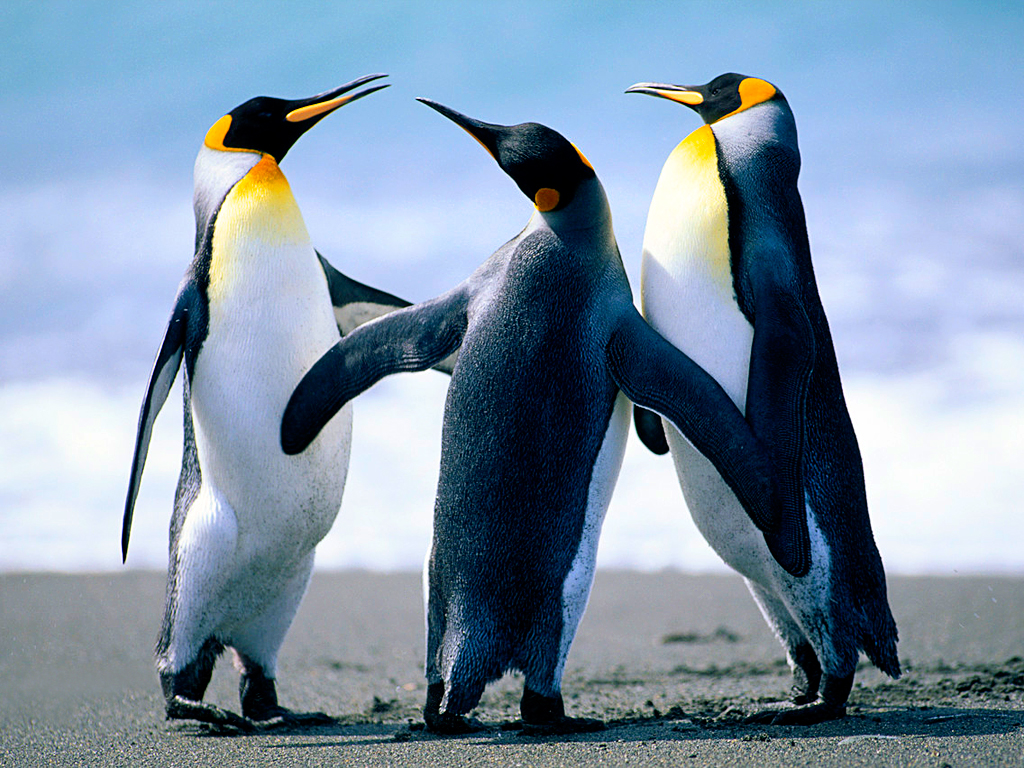
\includegraphics[scale=.50]{figures/Penguins.jpg}
\caption{TAMU figure}
\label{fig:tamu-fig5}
\end{figure}

%%%%%%%%%%%%%%%%%%%%%%%%%%%%%%%%%%%%%%%%%%%%%%%%%%%
%
%  New template code for TAMU Theses and Dissertations starting Fall 2012.  
%  For more info about this template or the 
%  TAMU LaTeX User's Group, see http://www.howdy.me/.
%
%  Author: Wendy Lynn Turner 
%	 Version 1.0 
%  Last updated 8/5/2012
%
%%%%%%%%%%%%%%%%%%%%%%%%%%%%%%%%%%%%%%%%%%%%%%%%%%%

%%%%%%%%%%%%%%%%%%%%%%%%%%%%%%%%%%%%%%%%%%%%%%%%%%%%%%%%%%%%%%%%%%%%%%
%%                           APPENDIX B
%%%%%%%%%%%%%%%%%%%%%%%%%%%%%%%%%%%%%%%%%%%%%%%%%%%%%%%%%%%%%%%%%%%%%

\chapter{\uppercase {Second Appendix with a longer title - much longer in fact}}

Text for the Appendix follows.

\begin{figure}[H]
\centering
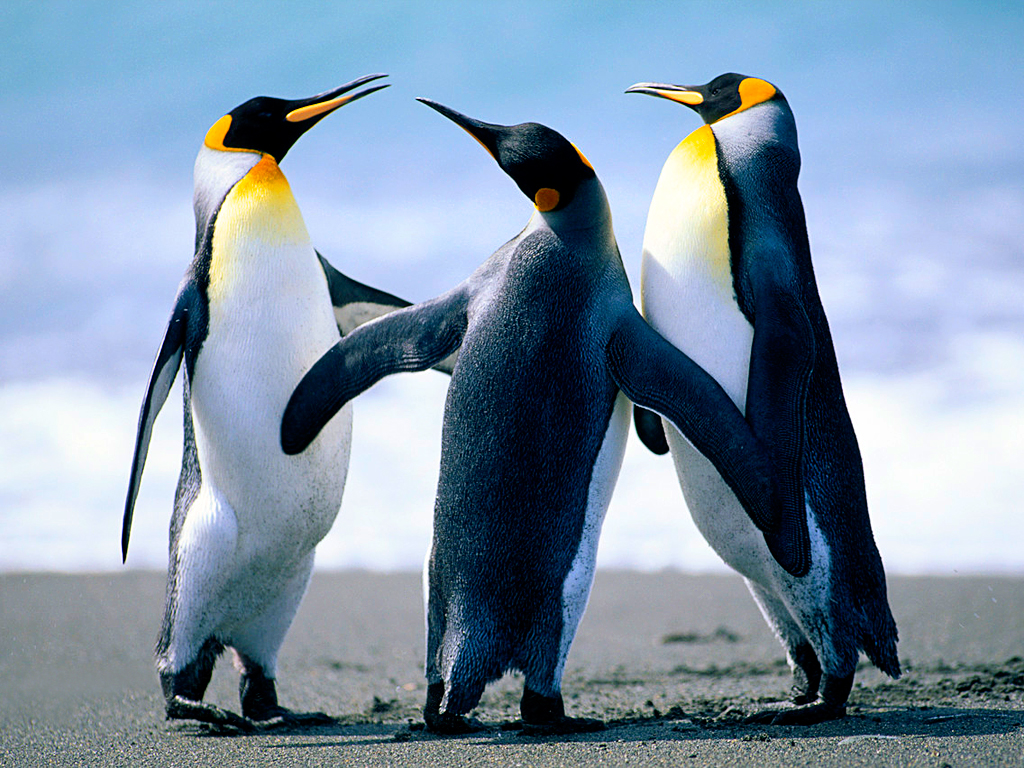
\includegraphics[scale=.50]{figures/Penguins.jpg}
\caption{TAMU figure}
\label{fig:tamu-fig6}
\end{figure}

\section{Appendix Section}


\pagebreak{}

\end{appendices}


\end{document}
